% Chapter Template

\chapter{Datos} % Main chapter title

\label{Cap_Data} % Change X to a consecutive number; for referencing this chapter elsewhere, use \ref{ChapterX}


%Justificación de la importancia de graficar los datos antes de realizar análisis estadísticos.
Previo a la realización de los análisis esadísticos correspondientes para responder a la interrogante planteada respecto de la existencia de los patrones identificados en Memoria de Reconocimiento como Efecto Espejo en una tarea de detección perceptual, los datos obtenidos fueron explorados de manera exhaustiva graficando las posibles correlaciones entre la ejecución de los participantes y diversas variables operantes en el mismo. Graficar los datos antes de someterlos a un análisis constituye una práctica altamente recomendable, ya que 1) permite evaluar la pertinencia de los experimentos propuestos a la luz de las respuestas obtenidas por los participantes y 2) constituye un primer filtro para descartar la posibilidad de que los participantes estuvieren respondiendo de manera incongruente con las tareas presentadas, procurando tener una mayor confianza en las conclusiones que puedan extraerse de su análisis.\\

%Presentación de los controles graficados: Atención, El efecto del paso del tiempo y las variables externas en los estímulos. 
En este capítulo se presentan gráficas que exploran la posible relación que pudieran tener las respuestas de los participantes con cualquier variable ajena a las demandas de la tarea, como podrían ser las respuestas inmediatamente anteriores (i.e. trenes de respuesta), el paso del tiempo (i.e. aprendizaje) y las propiedades de los estímulos diseñados (i.e. sesgo). Idealmente, se esperaría que el desempeño de los participantes no mostrara cambios a lo largo del tiempo y no variara en función a ninguna característica de los estímulos construidos que no sea el número de círculos externos en las figuras de Ebbinghaus, (i.e. la variable independiente).\\









\section{Control 1: ¿Los participantes estaban poniendo atención a la tarea para emitir una respuesta?}

%Evaluando la atención: Que
Los experimentos realizados estuvieron compuestos de 640 ensayos a lo largo de los cuales los participantes tuvieron que 1) decidir si los estímulos presentados cumplían con la condición que se les solicitó detectar y 2) valorar su certidumbre sobre esta primer respuesta asignándole un puntaje. Dada la extensión y lo demandante del procedimiento, la primer preocupación era que los participantes se agotaran y dejaran de poner atención a la tarea al emitir sus respuestas. Para controlar esta posibilidad, se revisaron las respuestas emitidas ensayo a ensayo para verificar que todas las opciones de respuesta fueran utilizadas para cada tarea planteada y que no se presentaran trenes de respuesta que pudieran sugerir una emisión de respuestas independiente del contenido de la tarea.\\

\begin{itemize}
\item Emisión de respuestas 'Sí/No' a lo largo del experimento.

Primero se graficaron las respuestas emitidas ensayo a ensayo durante la tarea de detección binaria ('Sí, los círculos son iguales', 'No, los círculos son diferentes'). El objetivo principal de estas gráficas fue el de detectar trenes de respuesta prolongados que, dada la aleatoriedad con que los estímulos fueron presentados por el programa, pudieran delatar un sesgo del participante a presionar una tecla en particular independientemente del estímulo a evaluar en pantalla.\\

%Participante representativo: Respuestas 'No' por 80 ensayos
La Figura~\ref{fig:Resp_E1_P1} ilustra la importancia de revisar los datos antes de incluirlos en el análisis estadístico y extraer conclusiones, al presentar las respuestas emitidas a la tarea de detección binaria por el Participante 1 del Experimento 2, quien pasó los primeros 80 ensayos del experimento respondiendo repetidamente a la tecla 'No'. Este tren de respuesta es lo suficientemente largo como para cuestionar la atención con que el Participante 1 estuvo respondiendo a la tarea.\\ 

\begin{figure}[th]
\centering
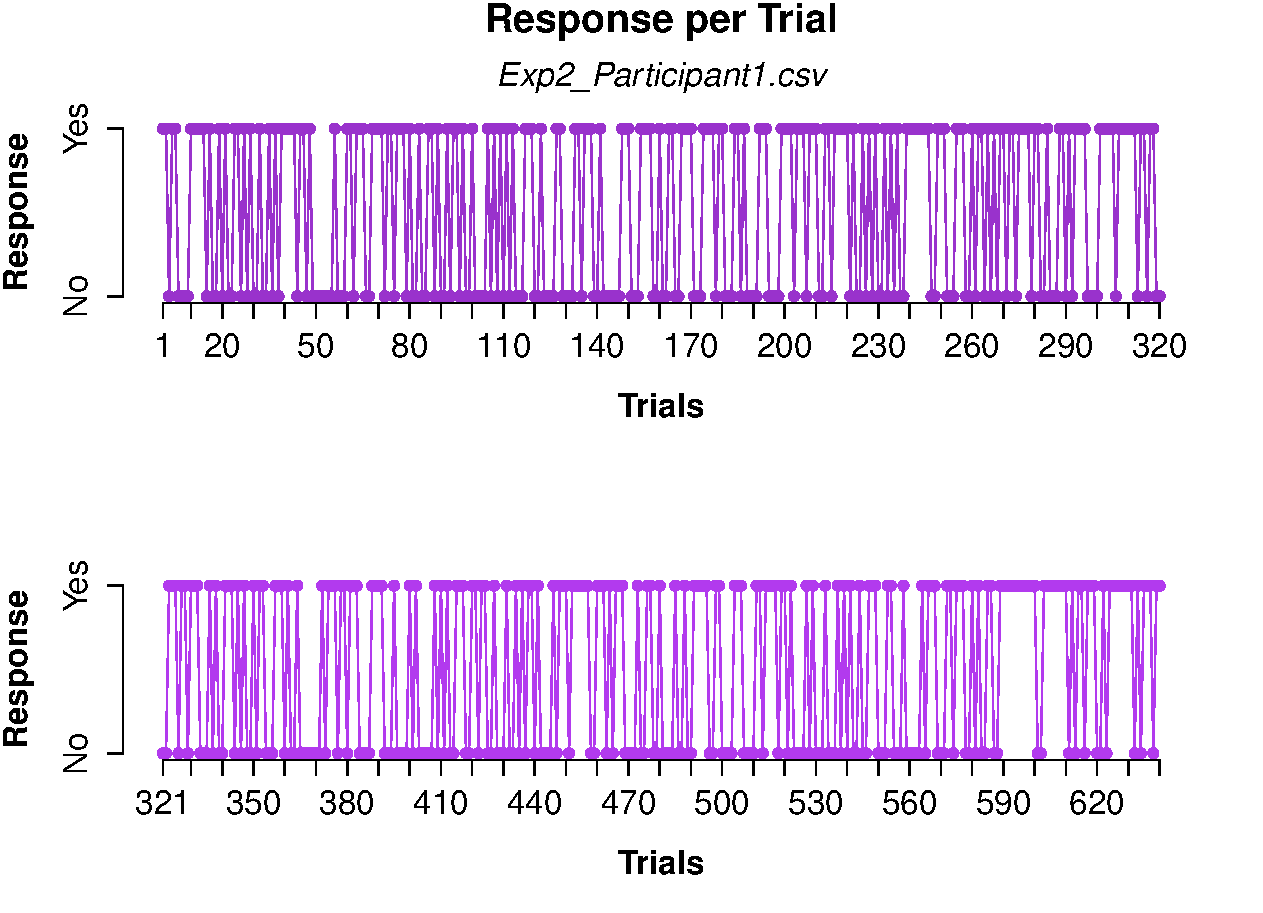
\includegraphics[width=0.60\textwidth]{Figures/Response_Exp2_P1} 
%\decoRule
\caption[Respuesta emitida por ensayo; ejemplo de participante sesgado]{Se muestran las respuestas ('Sí/No') emitidas en cada uno de los 640 ensayos del Experimento 1 por el Participante 1. La gráfica superior muestra los primeros 320 ensayos y la gráfica inferior, los 320 restantes. En el panel superior se aprecia con claridad un tren de respuesta que se extiende a lo largo de 80 ensayos, durante los cuales el Participante 1 sólo utilizó una de las opciones de respuesta.}
\label{fig:Resp_E1_P1}
\end{figure}

Las gráficas correspondientes al resto de los participantes en los Experimentos 1 y 2, se muestran en las Figuras~\ref{fig:Response_P1} y \ref{fig:Response_E2}, respectivamente.\\

\item Correlación entre las respuestas 'Sí/No' emitidas y el tipo de estímulo presentado en cada ensayo.

A continuación, se graficaron las respuestas emitidas por los participantes en cada ensayo añadiendo indicadores que señalaran las características de los estímulos presentados; en concreto, si se trataba de una señal o ruido y si se trataba de un estímulo fácil o difícil.\\ 

Retomando el caso del Participante 1 del Experimento 2 presentado en la Figura~\ref{fig:Resp_E1_P1}, la Figura~\ref{fig:BiasResp_E1_P1} explora la posible correlación entre las respuestas registradas y el tipo de estímulo presentado en cada ensayo. Sin embargo, parece ser que el tren de 80 respuestas 'No' consecutivas se mantiene con independencia del tipo de estímulo presentado. Con base en dicha evidencia, se decidió eliminar al Participante 1 del Experimento 2 del análisis estadístico, pues se cree que se tiene razones suficientes para dudar de la atención que el participante estaba prestando al responder a la tarea.\\

\begin{figure}[th]
\centering
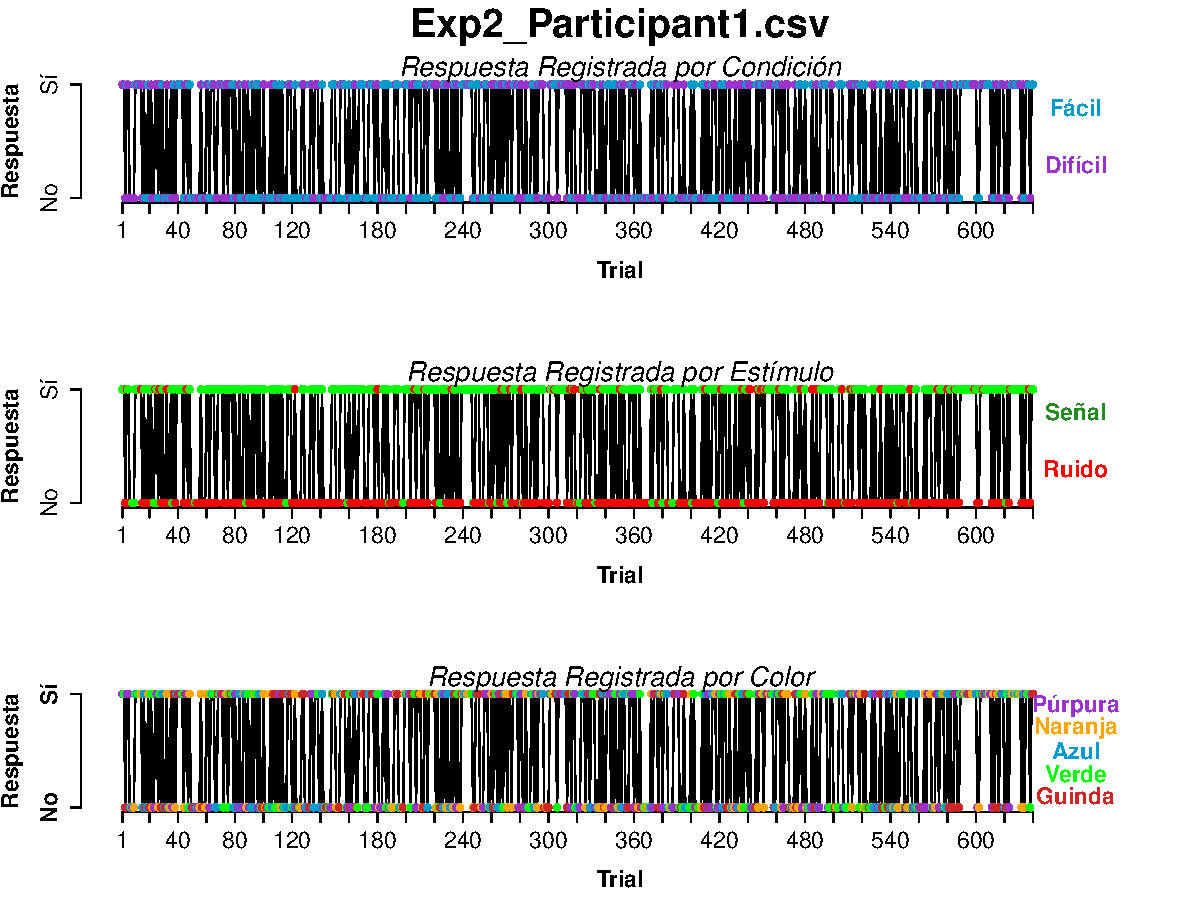
\includegraphics[width=0.60\textwidth]{Figures/BiasResp_Exp2_P1} 
%\decoRule
\caption[Respuesta por Tipo de Estimulo; ejemplo de participante sesgado]{Se muestran las respuestas registradas por el Participante 1 en cada uno de los ensayos del Experimento 2, indicando con diferentes colores el tipo de estímulo que se le mostraba en cada ocasión. En el panel superior se señala con colores violeta y azul si el estímulo presentado pertenecía a la categoría Difícil o Fácil, respectivamente. En el panel inferior se indica si se trataba de una señal o ruido, señalándolos con los colores verde y rojo, respectivamente.}
\label{fig:BiasResp_E1_P1}
\end{figure}

Las Figuras~\ref{fig:BiasResp_E1} y () muestran las gráficas correspondientes al resto de los participantes en el Experimento 1 y 2, respectivamente.\\

\item Asignación de puntajes de confianza, ('1','2' y '3').

En la segunda fase de la tarea, los participantes tenían tres opciones de respuesta (teclas '1', '2' y '3') para señalar qué tanta confianza tenían sobre la respuesta previa ('poco seguro', 'más o menos seguro' o 'muy seguro', respectivamente). Las respuestas emitidas eran registradas por el programa de acuerdo a una escala mayor, (con valores del 1 al 6), que diferencía entre la confianza de haber rechazado correctamente un estímulo con ruido (e.g. '1, estoy seguro de que los círculos eran diferentes') y la confianza de haber identificado correctamente un estímulo con la señal a detectar (e.g '6, estoy seguro de que los círculos son iguales'), dejando los valores intermedios de la escala (3 y 4) para los puntajes que correlacionaran con una confianza baja en la respuesta emitida (e.g. '3, poco seguro de que los círculos eran diferentes' y '4, poco seguro de que los círculos eran iguales').\\

Tal y como se hizo para la tarea de detección binaria, se graficaron los puntajes de confianza asignados por los participantes en cada uno de los 640 ensayos que conformaron los experimentos. La Figura~\ref{fig:Rating_E2_P4} muestra los puntajes emitidos por el Participante 15 del Experimento 2 a lo largo de la tarea. Este participante, de acuerdo con lo que se esperaría de alguien que estuviere prestando atención a la tarea, utiliza todas las opciones de respuesta (teclas '1', '2' y '3'), siendo estas registradas por el programa de acuerdo con la respuesta dada a la tarea de detección binaria ('1' como '3' o '4', '2' como '2' o '5', '3' como '1' o '6'; dependiendo si la respuesta previa fue un 'no' o un 'sí', respectivamente).\\ 
 
\begin{figure}[th]
\centering
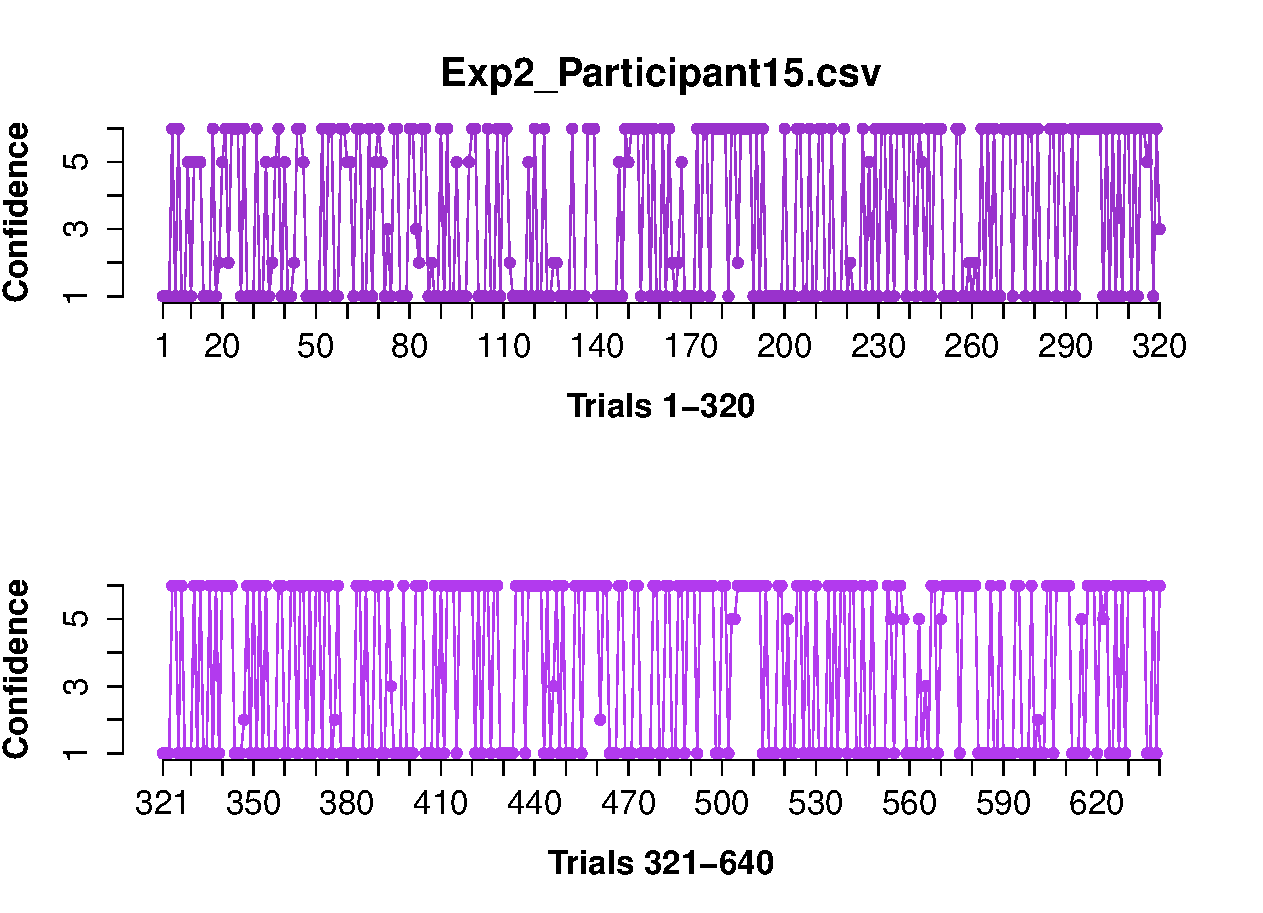
\includegraphics[width=0.60\textwidth]{Figures/Rating_Exp2_P15} 
%\decoRule
\caption[Asignacion Puntaje de confianza: Ejemplo]{Se muestran los puntajes de confianza asignados por el Participante 15 del Experimento 1 a las respuestas emitidas en la tarea binaria, durante cada uno de los 640 ensayos que conforman el experimento. El panel superior muestra los puntajes asignados en los primeros 320 ensayos del experimento; el panel inferior, muestra los 320 restantes.}
\label{fig:Rating_E2_P4}
\end{figure}

El registro ensayo a ensayo de los puntajes de confianza asignados por el resto de los participantes en los Experimentos 1 y 2 se muestran en las Figuras~\ref{fig:Rating_E1} y \ref{fig:Rating_E2}, respectivamente.\\

\end{itemize}








\section{Control 2: ¿La duración del experimento tuvo un impacto en la ejecución de los participantes?}

La fatiga y la habituación a la ilusión constituyen dos grandes preocupaciones que se tuvieron a la hora de diseñar los experimentos, mismas que se buscó prevenir añadiendo controles tales como la pantalla de espera entre ensayos (para dar a los participantes la oportunidad de estirarse o descansar, hasta que se sintieran listos para atender al siguiente estímulo) y la exposición limitada a los estímulos a comparar por 1.5 segundos (para preveer que la ilusión perdiera fuerza mientras más tiempo pasaran los participantes estudiando la figura). Teniendo esto en mente, se realizó un segundo conjunto de gráficas para verificar que efectivamente el desempeño de los participantes no mostraran indicios de un posible efecto de la fatiga  o de habituación a la tarea, decayendo o mejorando con el paso de los ensayos respectivamente.\\ 


\begin{itemize}
\item Aciertos y errores a lo largo del tiempo

Primero, se construyeron gráficas que permitieran observar emsayo a ensayo si los participantes habían respondido de manera correcta, o no. Este tipo de gráficas permiten evaluar de manera general si existen cambios en el desempeño de los participantes a lo largo del tiempo, conforme estos adquieren más experiencia con la tarea.\\

La Figura~\ref{fig:Success_E1_P14} muestra el desempeño del Participante 14 a lo largo del Experimento 2. En la gráfica superior se presenta el registro acumulativo de aciertos y errores a lo largo del experimento, mientras que en los paneles inferiores a esta se muestra, ensayo a ensayo, si la respuesta dada en cada ensayo fue identificada como acierto o error.\\


\begin{figure}[th]
\centering
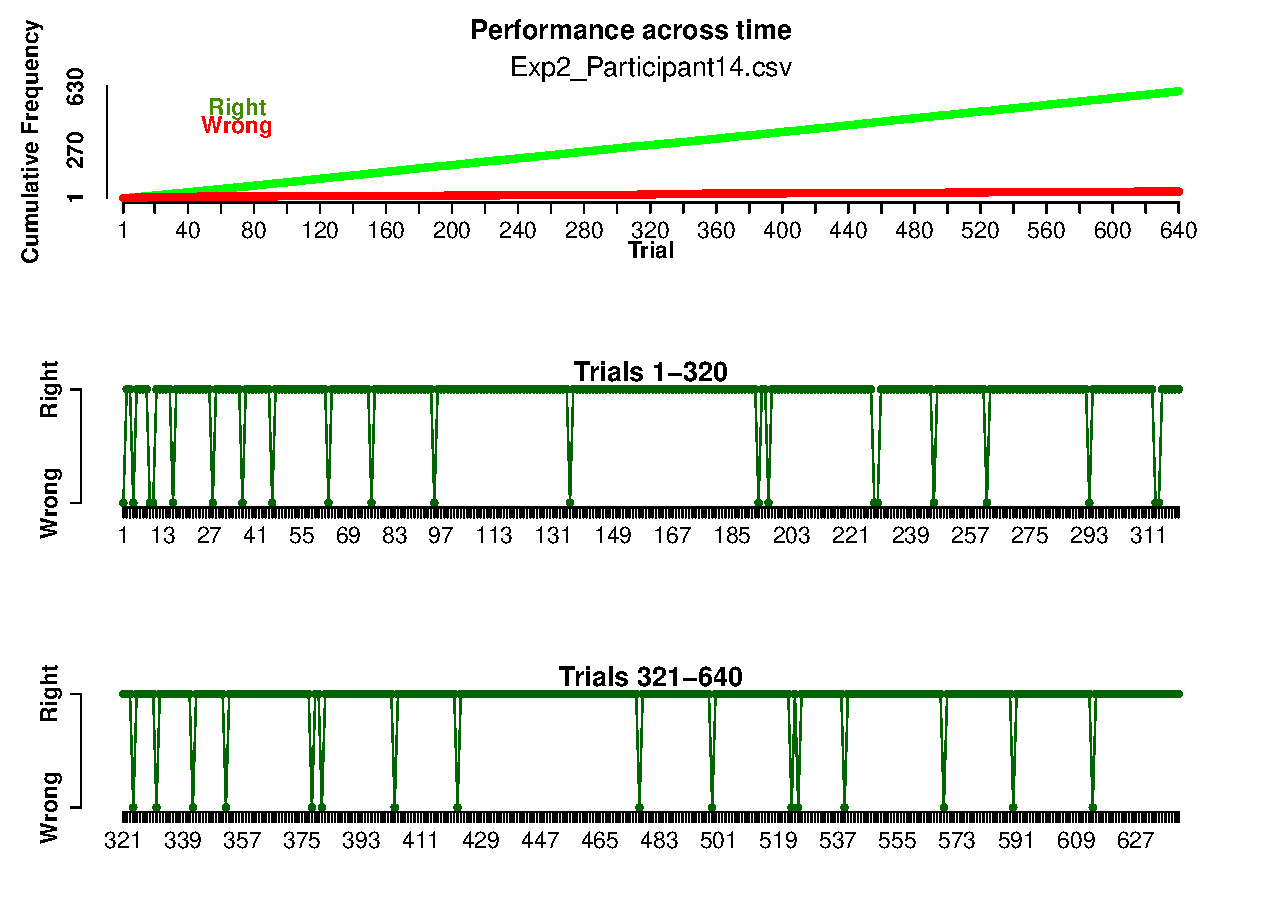
\includegraphics[width=0.60\textwidth]{Figures/Success_Exp2_P14}
%\decoRule
\caption[Aciertos y errores a lo largo del tiempo: Participante ejemplar]{Aciertos y errores cometidos por el Participante 14 del Experimento 1. En el panel superior se muestra el registro acumulativo de estos a lo largo del experimento, en tanto que los paneles inferiores muestran, ensayo a ensayo, la clasificación de las respuestas del participante como Acierto o Error, de acuerdo con el estímulo evaluado. Al respecto de estos últimos se señala que el panel medio muestra la primera mitad del experimento y el panel inferior, el resto.}
\label{fig:Success_E1_P14}
\end{figure}

Las Figuras~\ref{fig:Success_E1} y \ref{fig:Success_E2} muestran los aciertos y errores cometidos a lo largo de los experimentos por el resto de los participantes en los Experimentos 1 y 2, respectivamente.\\


\item Resultados a lo largo del tiempo

Además de identificar de las respuestas emitidas por los participantes a lo largo de los experimentos como aciertos o errores, se realizó un gráfico que distinguía entre los dos posibles tipos de aciertos y errores en una tarea de detección (hits o rechazos correctos y falsas alarmas u omisiones, respectivamente).\\ 

La Figura~\ref{fig:Outcome_E1_P14} muestra una vez más la ejecución del Participante 14 del Experimento 2, en términos de los resultados obtenidos (i.e. la etiqueta dada a sus respuestas en relación a si fueron, o no, acertadas) a lo largo de la tarea. El panel superior muestra el registro acumulativo de cada uno de los cuatro posibles resultados a lo largo del experimento, en tanto que el panel inferior muestra el resultado obtenido en cada uno de los ensayos.\\ 

\begin{figure}[th]
\centering
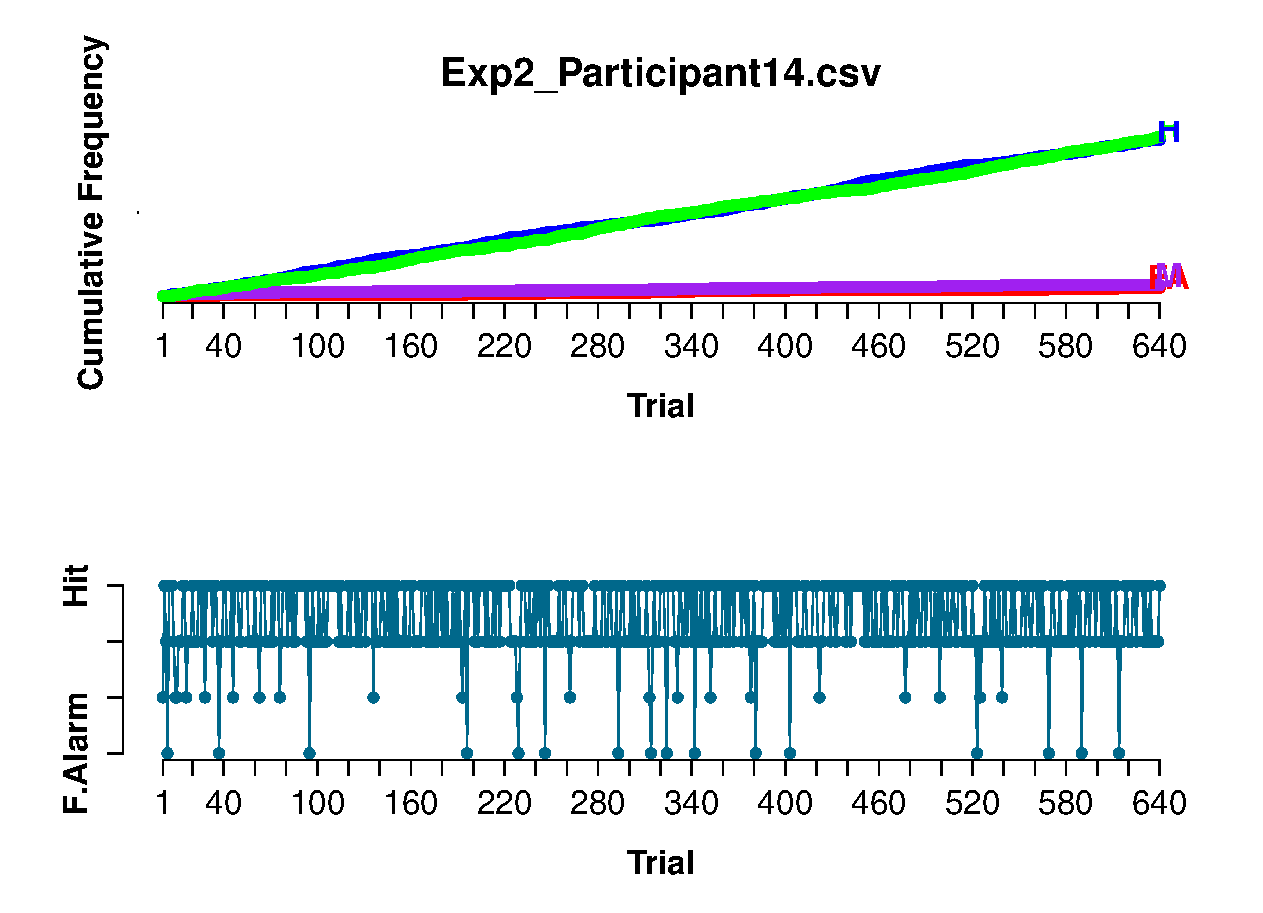
\includegraphics[width=0.60\textwidth]{Figures/Outcome_Exp2_P14}
%\decoRule
\caption[Resultado obtenido a lo largo del tiempo: Ejemplo]{Resultado obtenido por el Participante 6 del Experimento 2, dada cada una de sus respuestas a lo largo del Experimento. El panel superior muestra la frecuencia acumulada de Hits, Falsas Alarmas, Rechazos y Omisiones obtenidos durante el experimento; el panel inferior muestra el tipo de resultado registrado en cada uno de los 640 ensayos.}
\label{fig:Outcome_E1_P14}
\end{figure}

El resto de los participantes en los experimentos 1 y 2 aparecen en las Figuras~\ref{fig:Outcome_E1} y \ref{fig:Outcome_E2}, respectivamente.\\

\end{itemize}











\section{Control 3: ¿Las variables mezcladas para construir los estímulos están afectando el desempeño de los participantes?}

Como se recordará del Capítulo 3, donde se detalla la construcción de los estímulos utilizados en cada uno de los experimentos, la variable deliberadamente manipulada para construir las dos condiciones de dificultad entre las cuales se compara el desempeño de los participantes fue el número de círculos externos en las figuras de Ebbinghaus. Sin embargo, es importante descartar la posibilidad de que el desempeño de los participantes variara en relación a otro tipo de características de los estímulos presentados, como podrían ser los distintos colores en que fueron mostrados cada uno de los estímulos diseñado a lo largo de sus 8 o 10 presentaciones, dependiendo el experimento.\\

\begin{itemize}
\item El efecto del Color sobre la intensidad de la ilusión.

En términos del tipo de influencia que pueden tener las características de los estímulos construidos sobre la ejecución de los participantes, una primer posibilidad es que éstas pudieran estar teniendo un impacto en la intensidad de la ilusión perceptual utilizada. Por ejemplo, sería razonable tener dudas respecto de si los distintos colores en que aparecen cada uno de los estímulos diseñados podría estar alterando la manera en que los participantes responden a los mismos.\\ 

\begin{figure}[th]
\centering
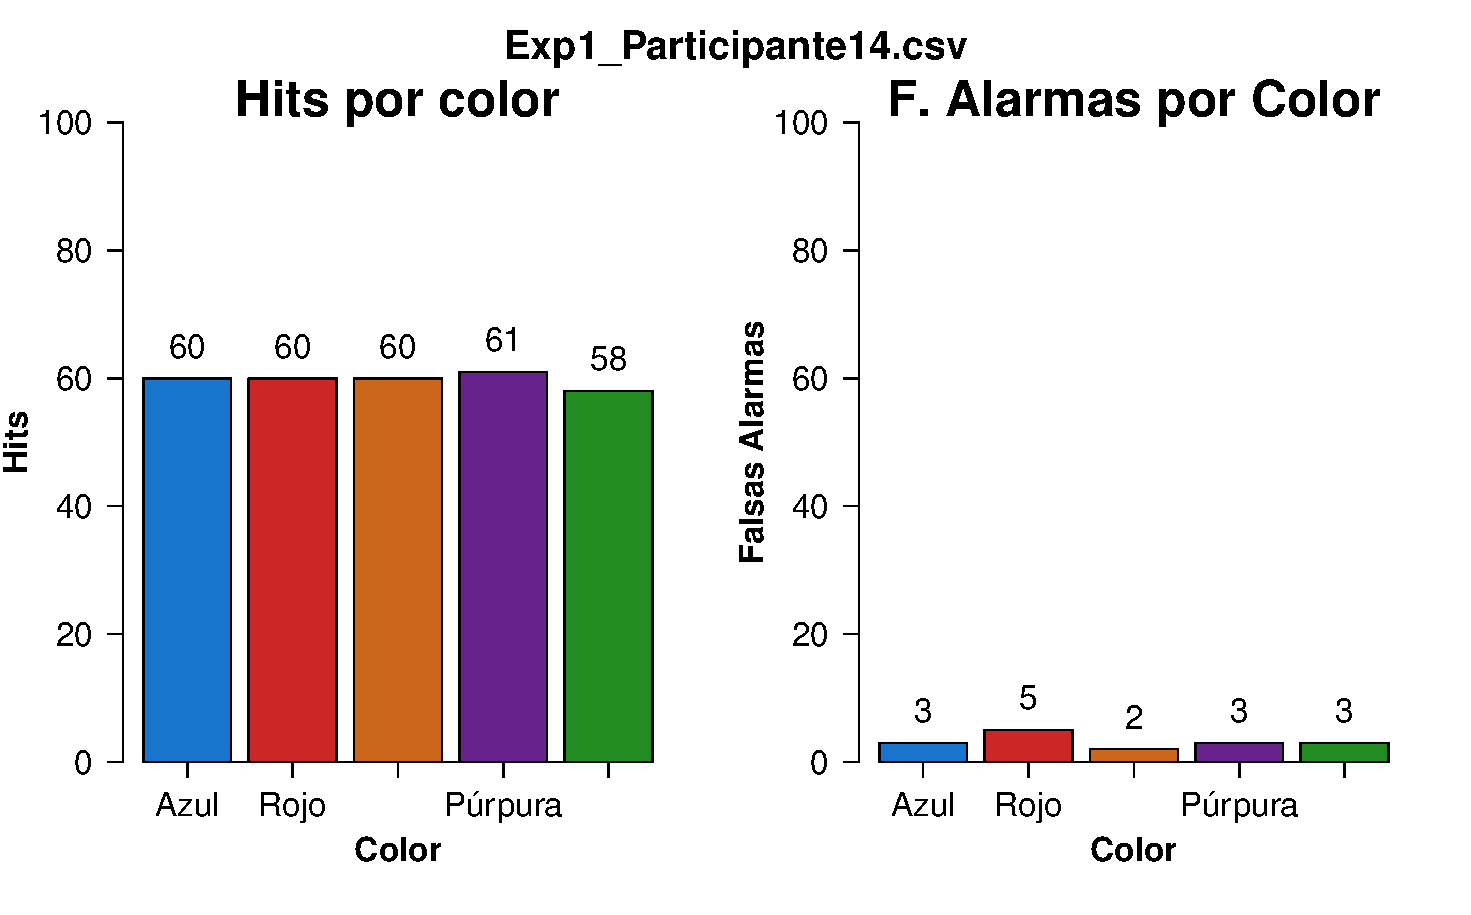
\includegraphics[width=0.60\textwidth]{Figures/Color_Exp1_P14}
%\decoRule
\caption[Hits y Falsas Alarmas por Color; Ejemplo]{Se muestra el desempeño del Participante 14 del Experimento 1 en relación al color de los estímulos. En el panel izquierdo se muestra la relación entre el número de Hits obtenidos y el color de los estímulos, mientras que en el panel derecho se muestra la misma relación para las Falsas alarmas.}
\label{fig:Color_E2_P14}
\end{figure}

La Figura~\ref{fig:Color_E2_P14} muestra la relación entre los Hits y las Falsas alarmas cometidas por el Participante 14 a lo largo del Experimento 2, en relación con el color de las figuras. De acuerdo con las gráficas desplegadas, no parece ser que el color de las figuras tenga un efecto sobre el desempeño de este participante. Se muestran únicamente los Hits y las Falsas Alarmas, pensando que arrojan información suficiente respecto de los aciertos y errores cometidos a lo largo del experimento, en tanto que mantienen una relación complementaria con el número de Omisiones y Rechazos correctos, proporcionando de manera implícita la frecuencia absoluta de estos últimos.\\

Las gráficas correspondientes a la relación entre las frecuencias absolutas de Hits y Falsas Alarmas y el color de los estímulos, para el resto de los participantes en los Experimentos 1 y 2 se encuentran en la Figura~\ref{fig:Color_E1} y \ref{fig:Color_E2}, respectivamente. 

\item El Efecto del Color sobre la respuesta de los participantes.

Una segunda forma en que el color de los estímulos podría estar alterando el desempeño de los participantes, sería si estos mostraran alguna preferencia a responder de cierta forma ante uno o más de los colores utilizados, con independencia del resto de las características presentes en los estímulos.\\

La Figura~\ref{fig:BiasCol_E1_P13} muestra la proporción de Respuestas 'Sí'/'No' emitidas por el Participante 13 del Experimento 1 para cada uno de los diferentes colores en que fueron presentados los estímulos. Como se puede ver en la figura, parece ser que en general la proporción se mantiene a lo largo de los distintos colores para este participante, por lo que no parece ser que el color esté influyendo en su manera de responder a los estímulos construidos.

\centering
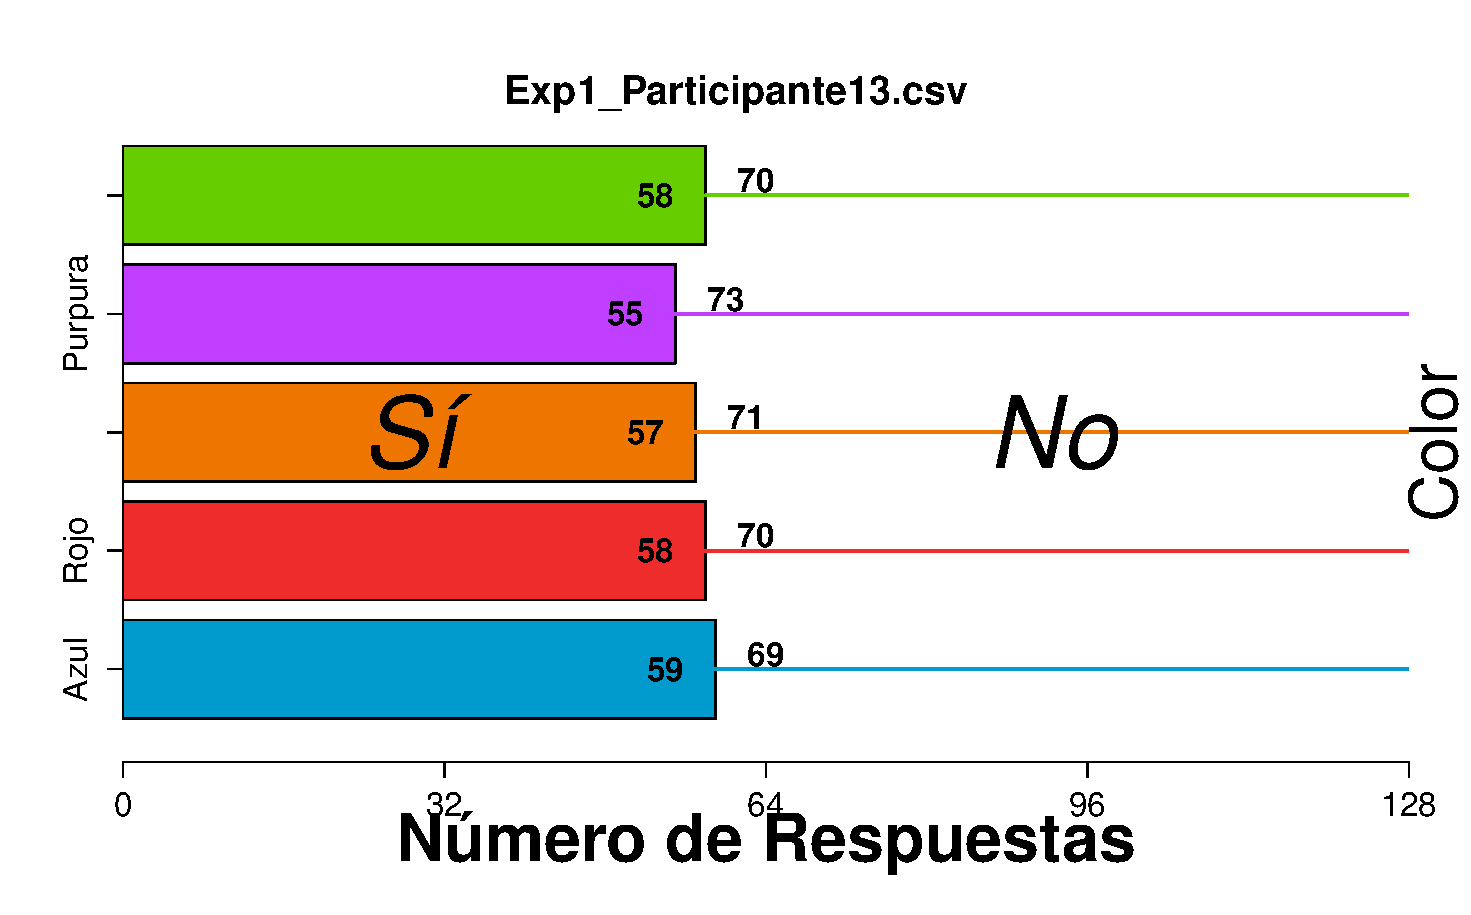
\includegraphics[width=0.40\textwidth]{Figures/BiasColor_Exp1_P13}
%\decoRule
\caption[Proporción de Respuestas 'Sí'/'No' por color; Ejemplo]{Se muestra el desempeño del Participante 14 del Experimento 1 en relación al color de los estímulos. En el panel izquierdo se muestra la relación entre el número de Hits obtenidos y el color de los estímulos, mientras que en el panel dercho se muestra la misma relación para las Falsas alarmas.}
\label{fig:BiasCol_E1_P13}
\end{figure}

Las Figuras~\ref{fig:BiasCol_E1} y ~\ref{fig:BiasColor_E2} muestran las gráficas correspondientes al resto de los participantes en los Experimentos 1 y 2, respectivamente. 

\end{itemize}













\section{Control 4: Evidencia del Efecto Espejo}

Una vez revisada la ejecución de los participantes en aras de asegurar la pertinencia del diseño experimental a la luz de las respuestas observadas, y antes de pasar al análisis estadístico formal de los datos, se realizó una evaluación visual preliminar de los mismos en búsqueda de la presencia del Efecto Espejo en las tareas propuestas.

\begin{itemize}
\item Patrón de Hits y Falsas Alarmas (Tarea binaria).

La Figura~\ref{fig:MirrorRate_E2_P4} muestra la frecuencia absoluta de Hits y Falsas Alarmas obtenidas por el Participante 4 en el Experimento 2, en cada una de las condiciones de dificultad puestas a prueba. Como se puede apreciar, este participante muestra claramente el patrón de respuestas identificado como parte del Efecto Espejo en la literatura, siendo que en la condición fácil (A) tiene más aciertos (Hits en AS > Hits en BS) y menos errores (Falsas Alarmas en AN < Falsas Alarmas en BN). Estas discrepancias en el desempeño del participante son consistentes con la idea de que existe una distribución de señal y una distribución de ruido por cada condición de dificultad, que se distribuye en el espacio de elección como un reflejo que se aleja en ambas direcciones, bajo el supuesto de que los participantes están respondiendo a la tarea utilizando un único criterio de elección y que ignoran la existencia de más de un 'tipo de estímulo'.\\

\begin{figure}[th]
\centering
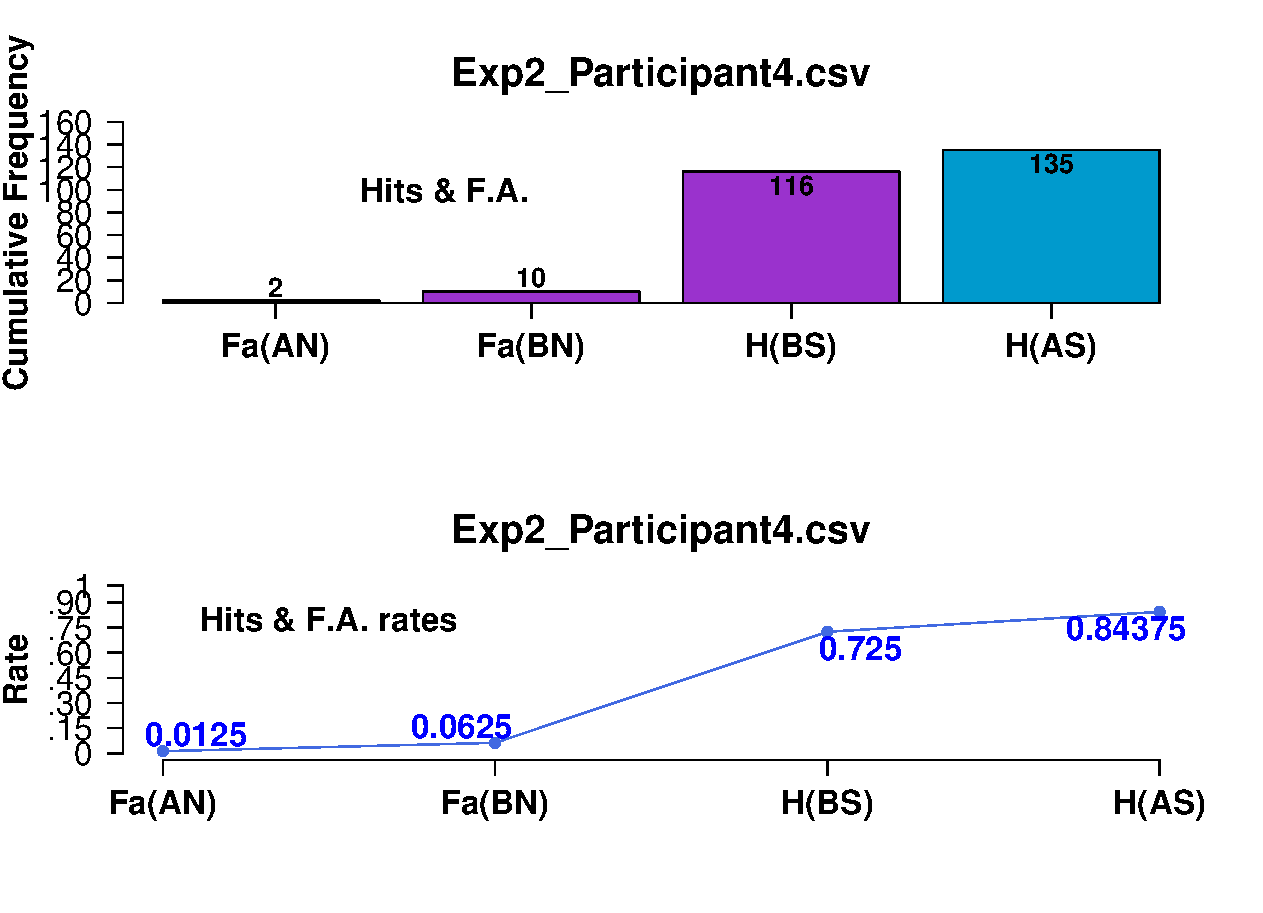
\includegraphics[width=0.60\textwidth]{Figures/MirrorRate_Exp2_P4}
%\decoRule
\caption[Diferencias entre Hits y Falsas Alarmas por Condición; Ejemplo]{Se muestra el desempeño del Participante 14 del Experimento 1 en relación al color de los estímulos. En el panel izquierdo se muestra la relación entre el número de Hits obtenidos y el color de los estímulos, mientras que en el panel derecho se muestra la misma relación para las Falsas alarmas.}
\label{fig:MirrorRate_E2_P4}
\end{figure}

La comparación entre los Hits y Falsas Alarmas de cada condición de dificultad para el resto de los participantes de los Experimentos 1 y 2, se muestran en las Figuras~\ref{fig:MRate_E1} y ~\ref{fig:MRate_E2}.\\

\item Patrón de Puntaje de Confianza (Escala de Confianza).

La Figura~\ref{fig:MirrorRating_E1_P10} muestra el promedio de los puntajes de confianza asignados por el Participante 10 del Experimento 1 a los estímulos pertenecientes a cada una de las condiciones de dificultad construidas, separando para cada caso los ensayos con ruido y señal. En la figura puede apreciarse con claridad una tendencia ascendente que coincide con el patrón reportado en estudios de Memoria de Reconocimiento.\\

\begin{figure}[th]
\centering
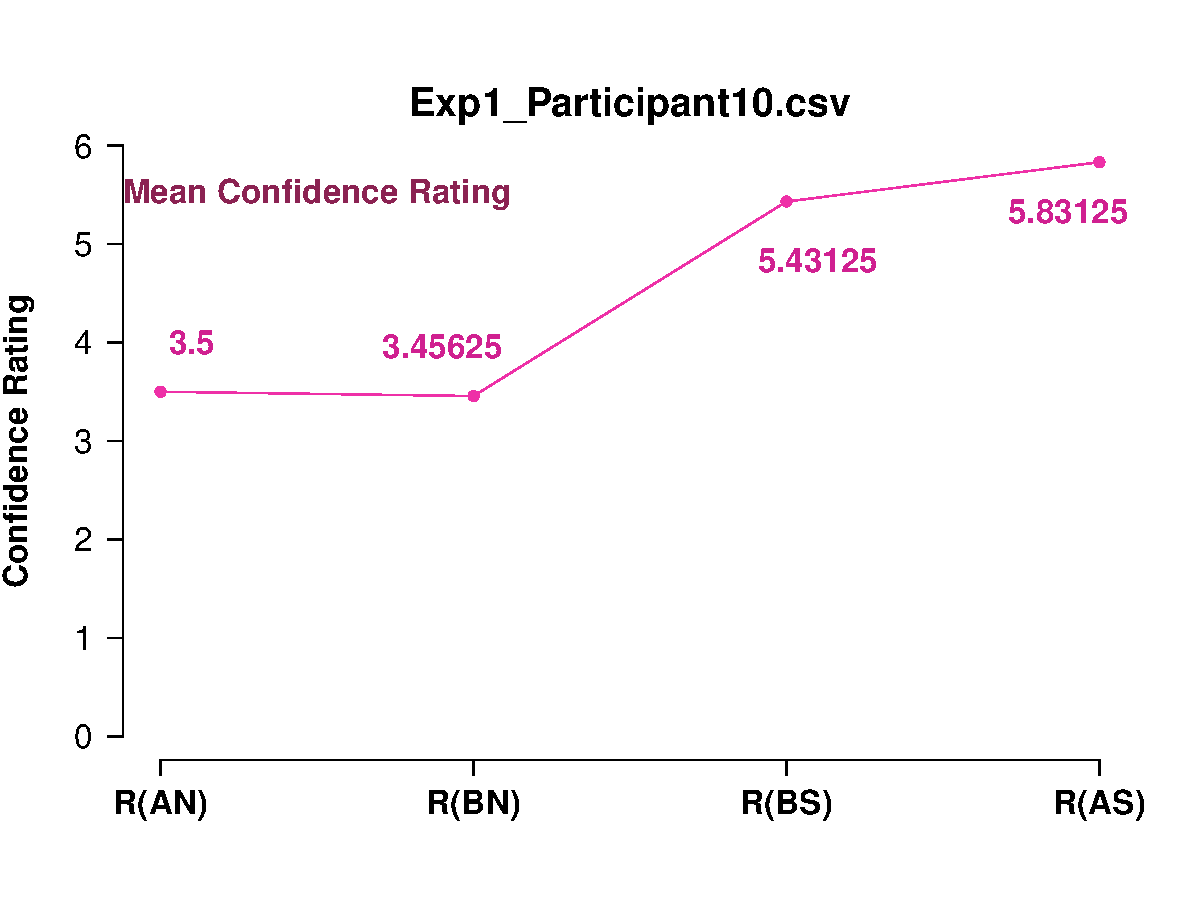
\includegraphics[width=0.60\textwidth]{Figures/MirrorRating_Exp1_P10}
%\decoRule
\caption[Comparación entre Puntajes de Confianza asignados por Condición; Ejemplo]{Se muestra el desempeño del Participante 14 del Experimento 1 en relación al color de los estímulos. En el panel izquierdo se muestra la relación entre el número de Hits obtenidos y el color de los estímulos, mientras que en el panel derecho se muestra la misma relación para las Falsas alarmas.}
\label{fig:MirrorRating_E1_P10}
\end{figure}

La comparación entre los puntajes de confianza asignados a cada grupo de estímulos por el resto de los participantes en los Experimentos 1 y 2, se presentan en las Figuras~\ref{fig:MERating_E1} y ~\ref{fig:MERating_E2}.\\

\end{itemize}




















%\begin{figure}[th]
%\centering
%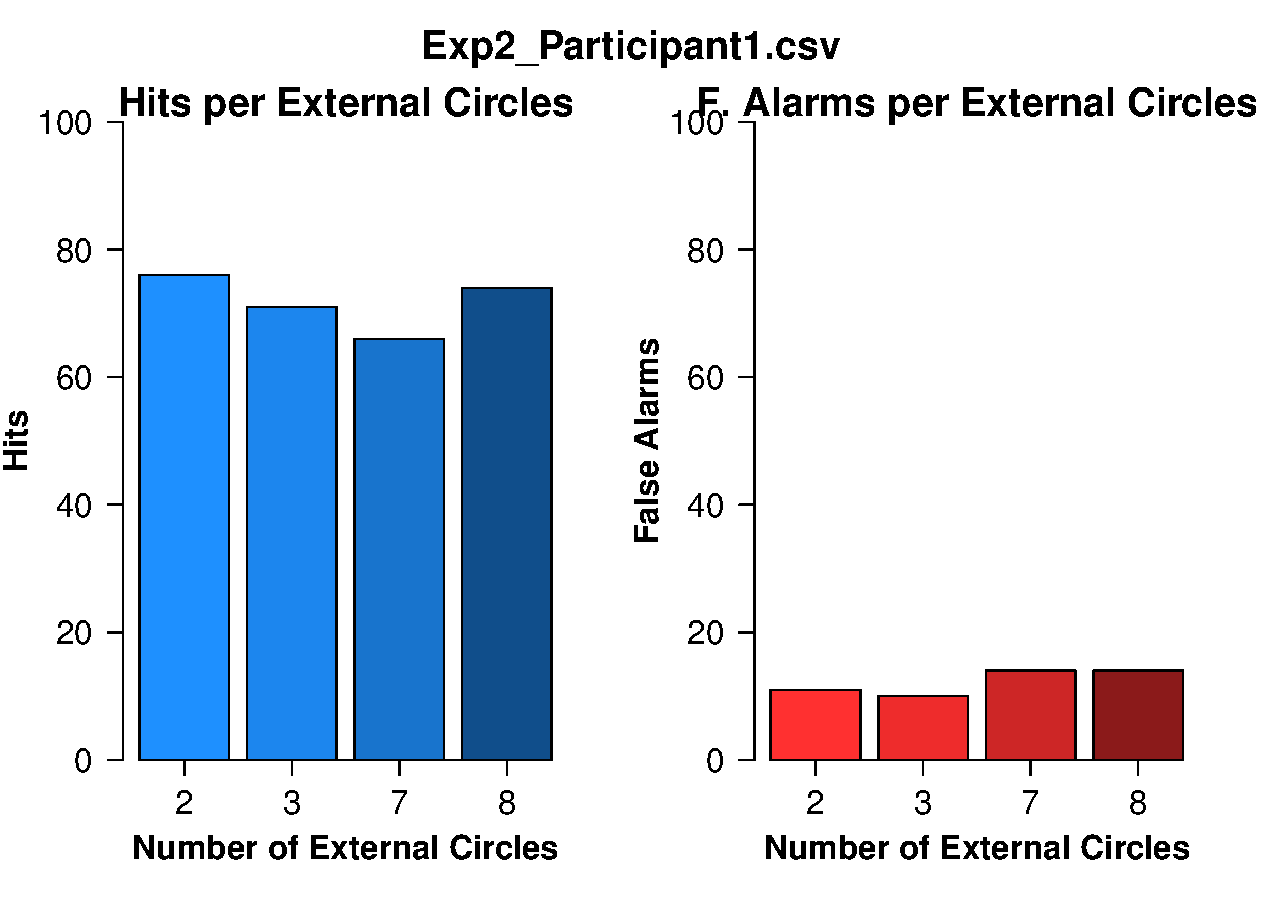
\includegraphics[width=0.30\textwidth]{Figures/Numero_Exp2_P1} 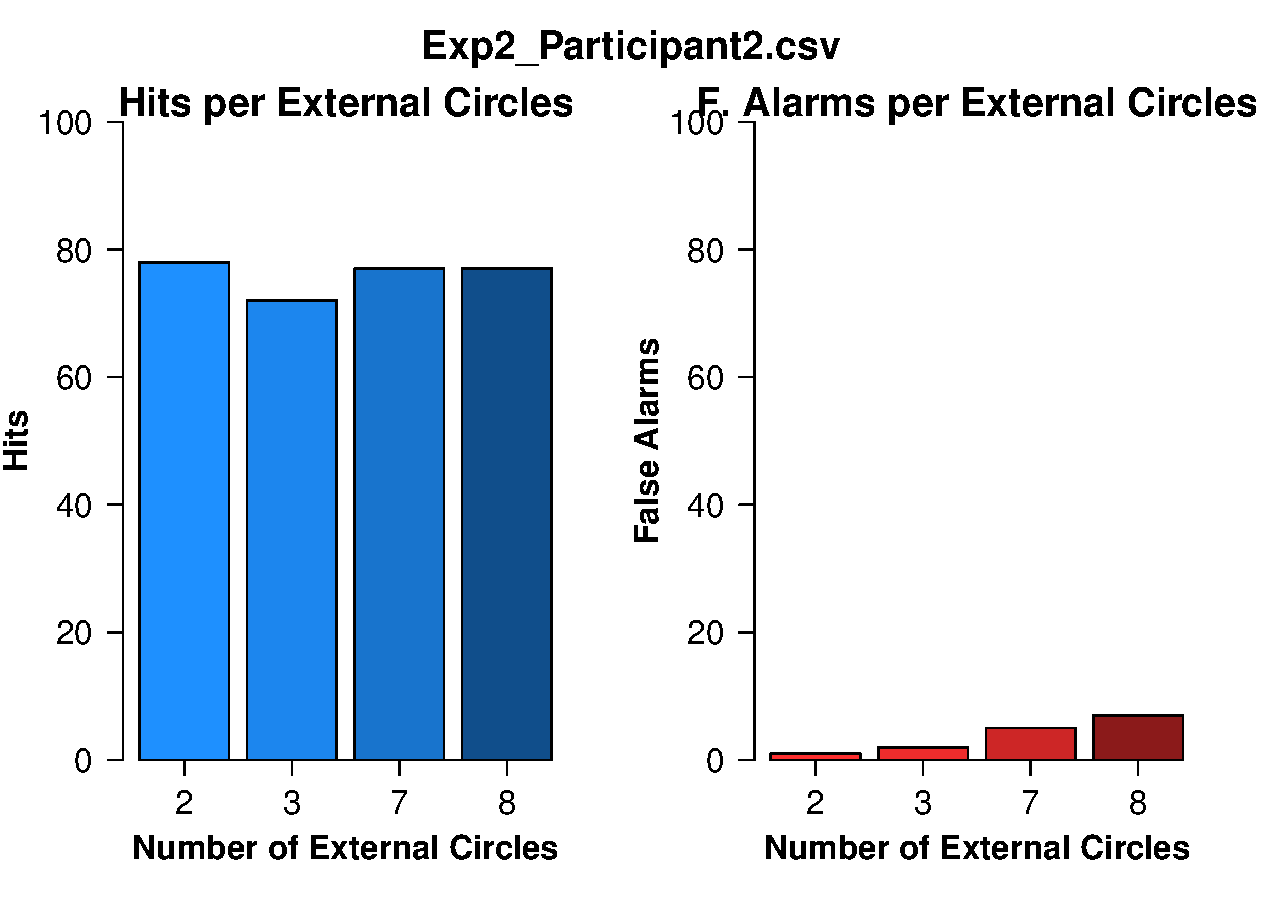
\includegraphics[width=0.30\textwidth]{Figures/Numero_Exp2_P2} 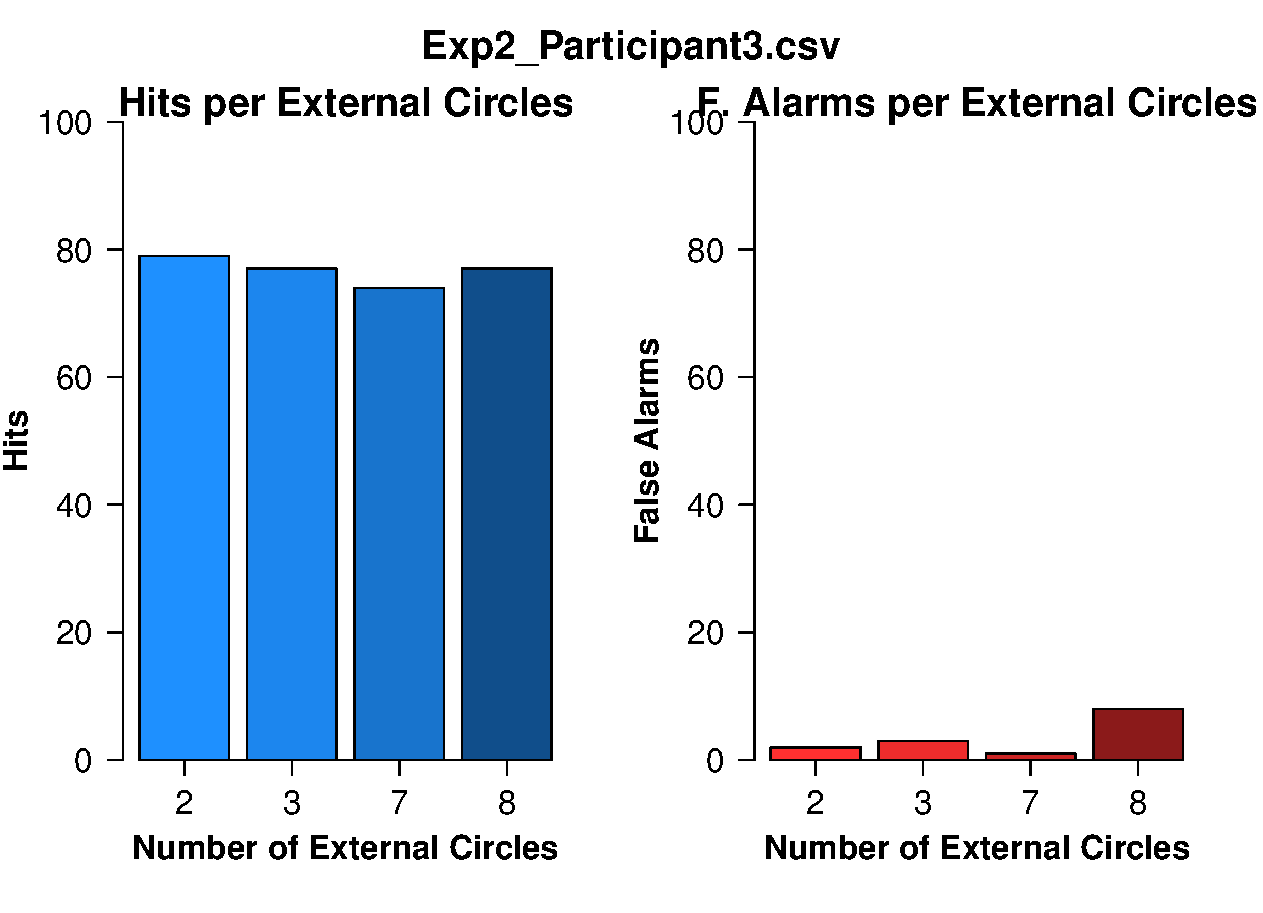
\includegraphics[width=0.30\textwidth]{Figures/Numero_Exp2_P3}
%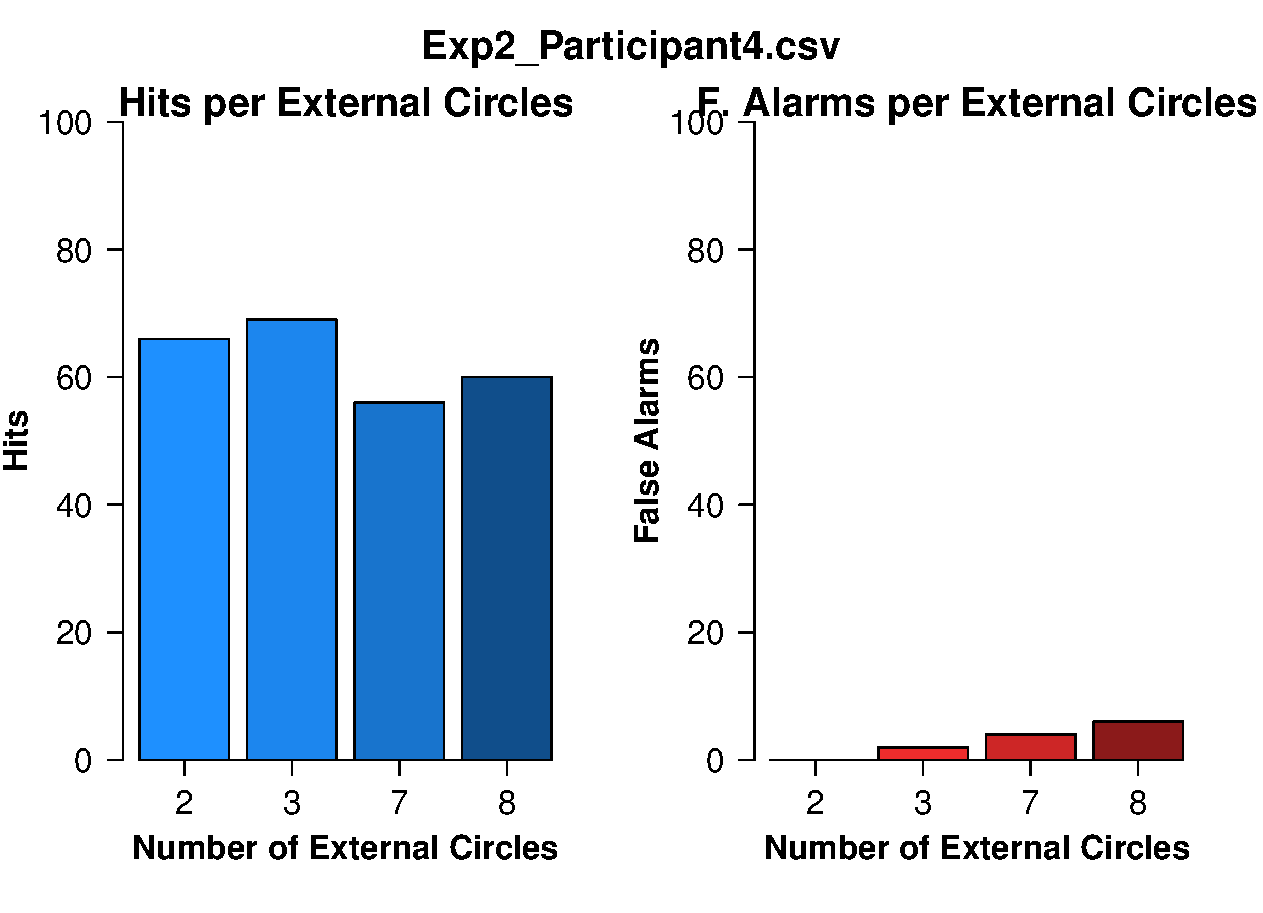
\includegraphics[width=0.30\textwidth]{Figures/Numero_Exp2_P4} 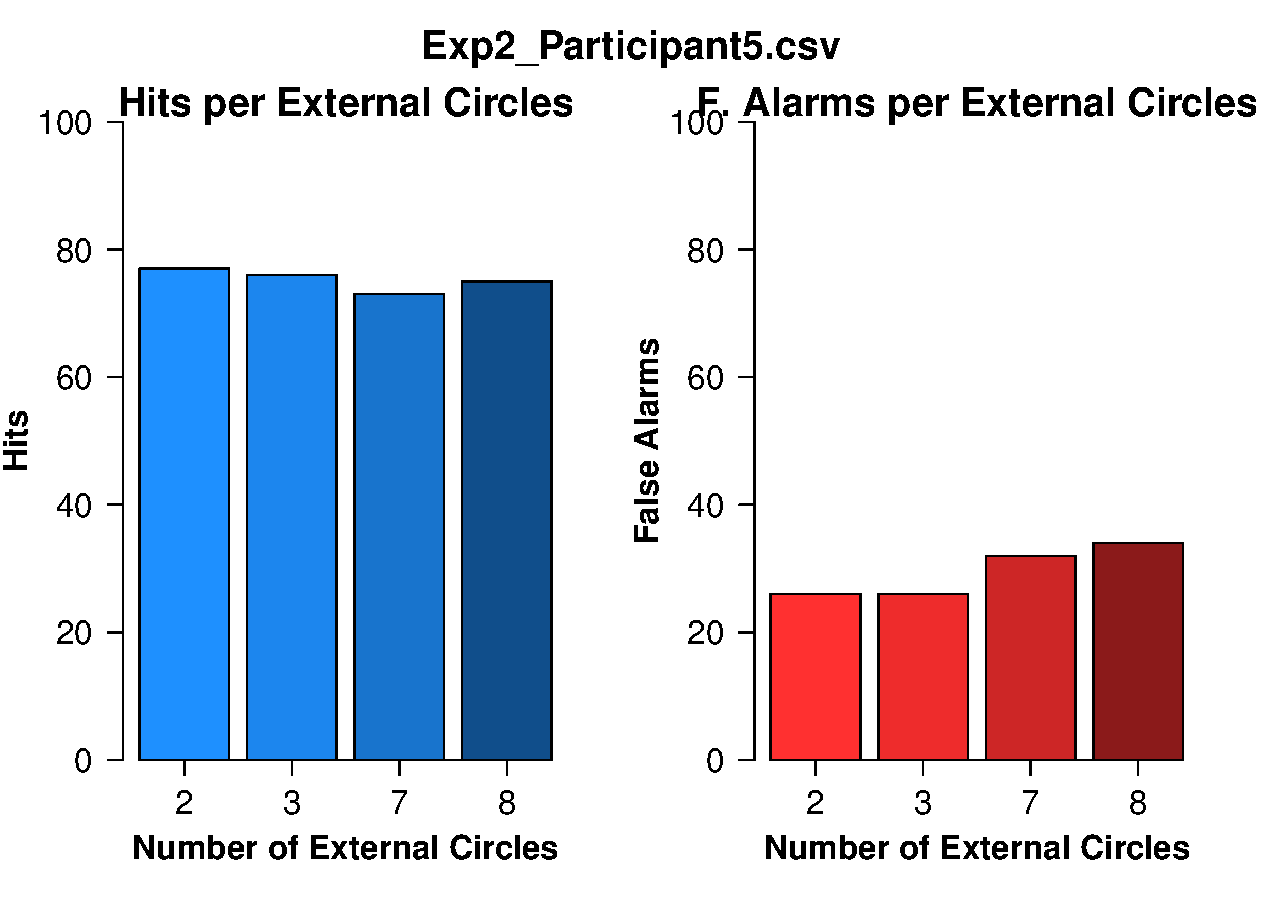
\includegraphics[width=0.30\textwidth]{Figures/Numero_Exp2_P5} 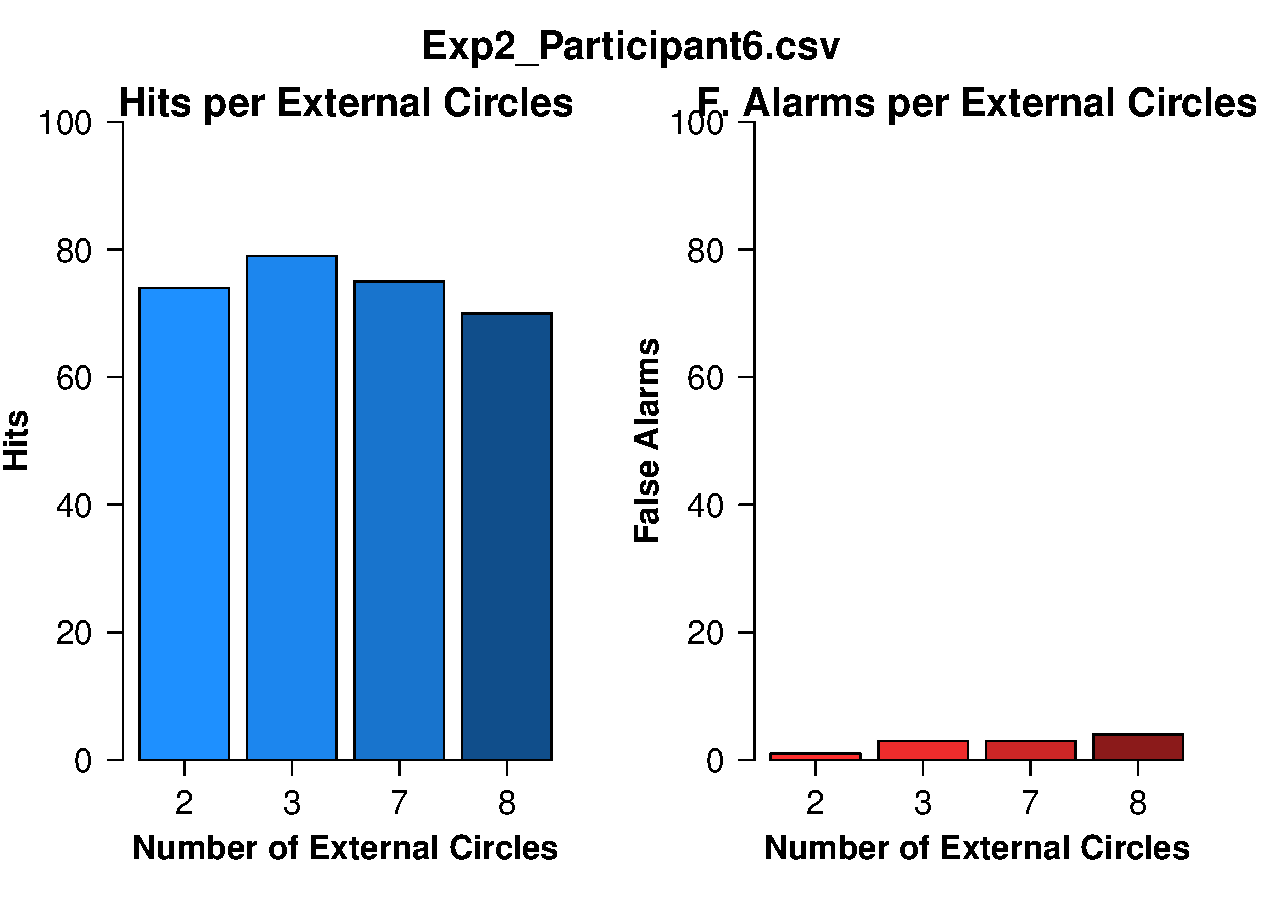
\includegraphics[width=0.30\textwidth]{Figures/Numero_Exp2_P6}
%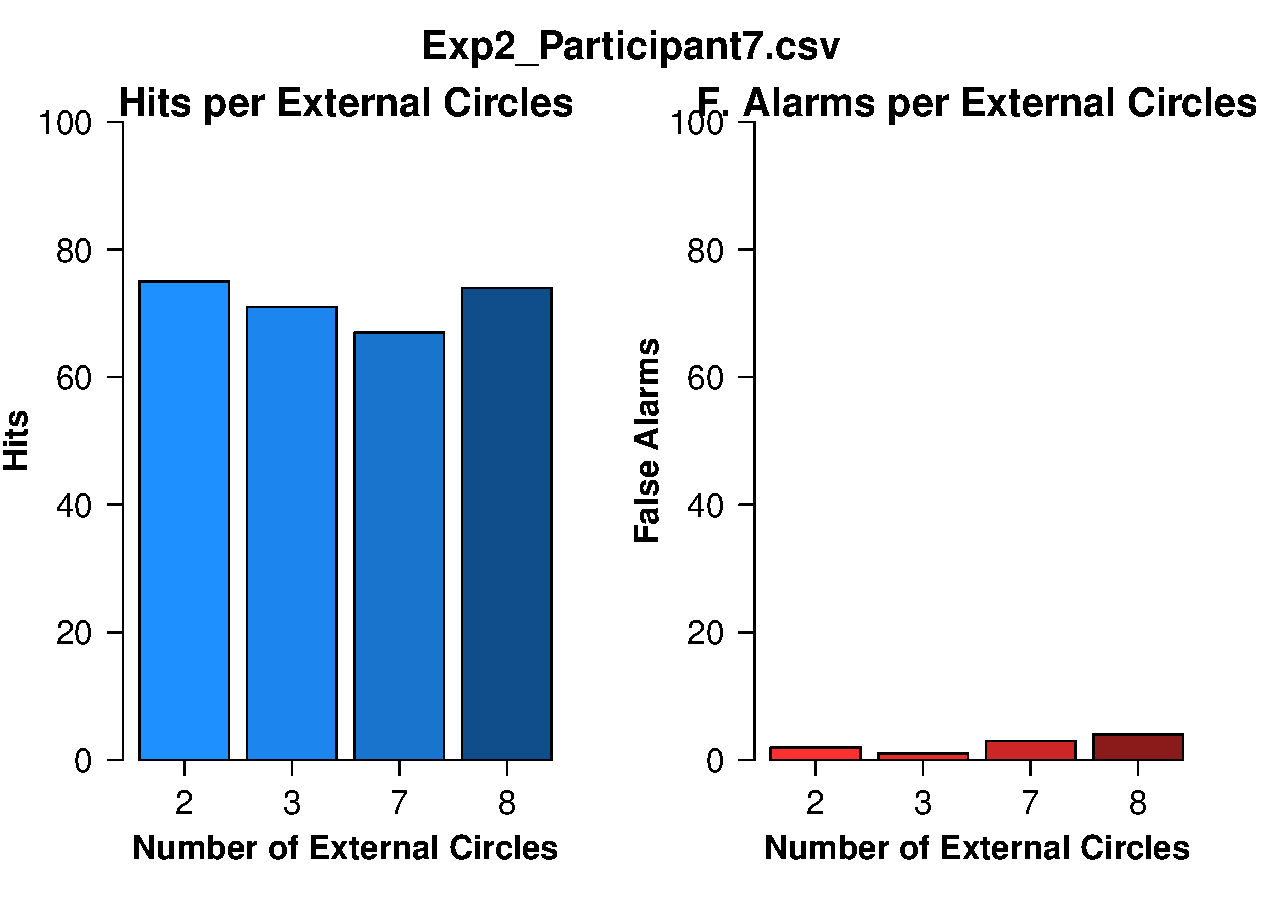
\includegraphics[width=0.30\textwidth]{Figures/Numero_Exp2_P7} 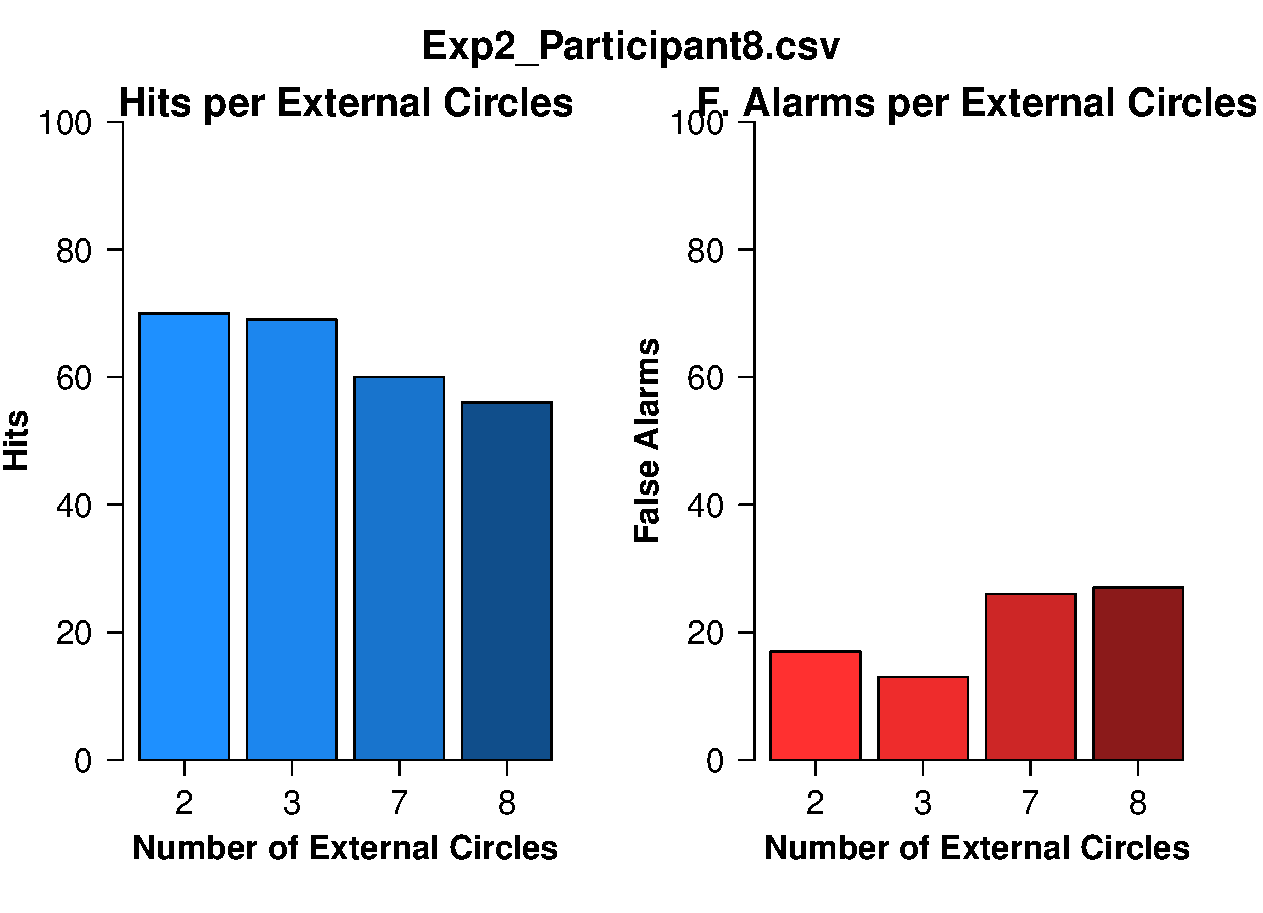
\includegraphics[width=0.30\textwidth]{Figures/Numero_Exp2_P8} 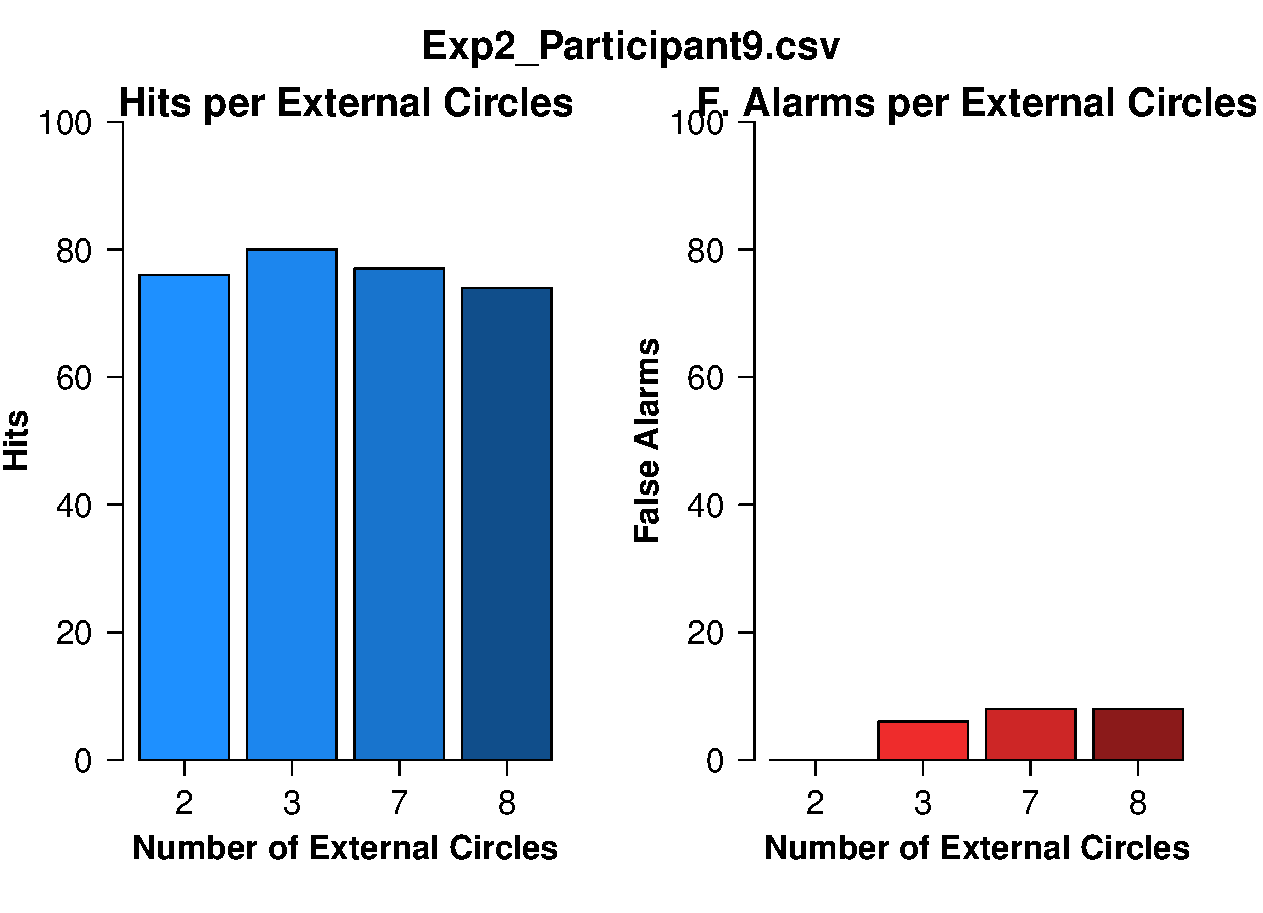
\includegraphics[width=0.30\textwidth]{Figures/Numero_Exp2_P9}
%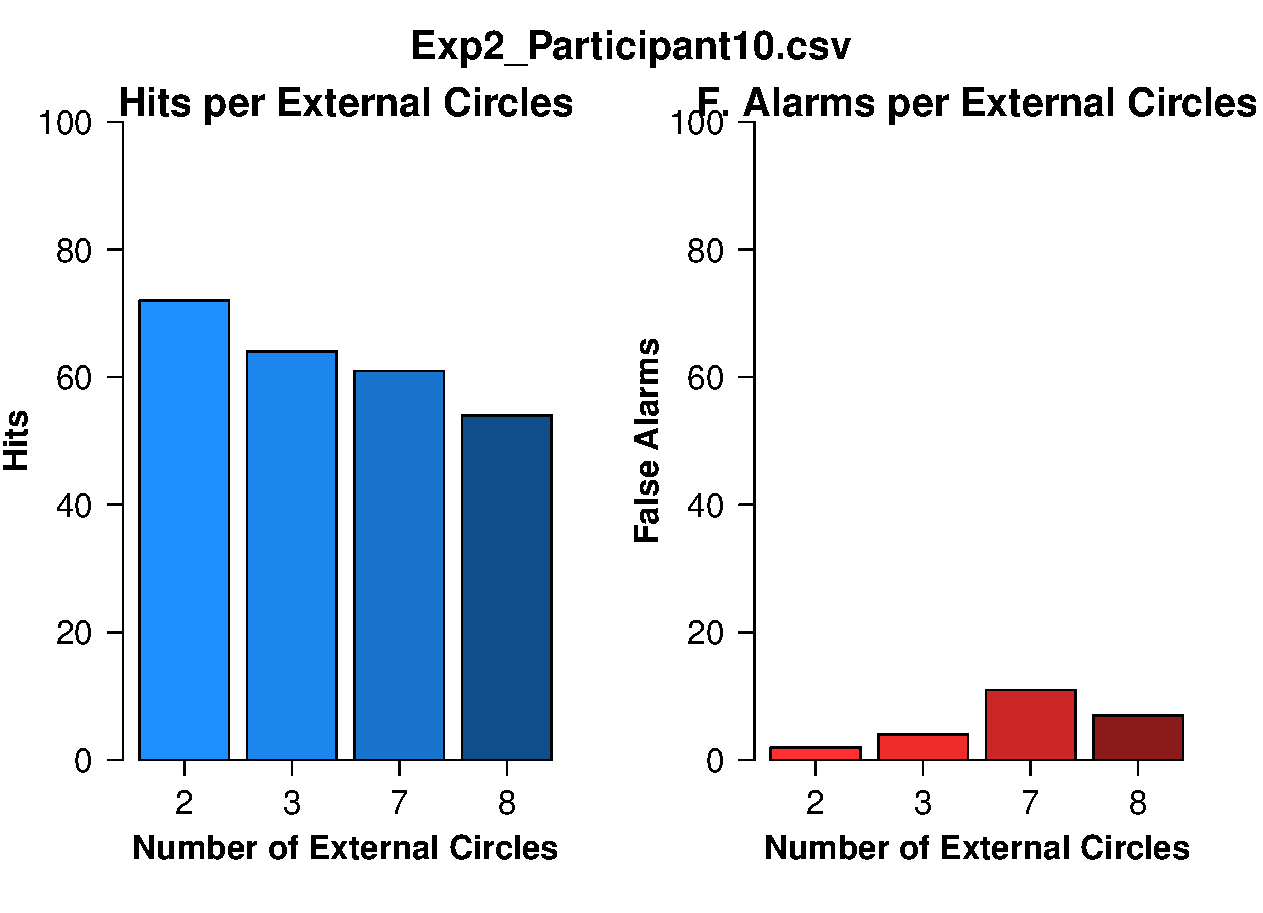
\includegraphics[width=0.30\textwidth]{Figures/Numero_Exp2_P10} 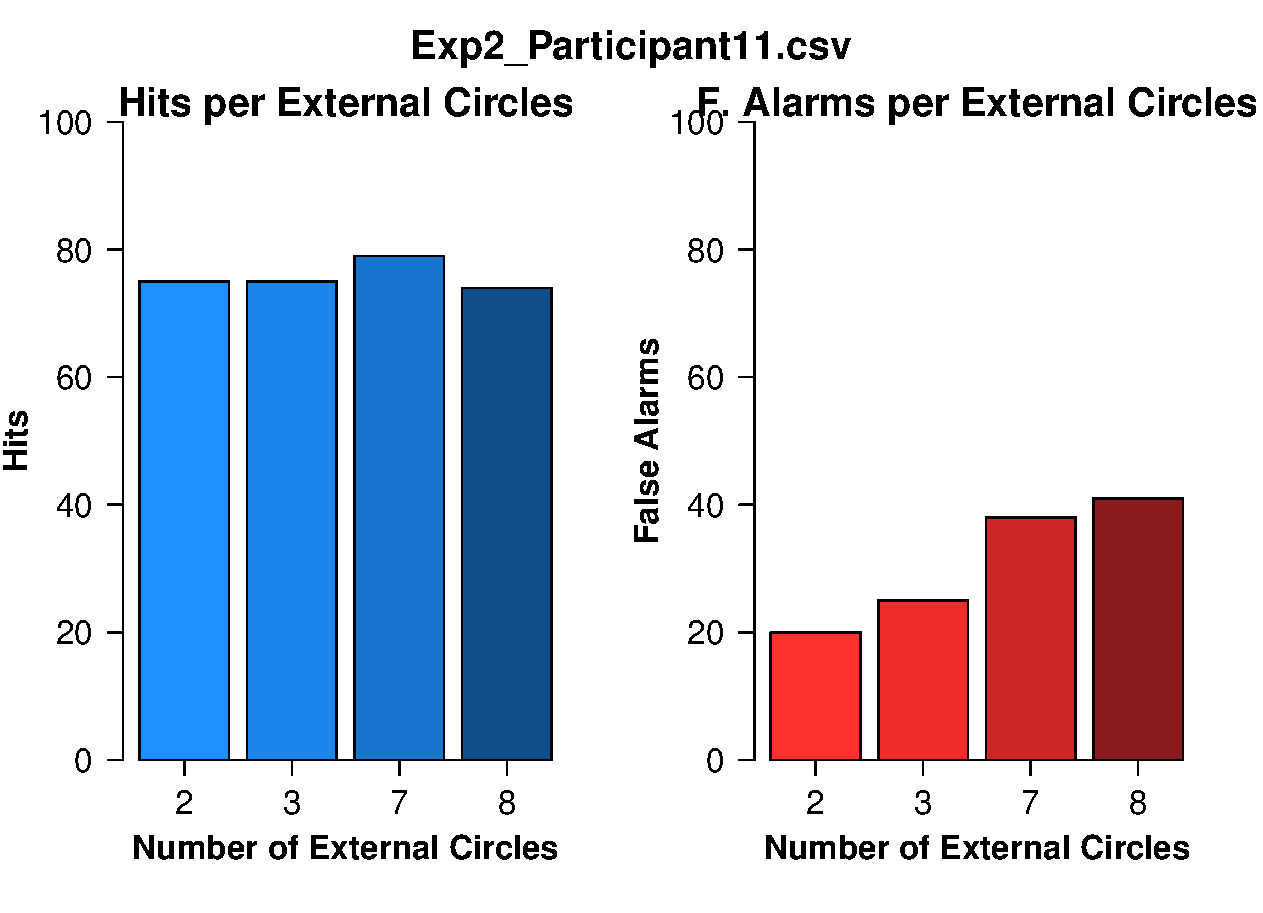
\includegraphics[width=0.30\textwidth]{Figures/Numero_Exp2_P11} 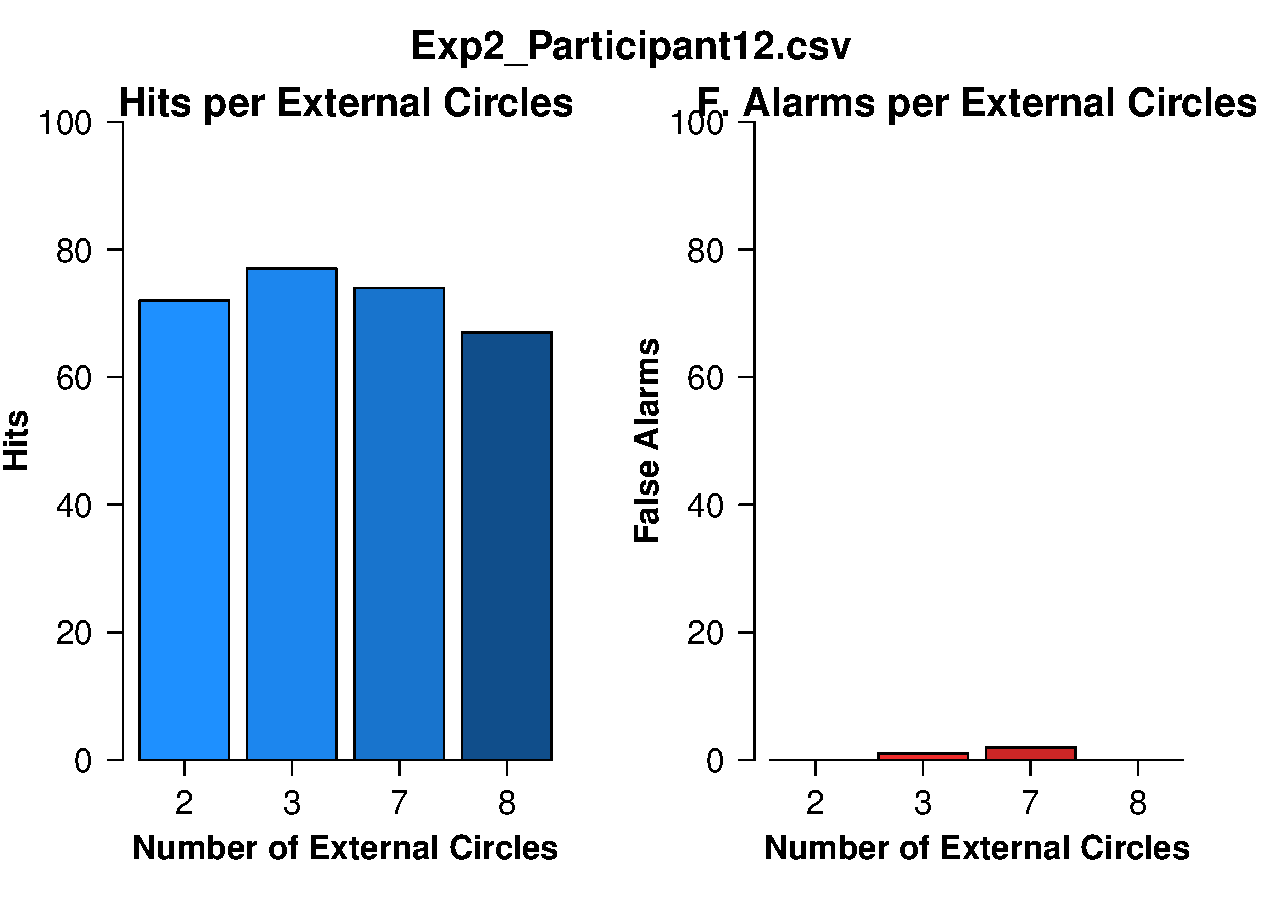
\includegraphics[width=0.30\textwidth]{Figures/Numero_Exp2_P12}
%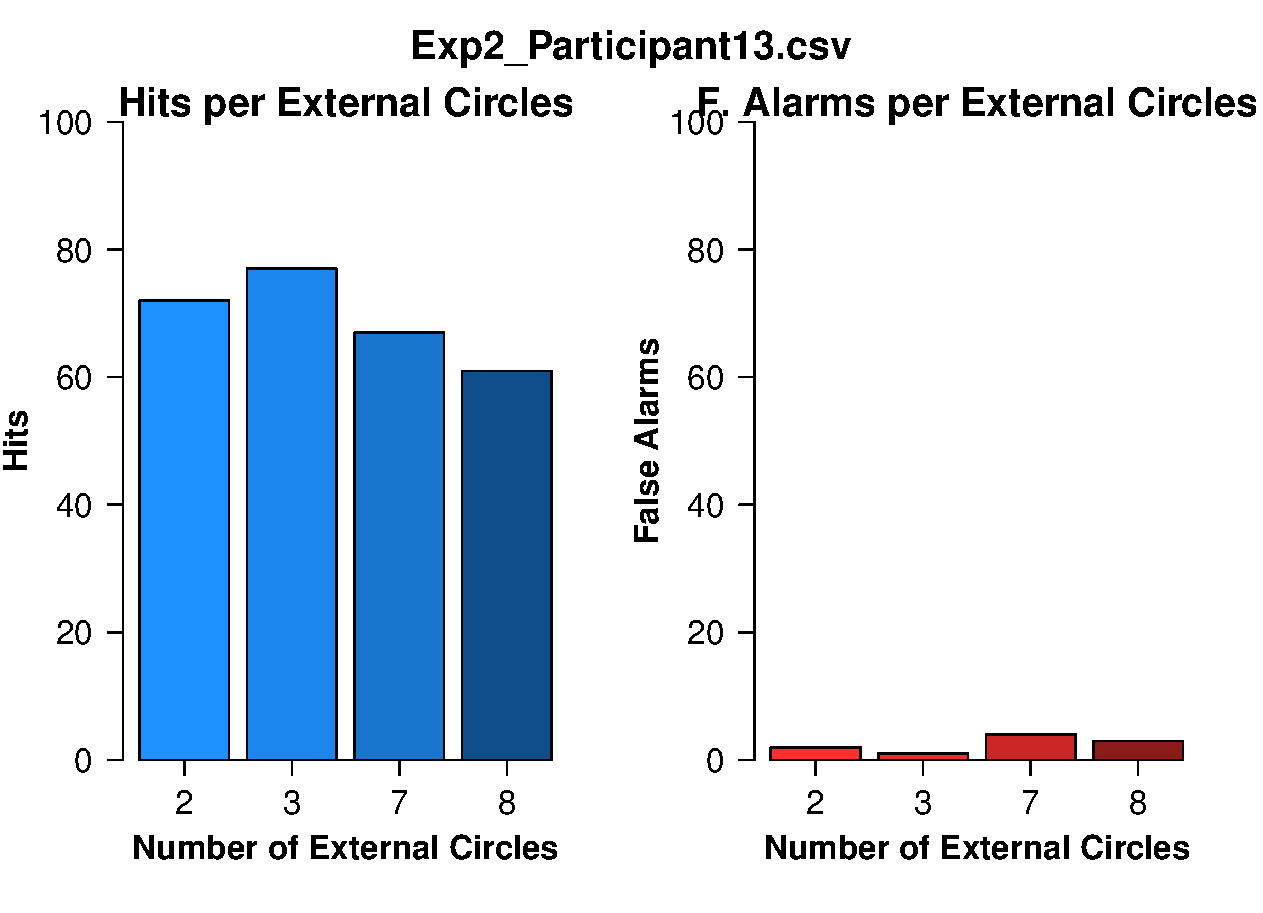
\includegraphics[width=0.30\textwidth]{Figures/Numero_Exp2_P13} 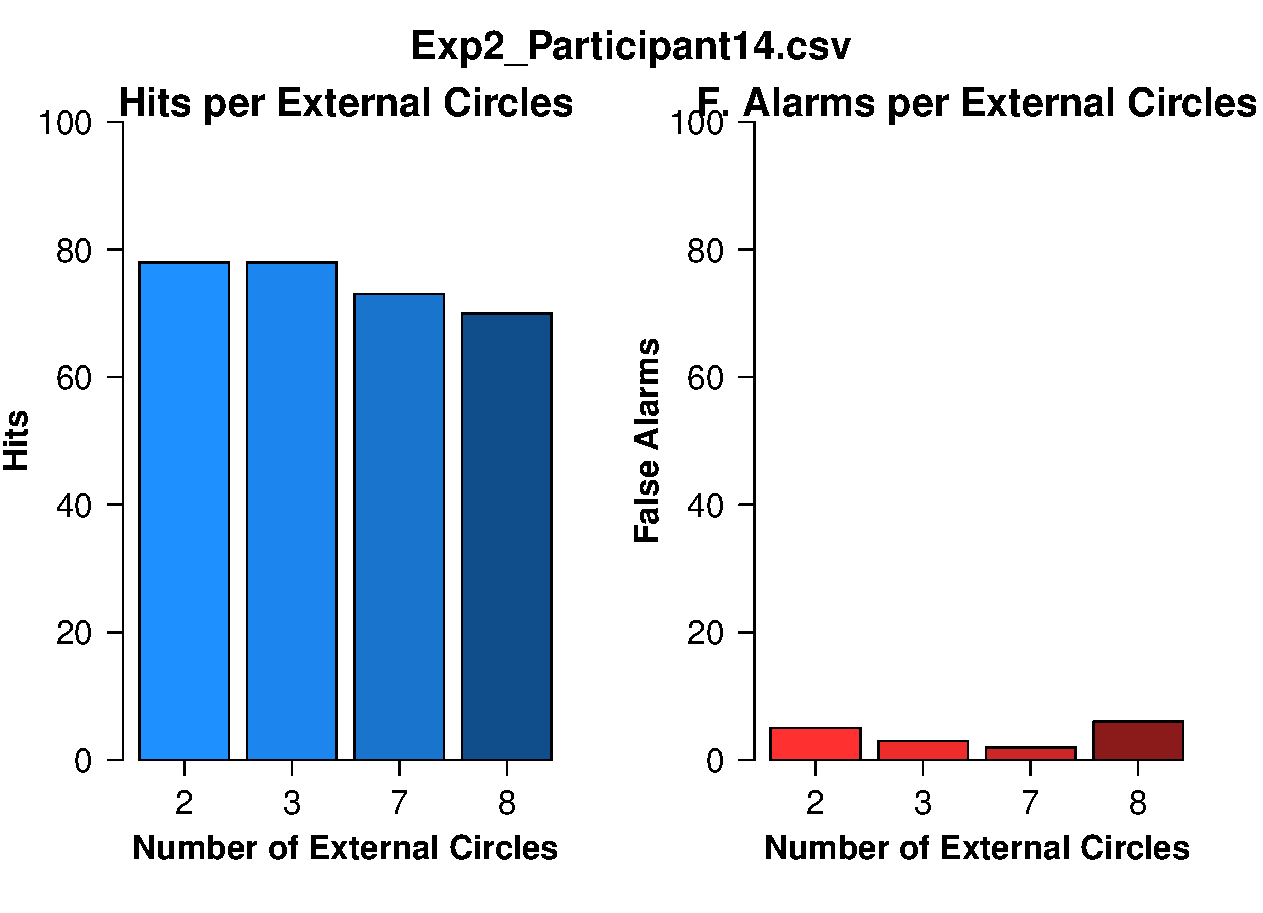
\includegraphics[width=0.30\textwidth]{Figures/Numero_Exp2_P14} 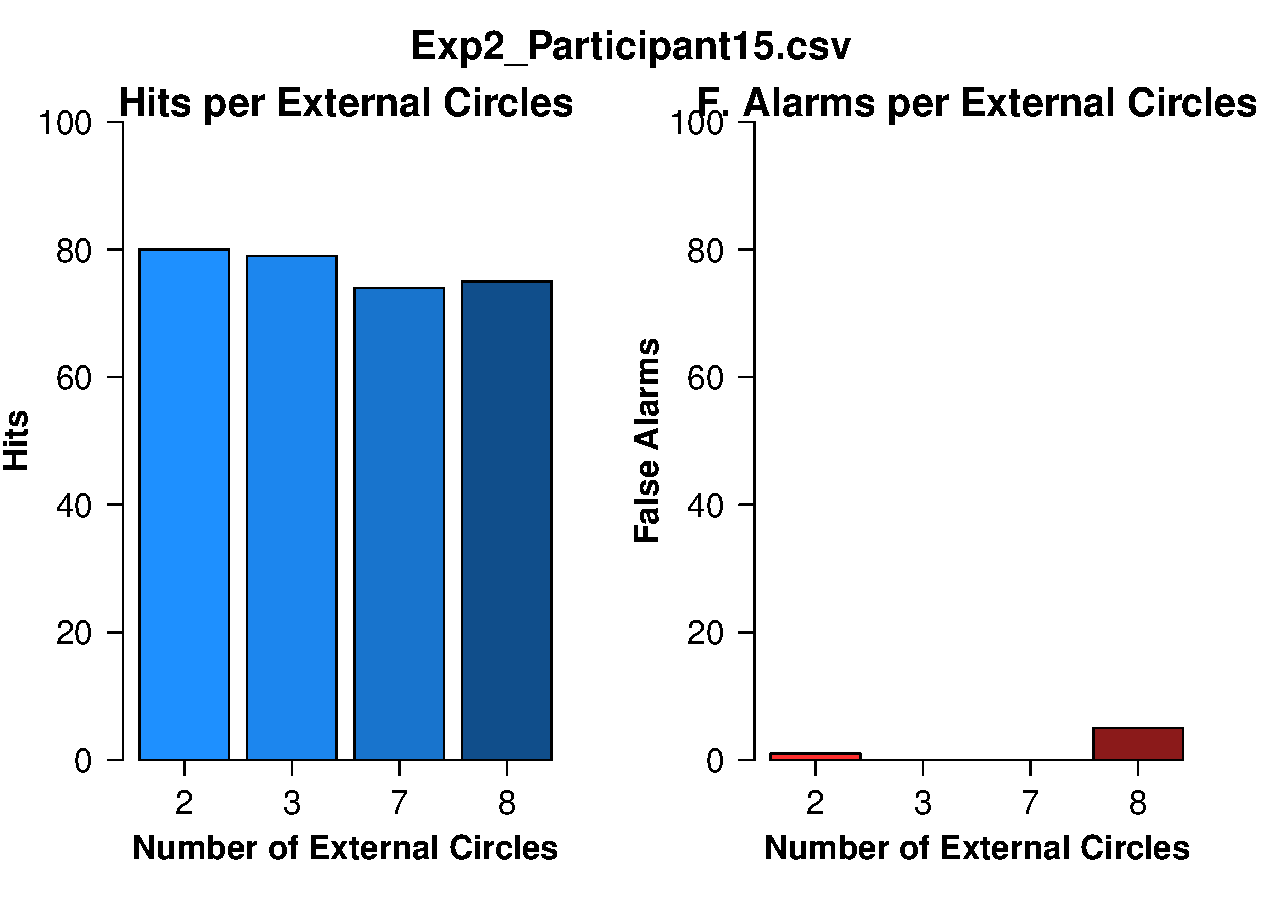
\includegraphics[width=0.30\textwidth]{Figures/Numero_Exp2_P15}
%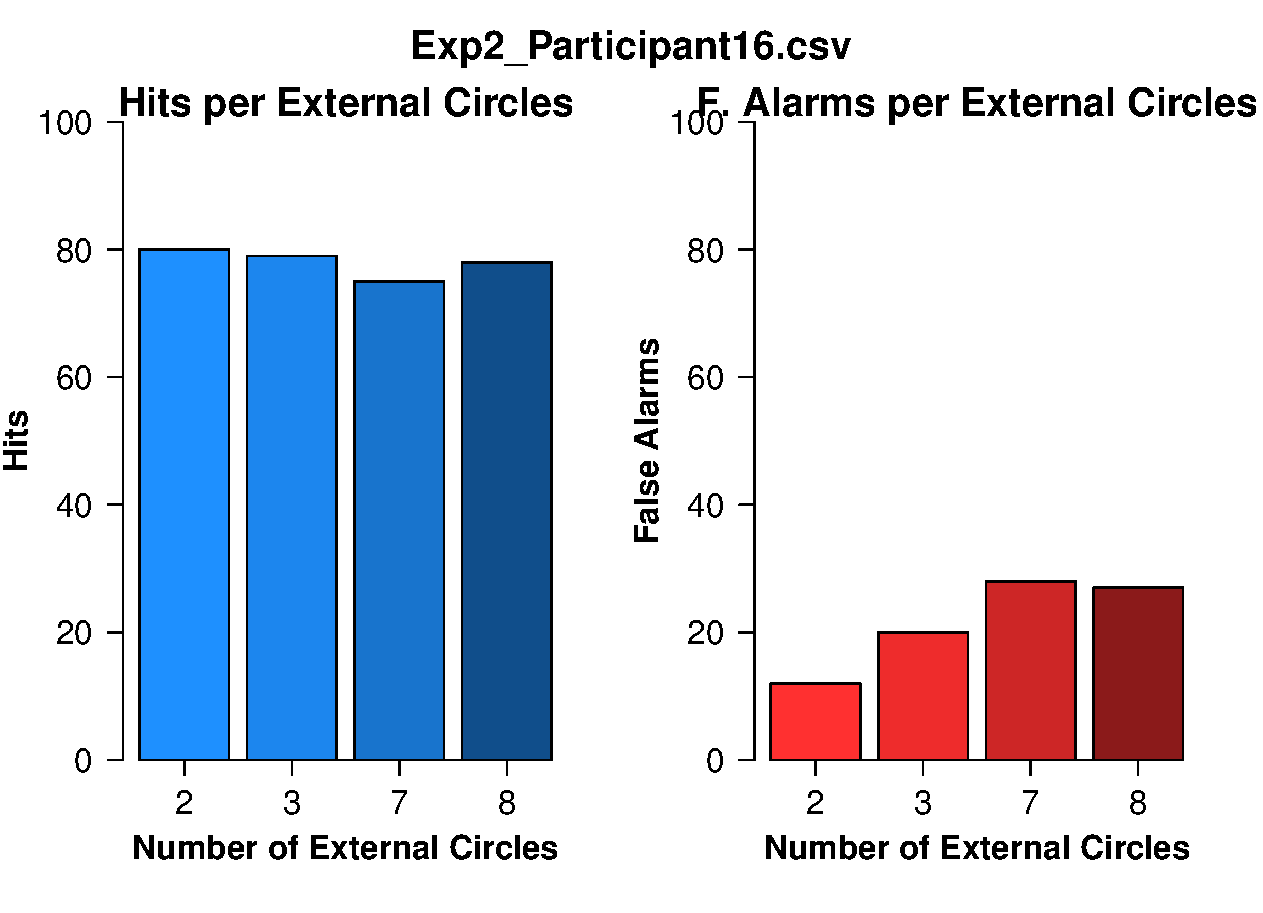
\includegraphics[width=0.30\textwidth]{Figures/Numero_Exp2_P16} 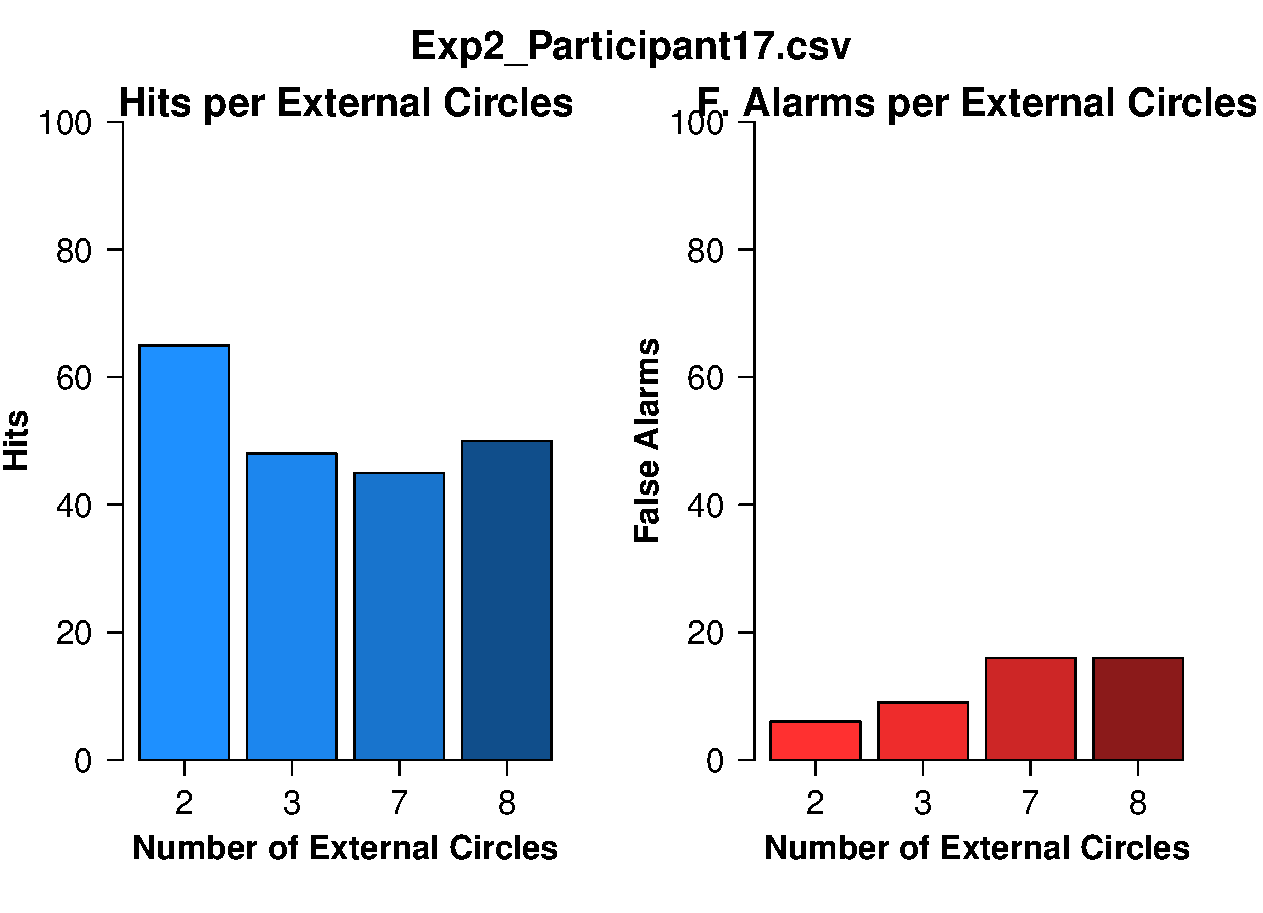
\includegraphics[width=0.30\textwidth]{Figures/Numero_Exp2_P17} 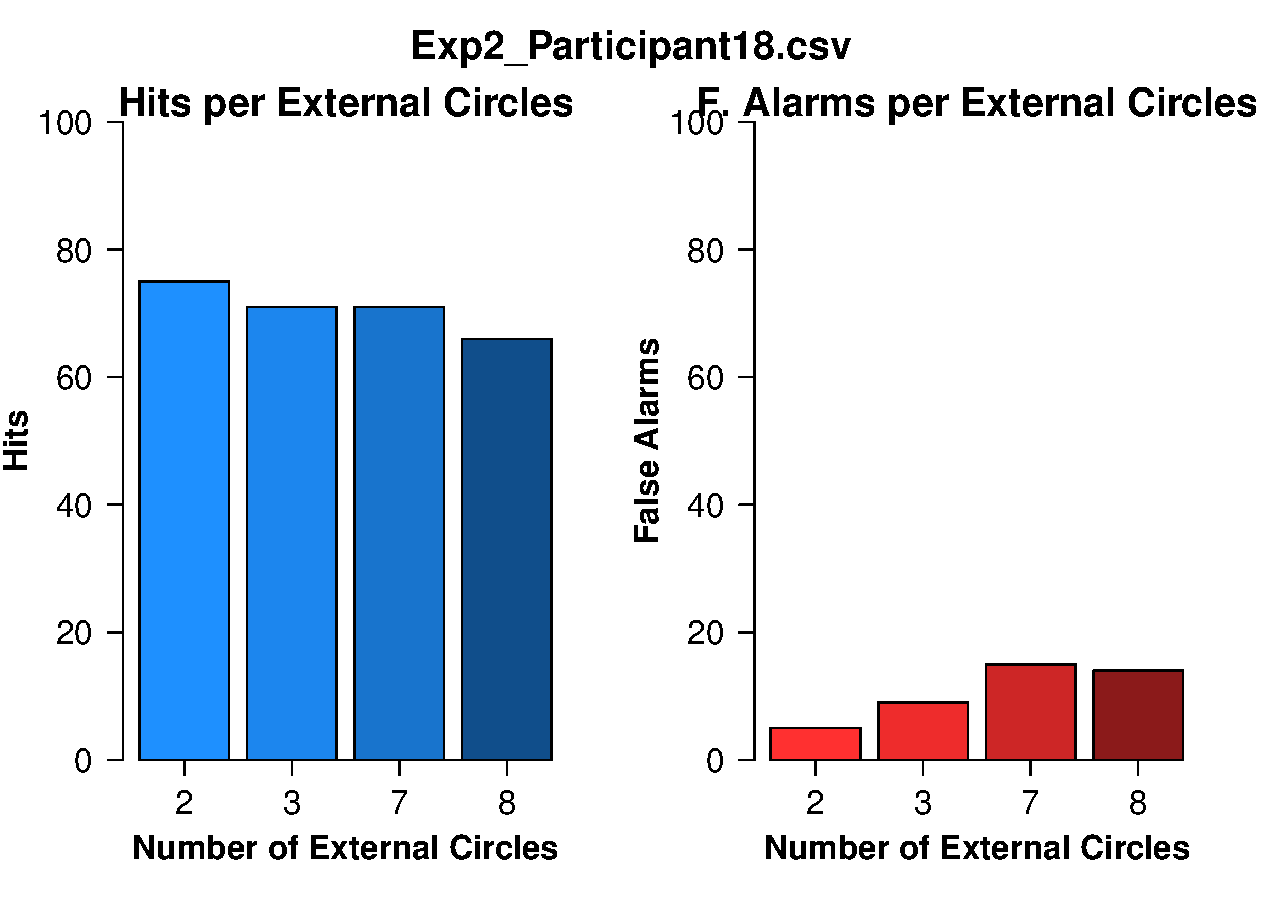
\includegraphics[width=0.30\textwidth]{Figures/Numero_Exp2_P18}
%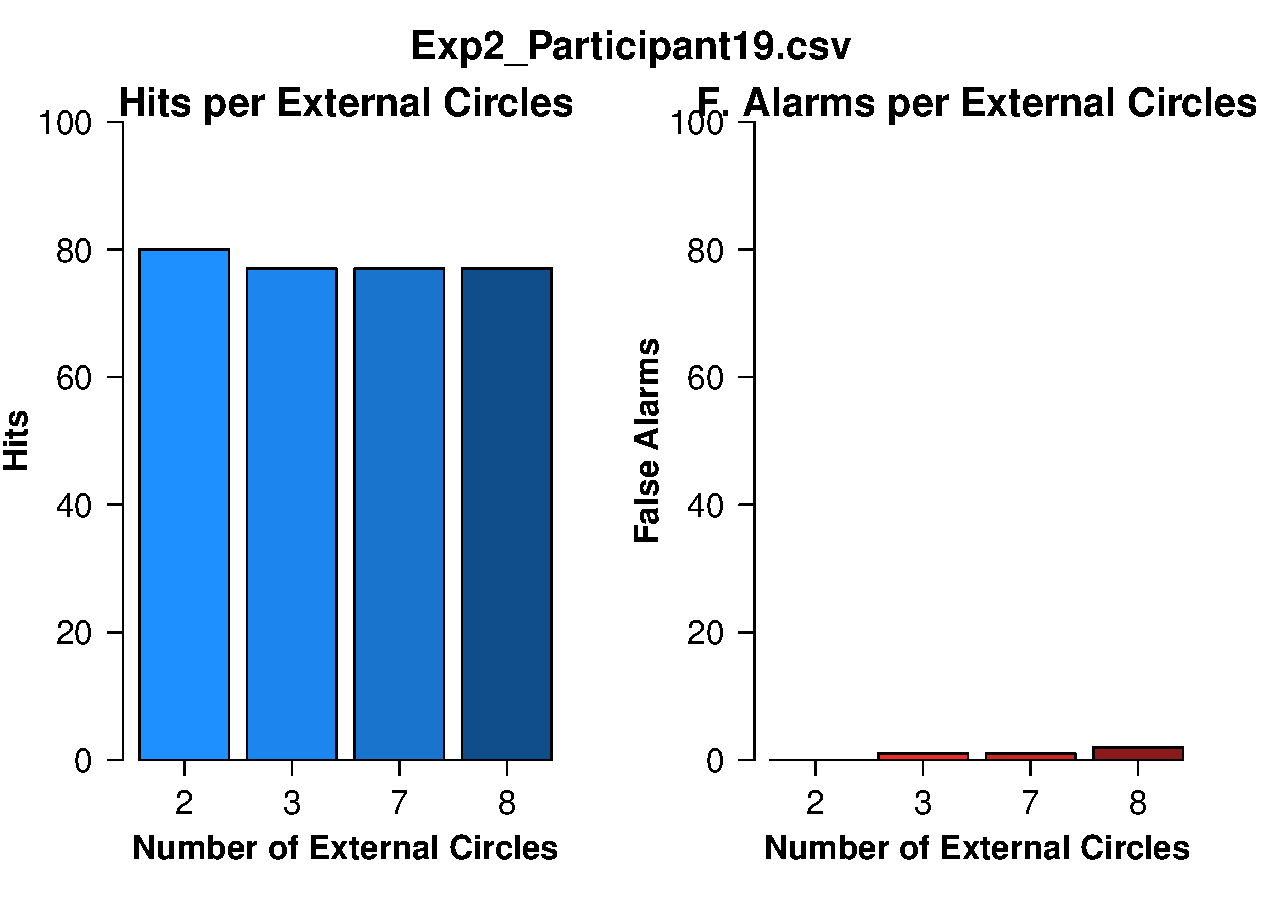
\includegraphics[width=0.30\textwidth]{Figures/Numero_Exp2_P19} 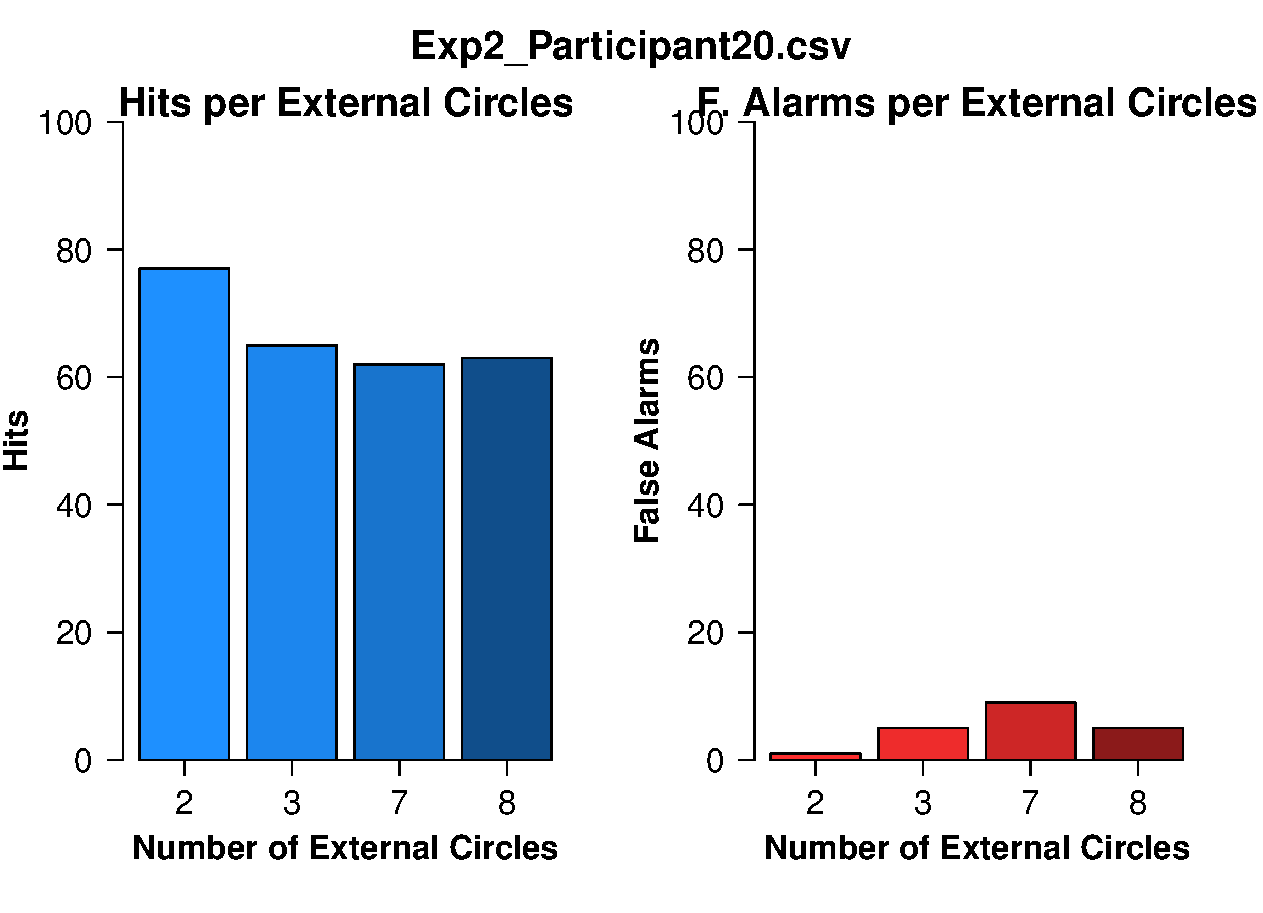
\includegraphics[width=0.30\textwidth]{Figures/Numero_Exp2_P20} 
%%\decoRule
%\caption[Numero_Exp2]{Efecto del Numero de Circulos Externos (Experimento 2).}
%\label{fig:Numero_E2}
%\end{figure}

\begin{figure}[th]
\centering
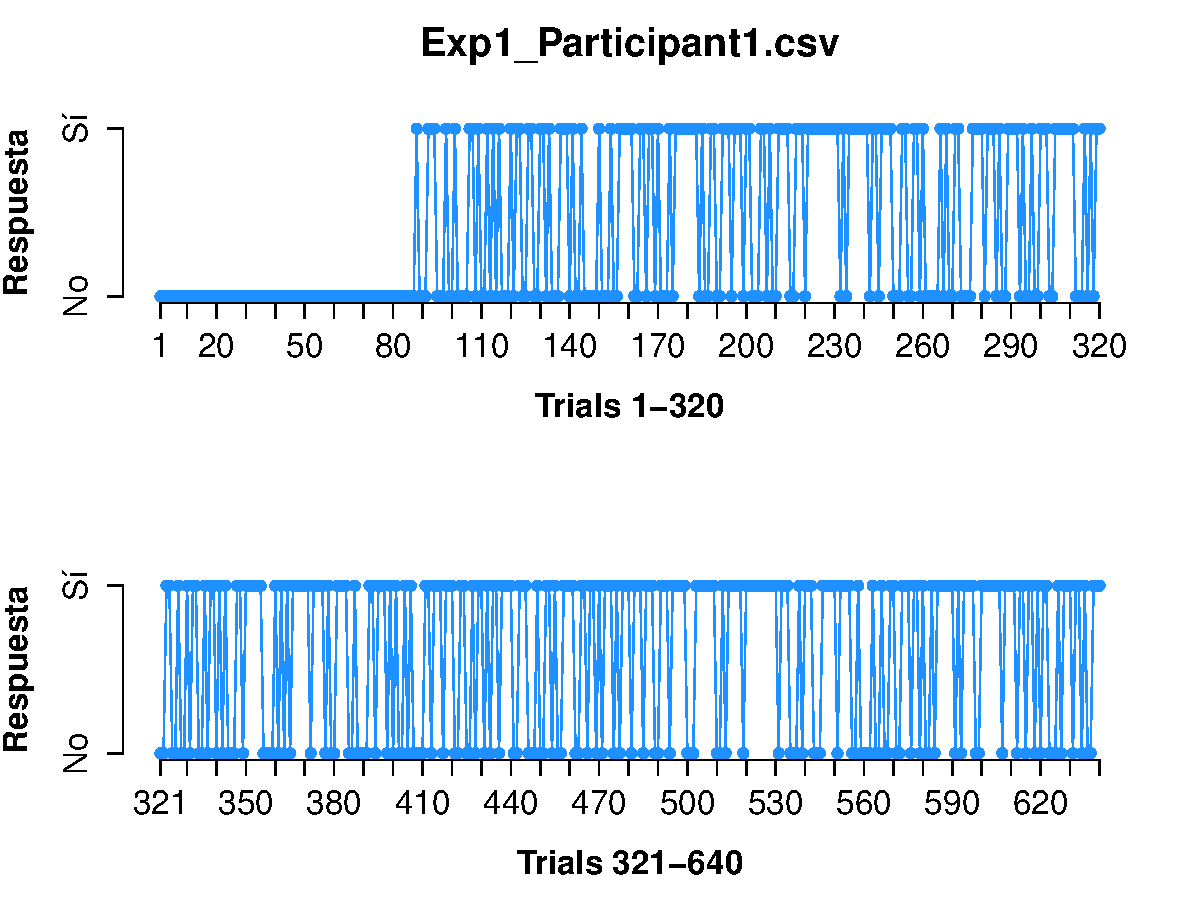
\includegraphics[width=0.30\textwidth]{Figures/Response_Exp1_P1} 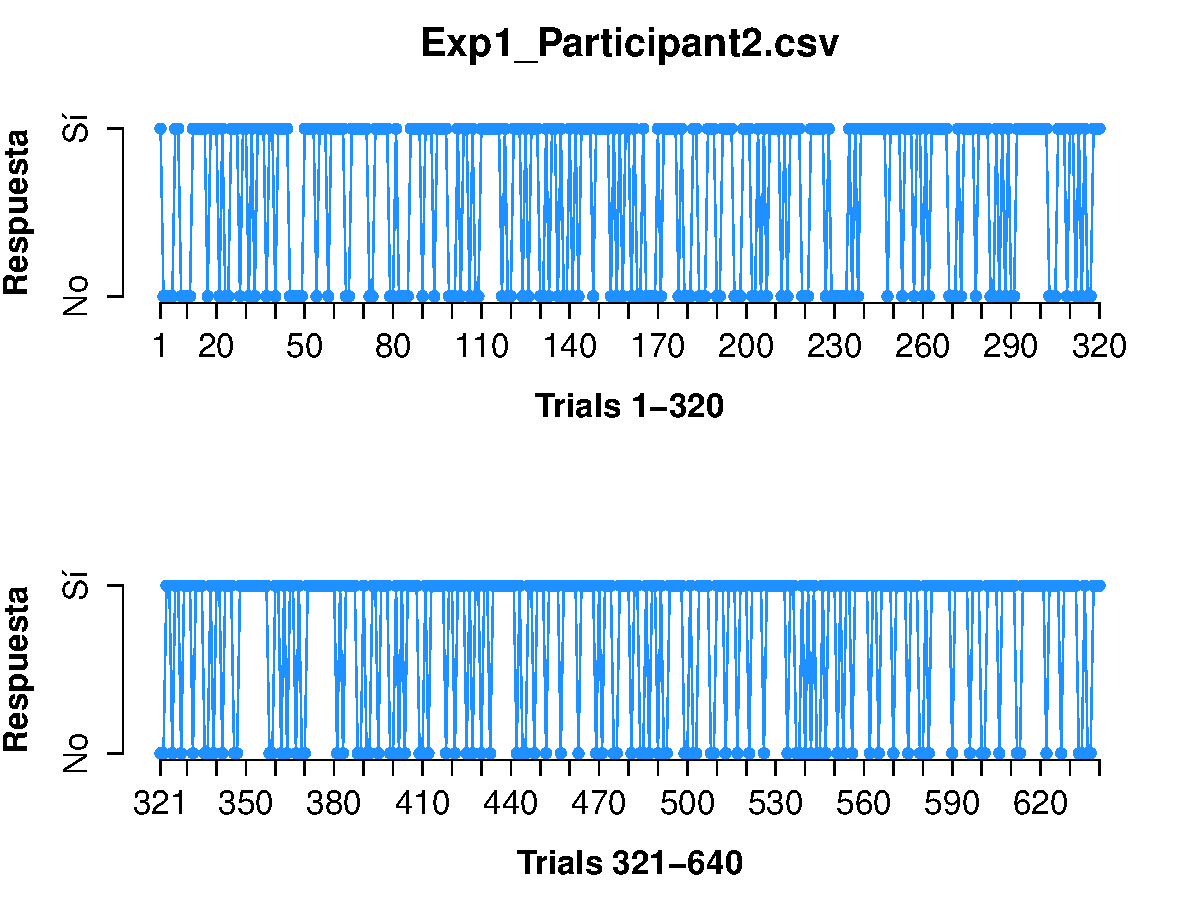
\includegraphics[width=0.30\textwidth]{Figures/Response_Exp1_P2} 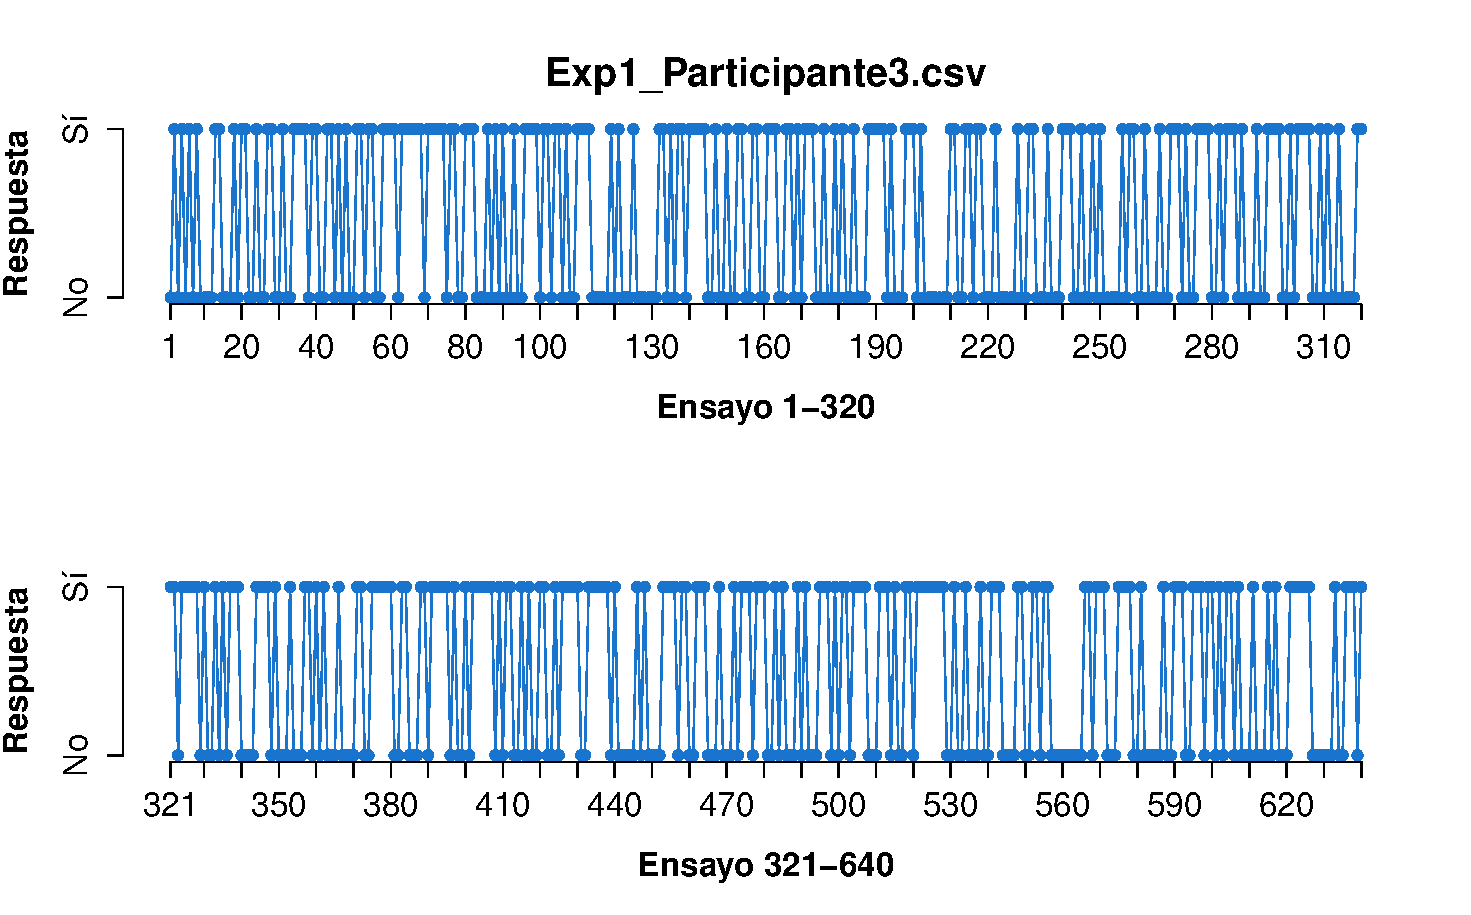
\includegraphics[width=0.30\textwidth]{Figures/Response_Exp1_P3}
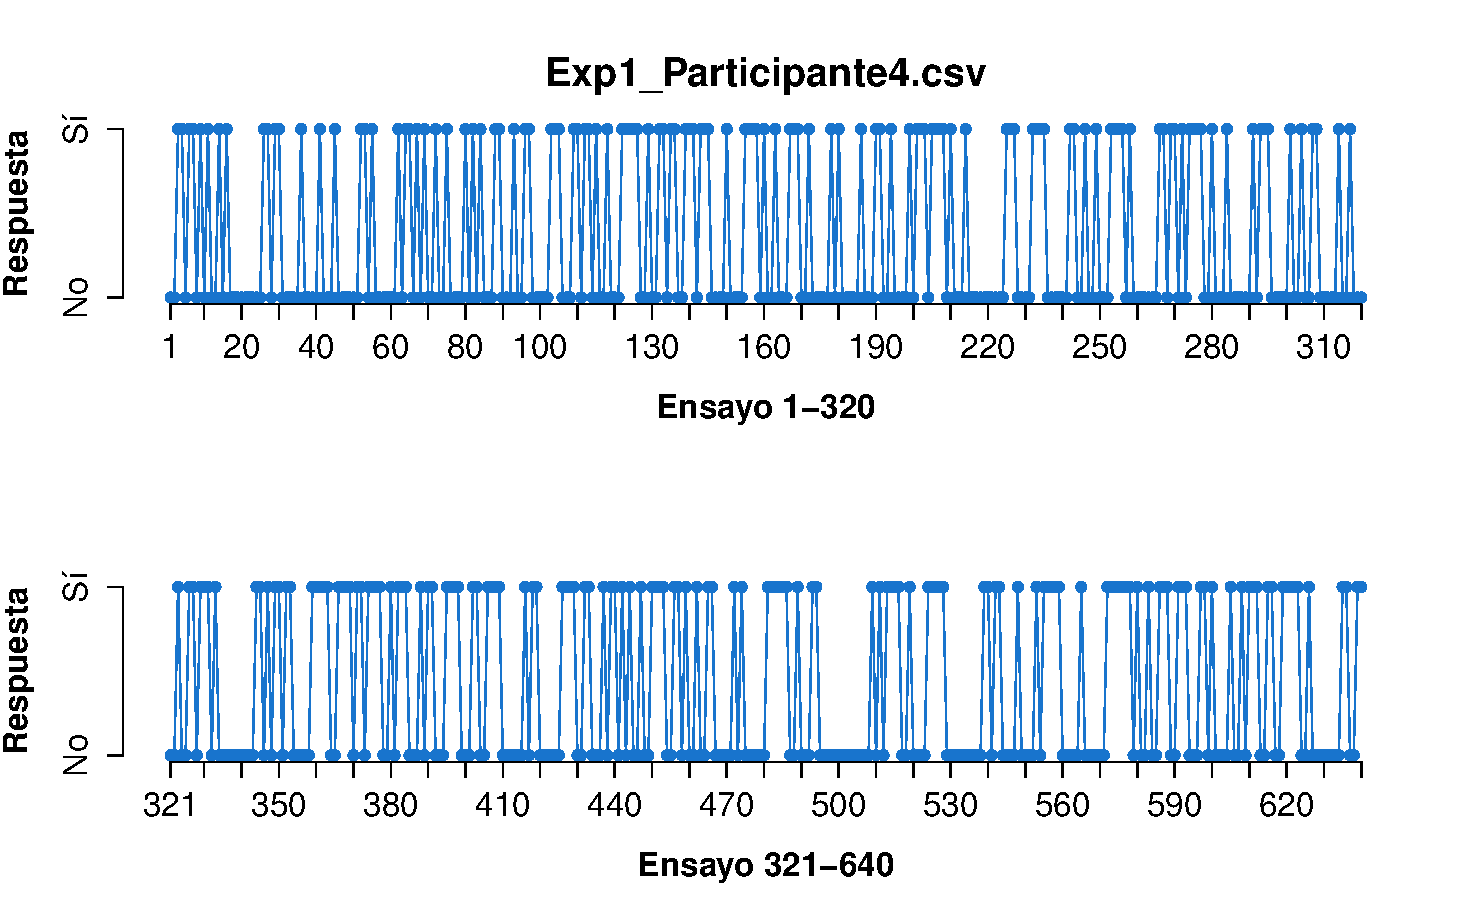
\includegraphics[width=0.30\textwidth]{Figures/Response_Exp1_P4} 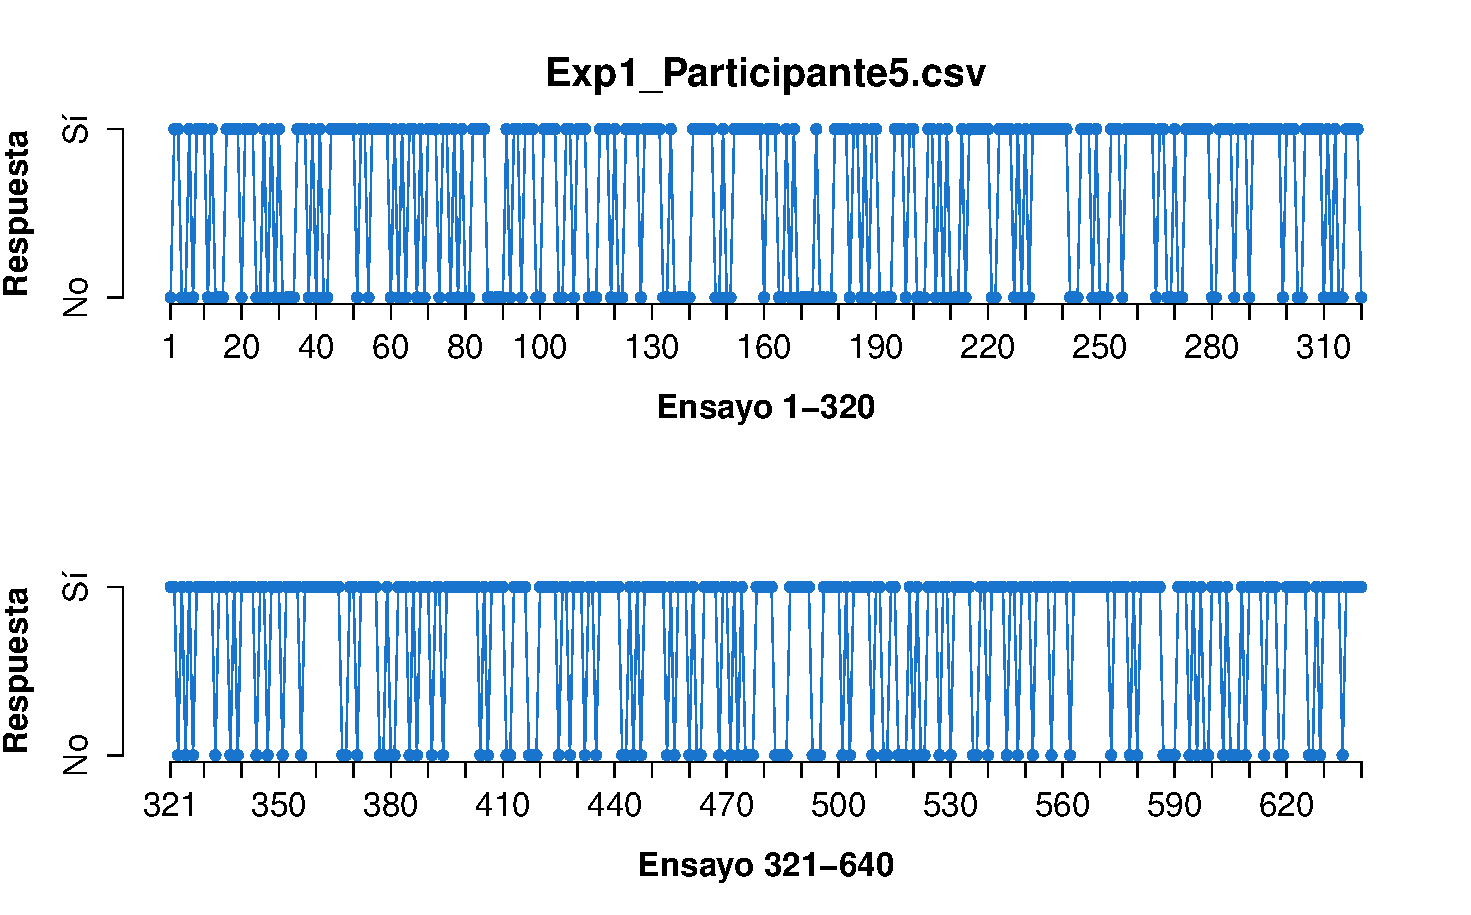
\includegraphics[width=0.30\textwidth]{Figures/Response_Exp1_P5} 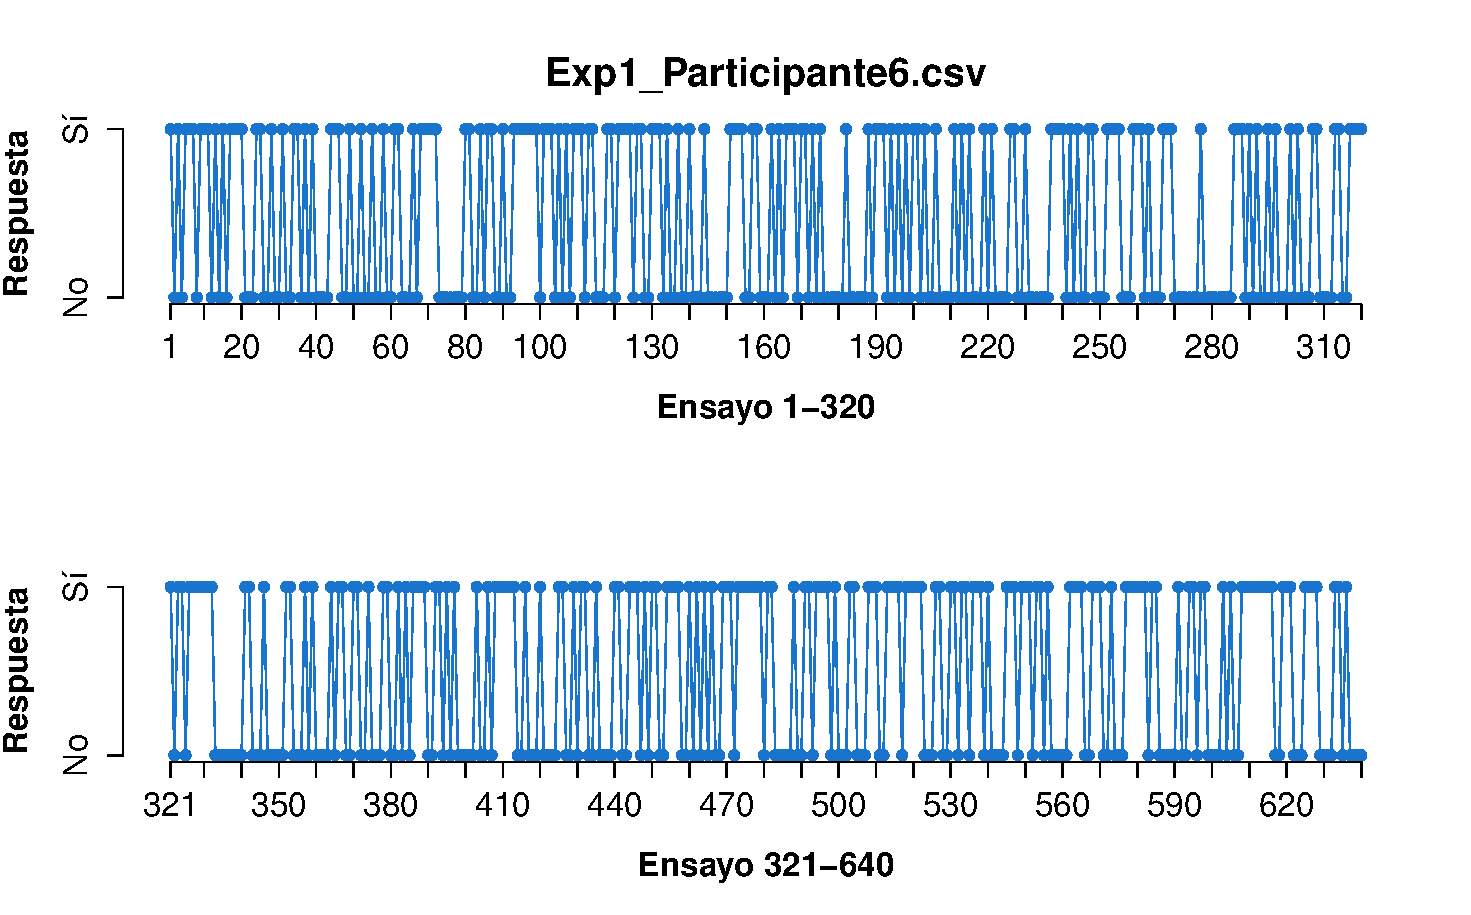
\includegraphics[width=0.30\textwidth]{Figures/Response_Exp1_P6}
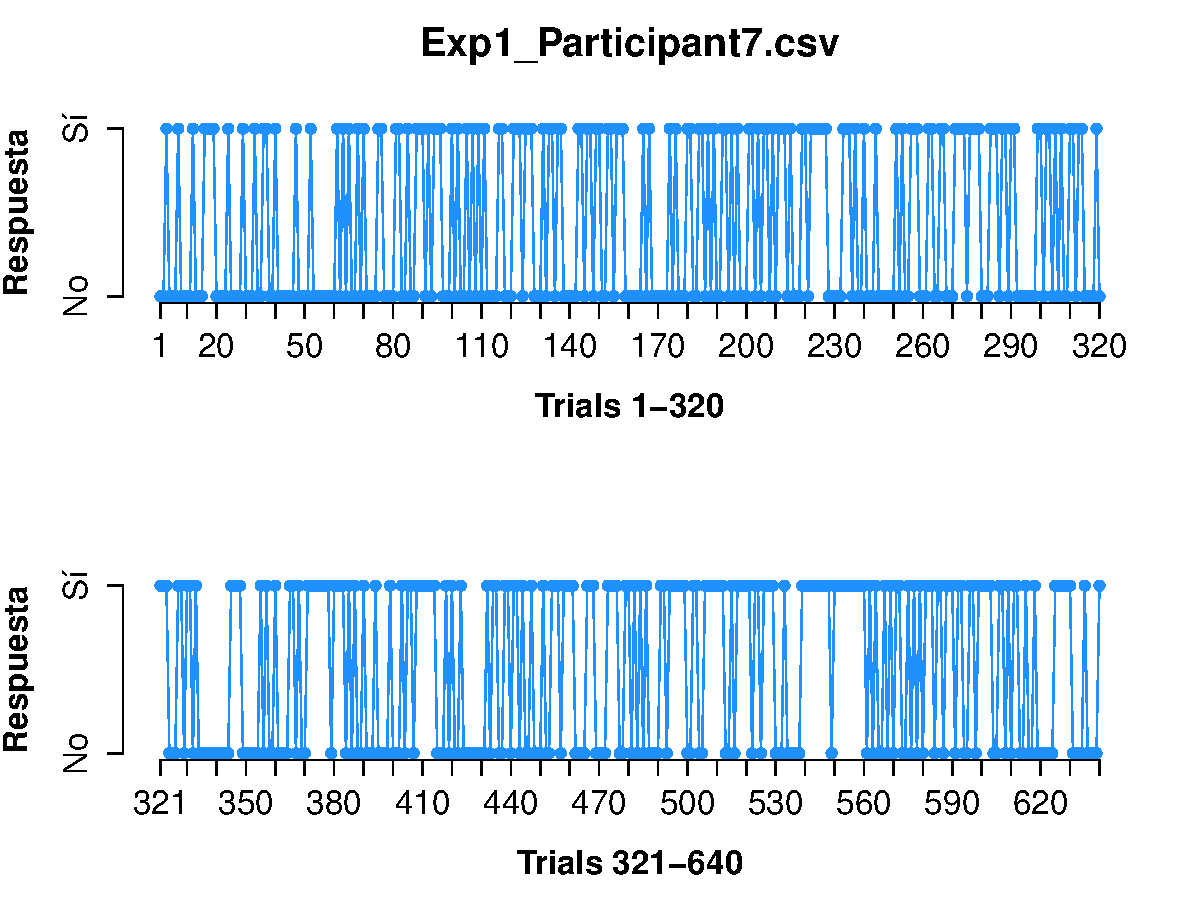
\includegraphics[width=0.30\textwidth]{Figures/Response_Exp1_P7} 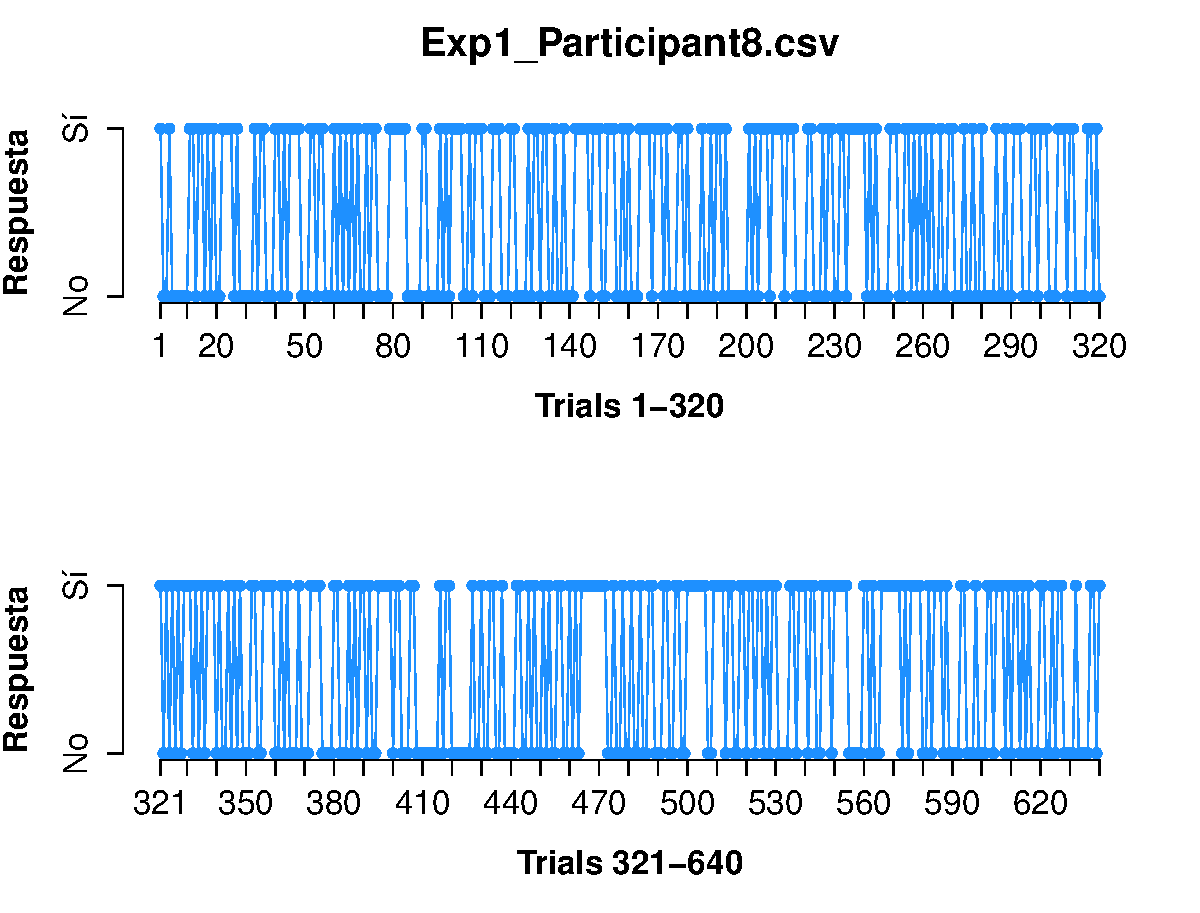
\includegraphics[width=0.30\textwidth]{Figures/Response_Exp1_P8} 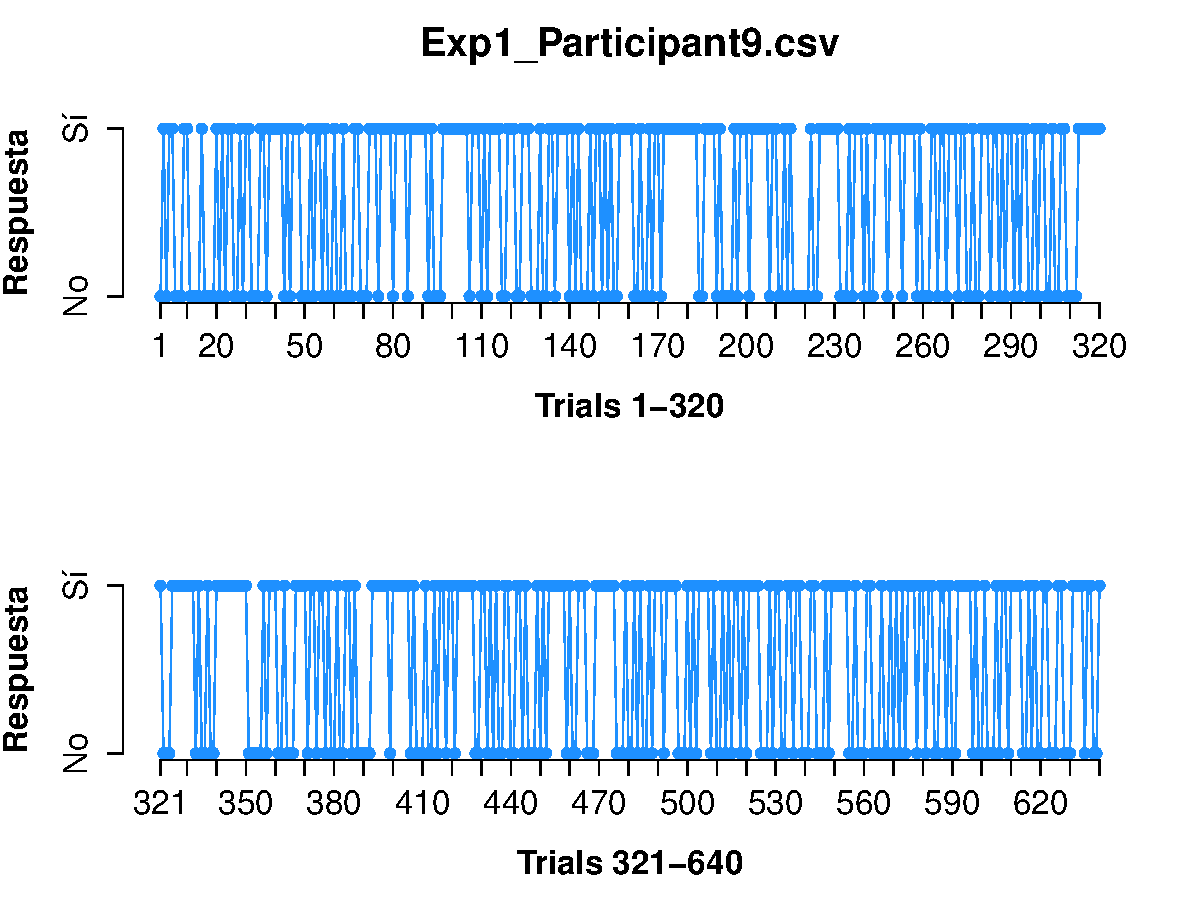
\includegraphics[width=0.30\textwidth]{Figures/Response_Exp1_P9}
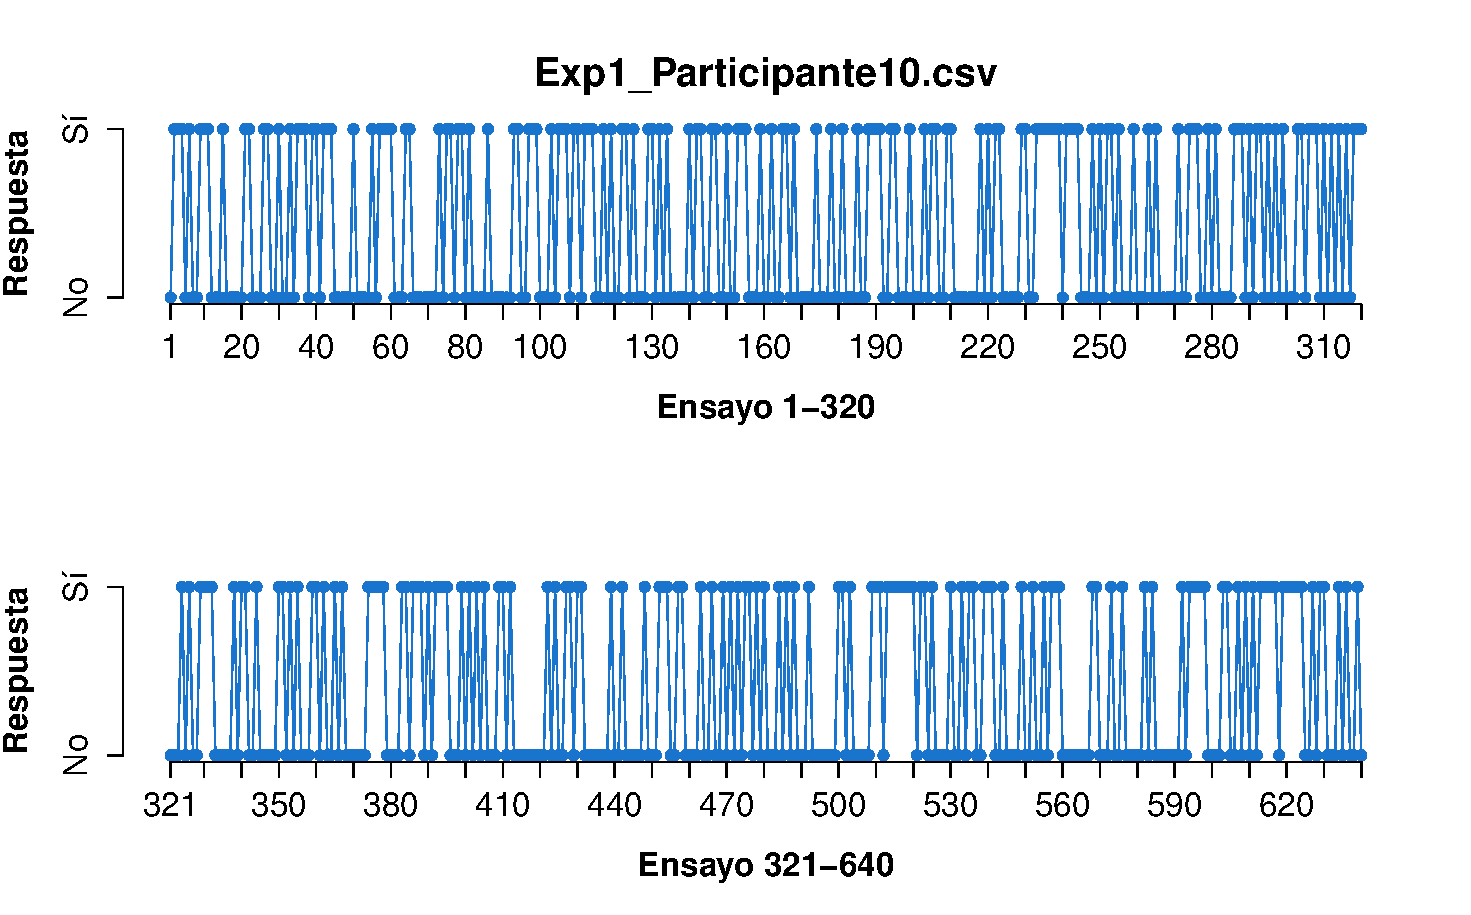
\includegraphics[width=0.30\textwidth]{Figures/Response_Exp1_P10} 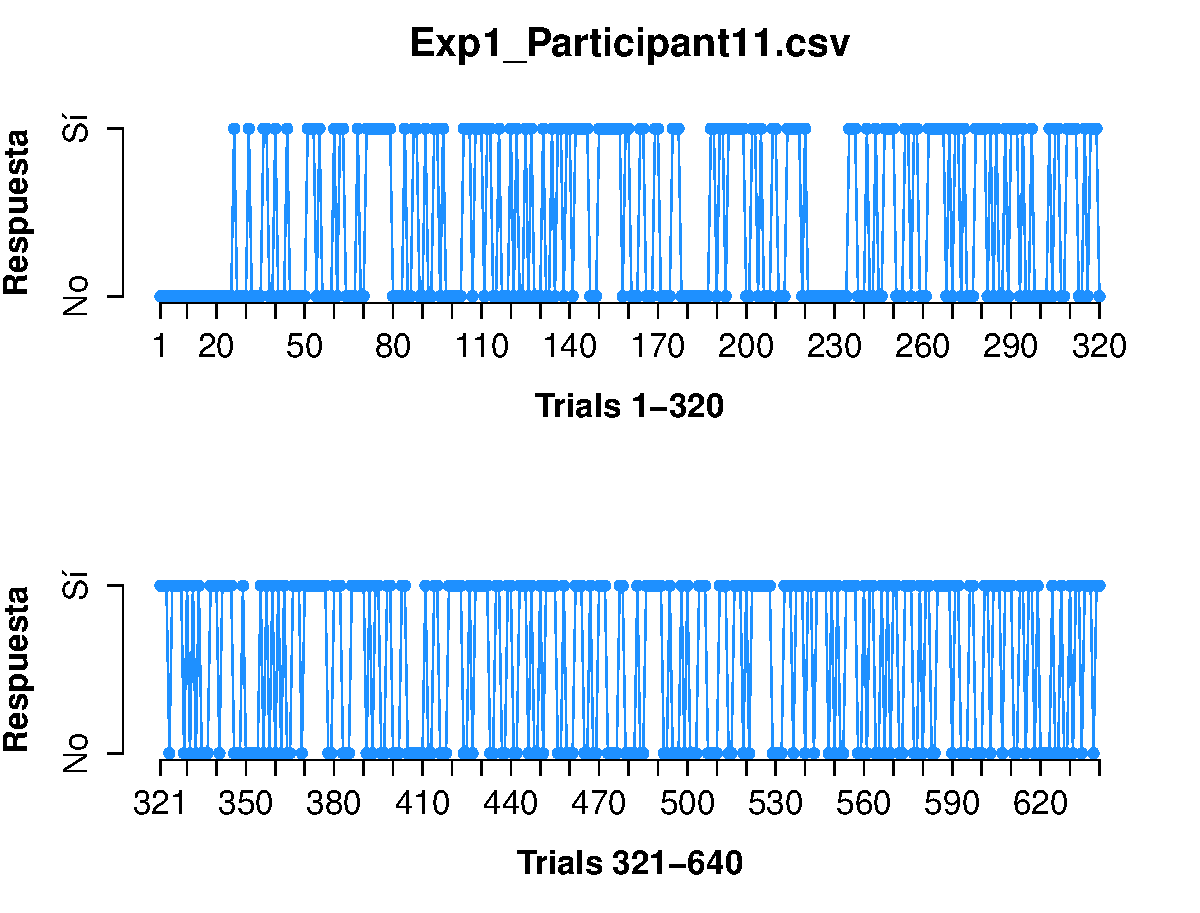
\includegraphics[width=0.30\textwidth]{Figures/Response_Exp1_P11} 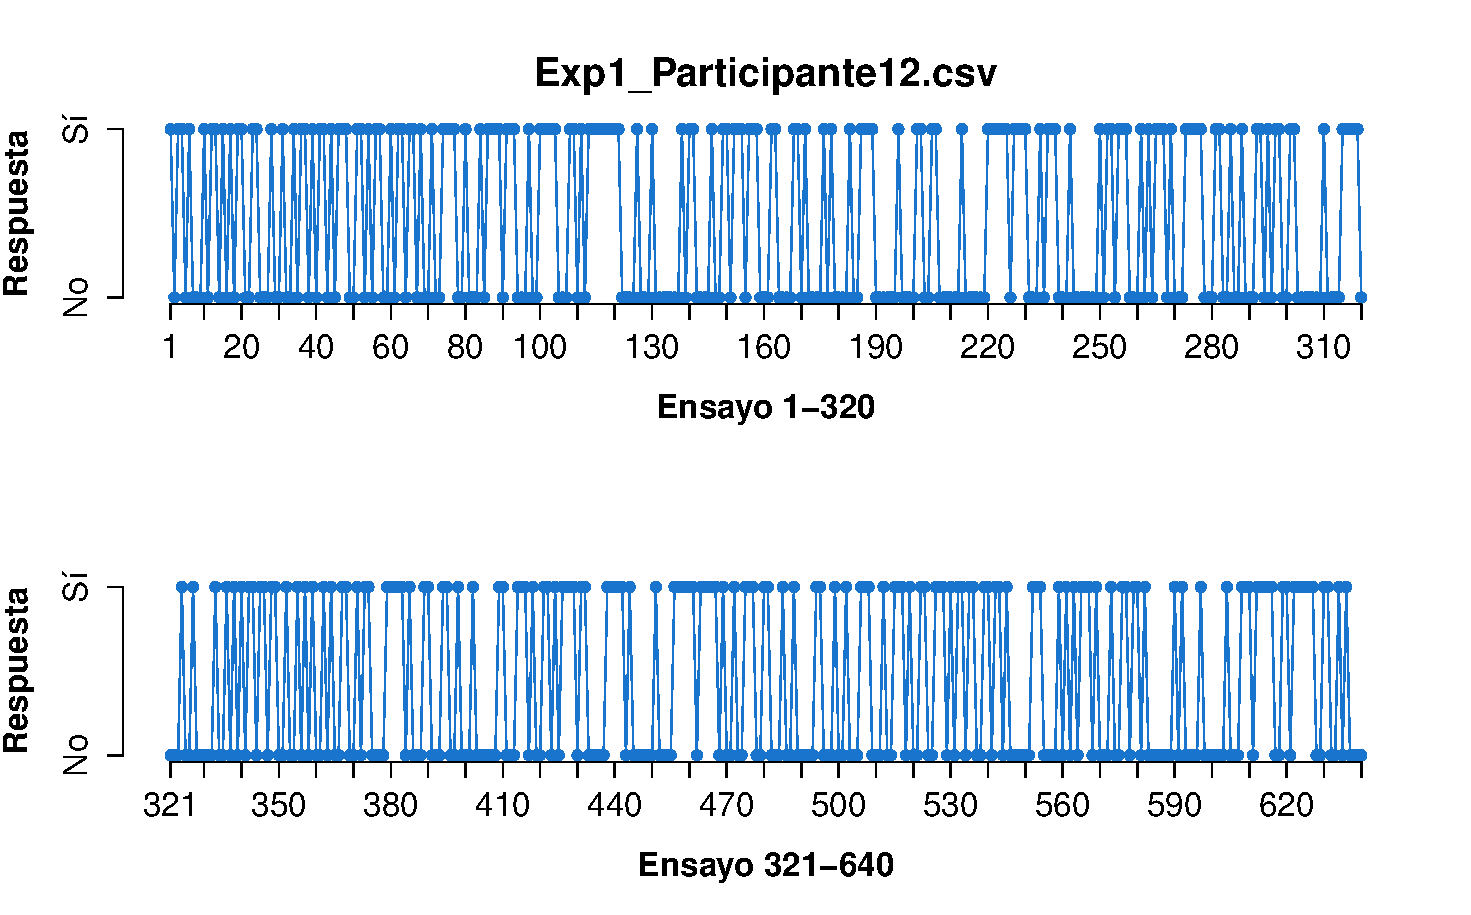
\includegraphics[width=0.30\textwidth]{Figures/Response_Exp1_P12}
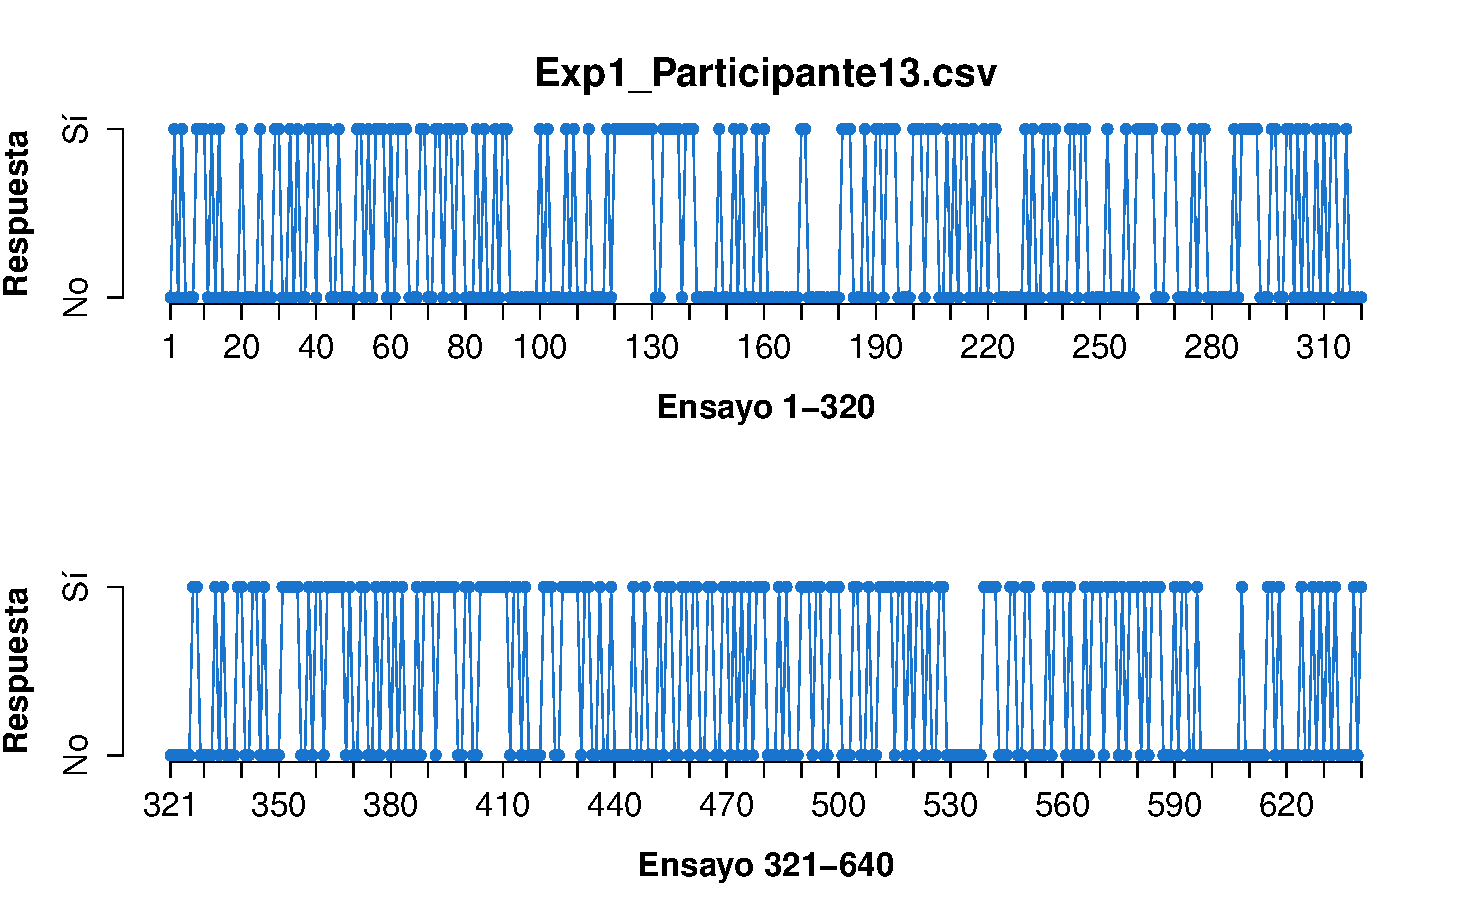
\includegraphics[width=0.30\textwidth]{Figures/Response_Exp1_P13} 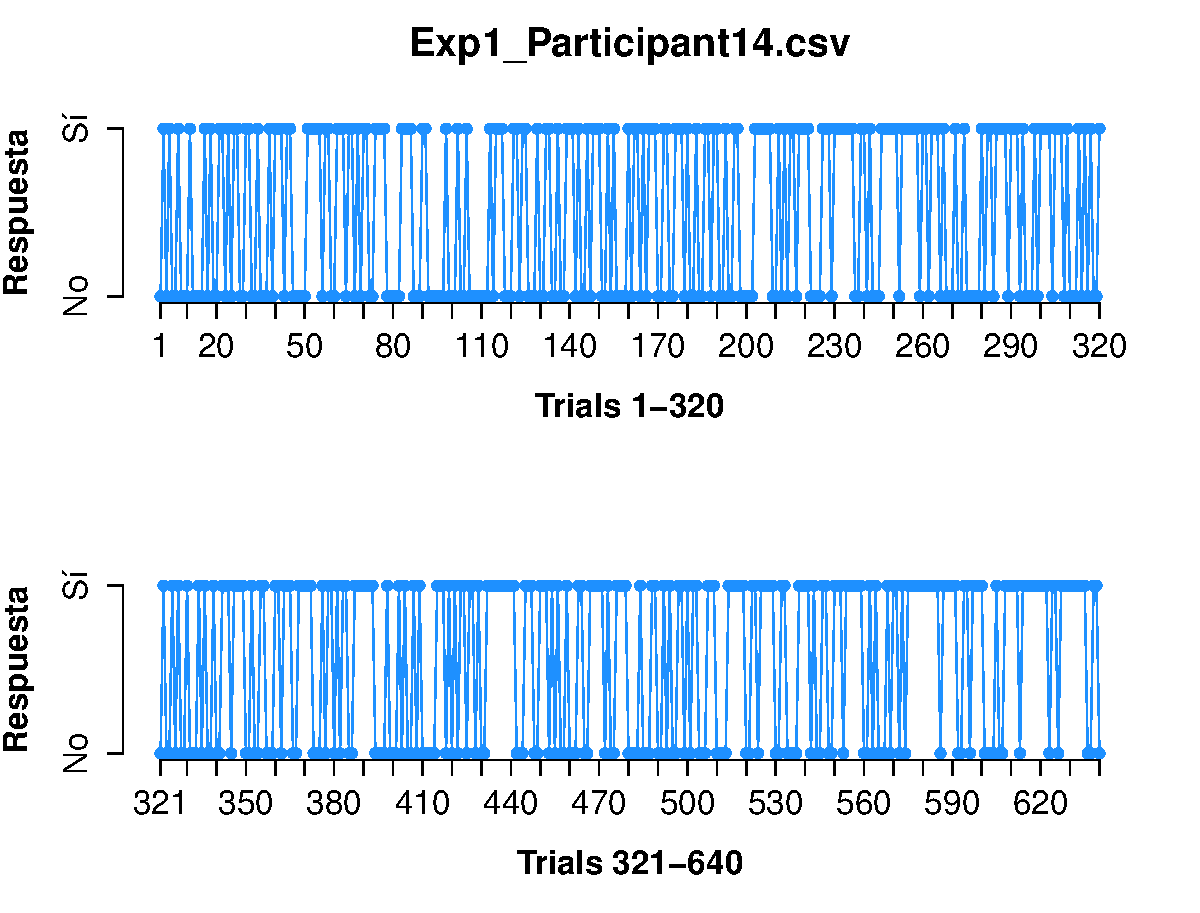
\includegraphics[width=0.30\textwidth]{Figures/Response_Exp1_P14} 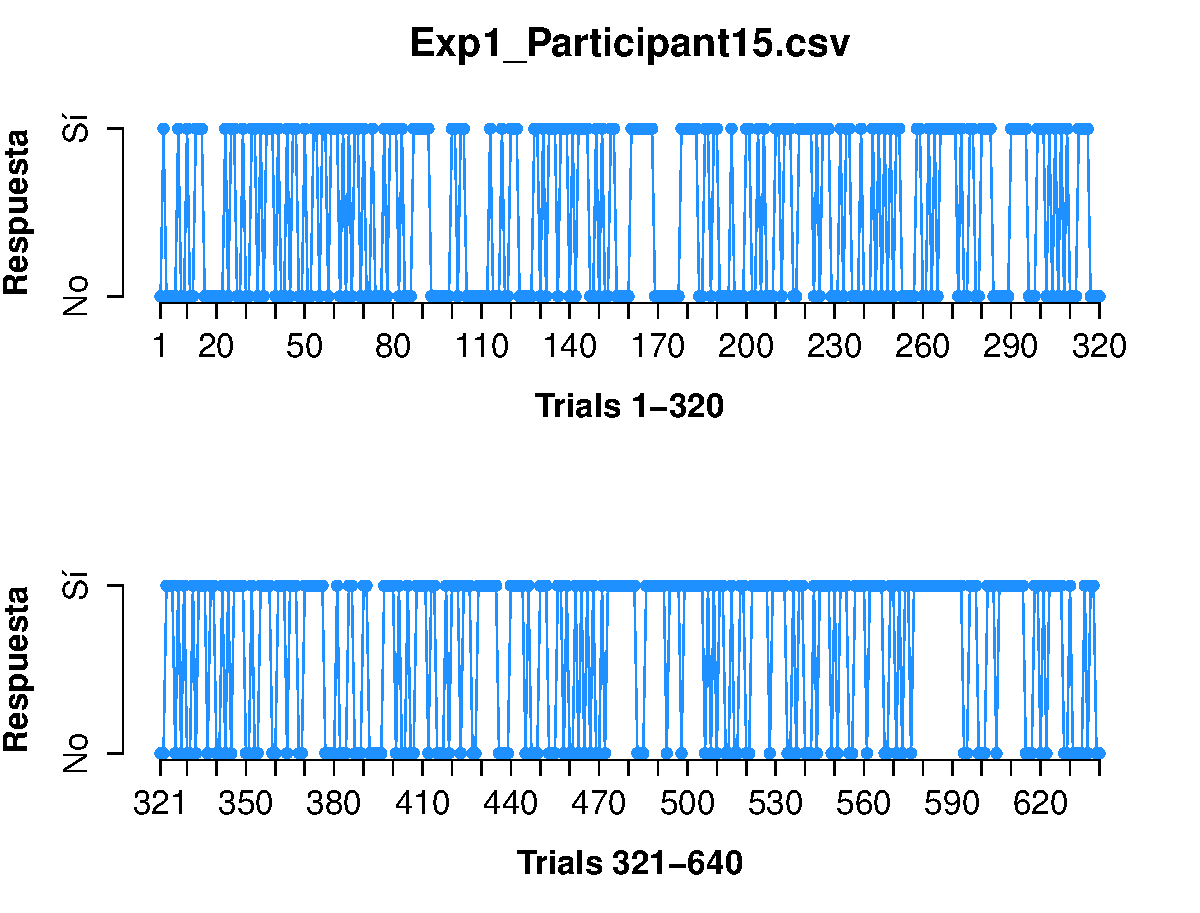
\includegraphics[width=0.30\textwidth]{Figures/Response_Exp1_P15}
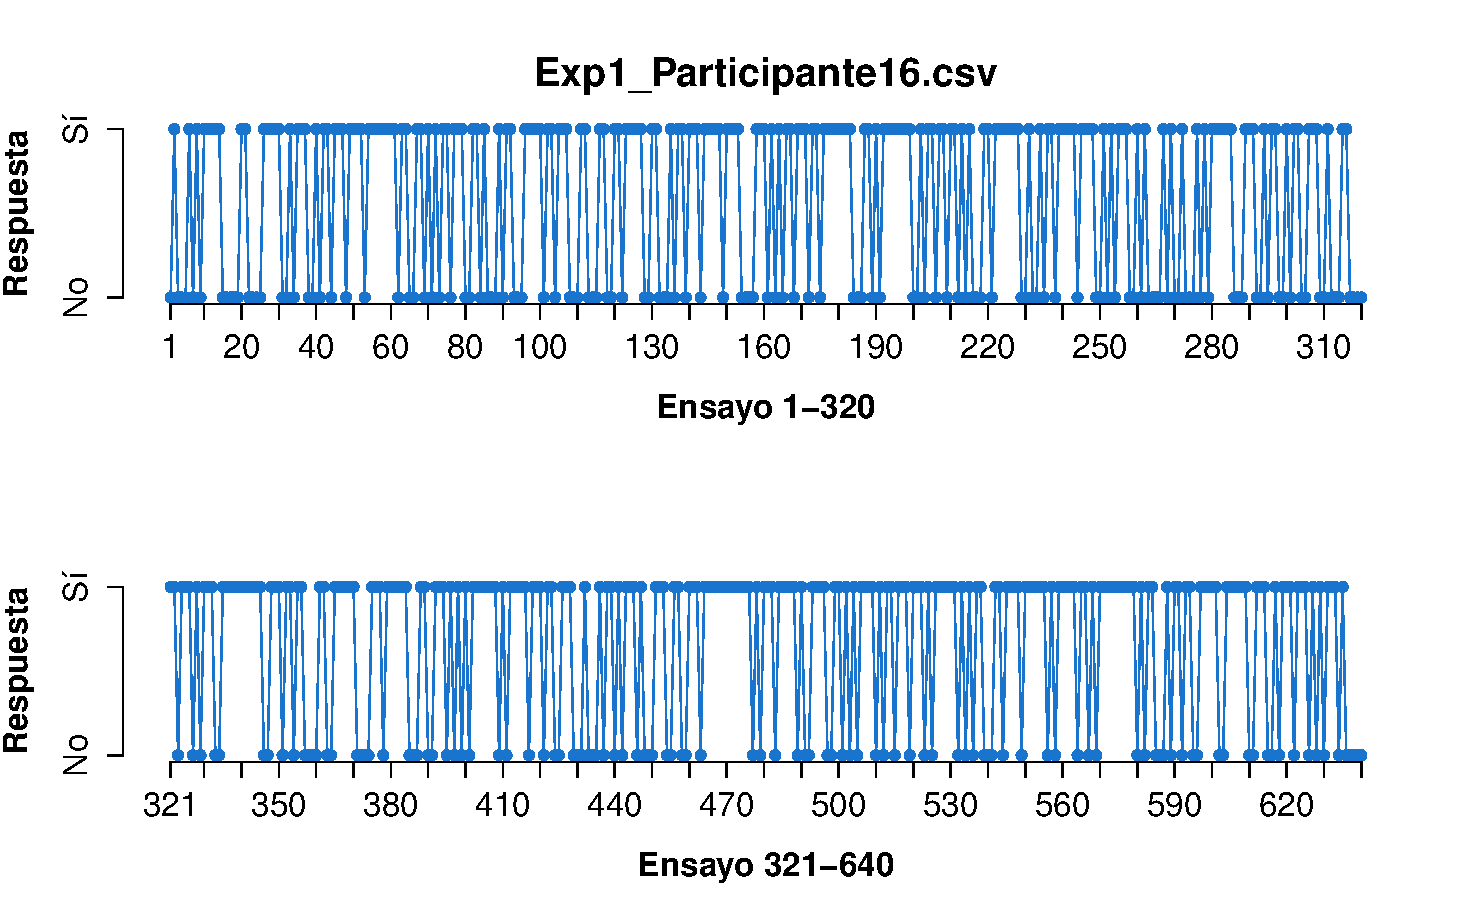
\includegraphics[width=0.30\textwidth]{Figures/Response_Exp1_P16} 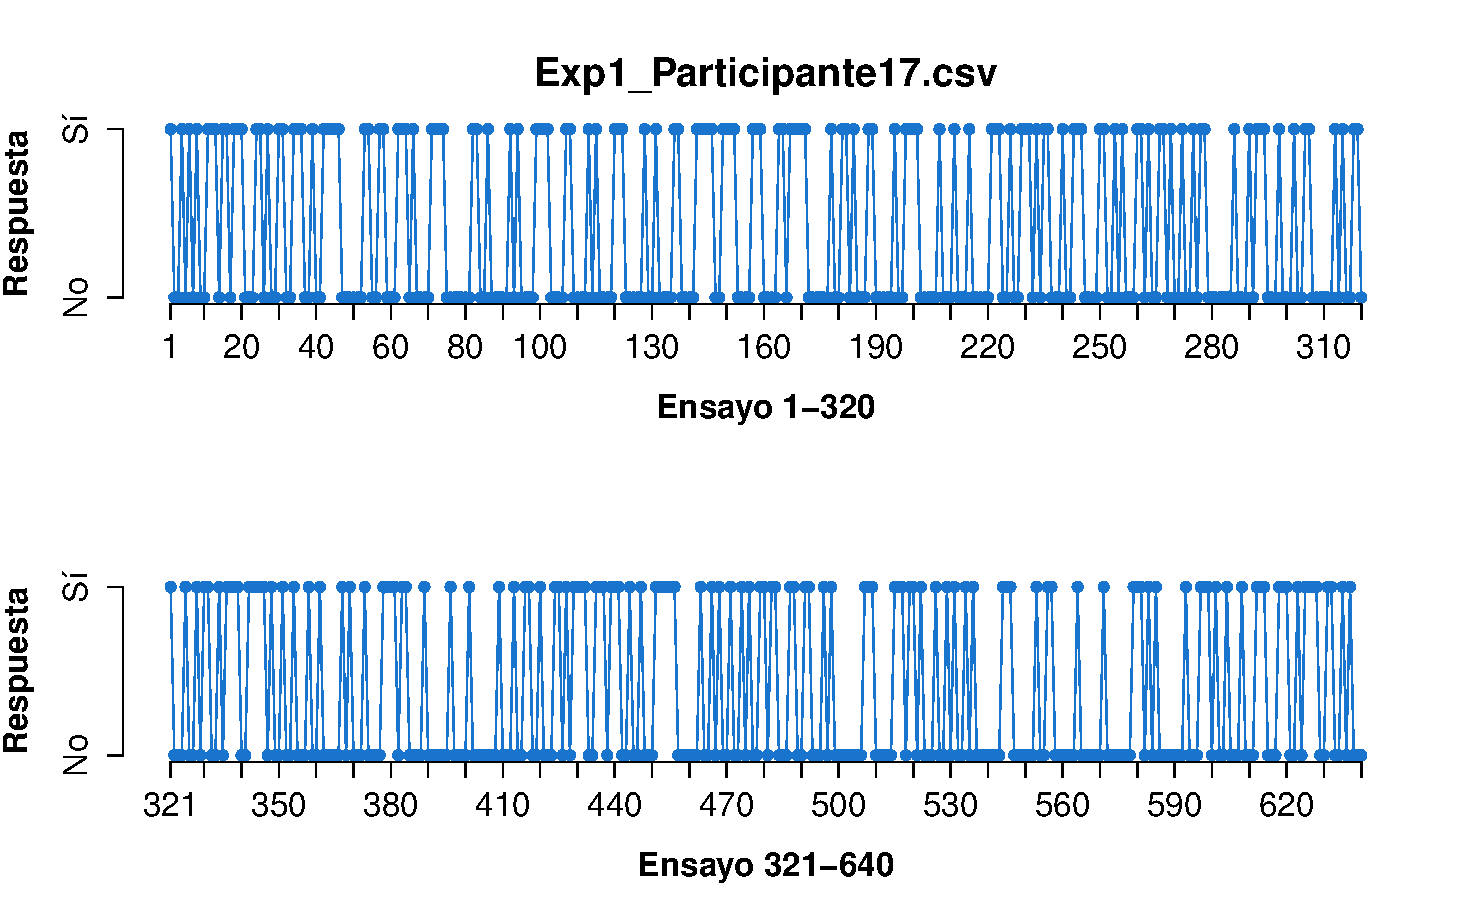
\includegraphics[width=0.30\textwidth]{Figures/Response_Exp1_P17} 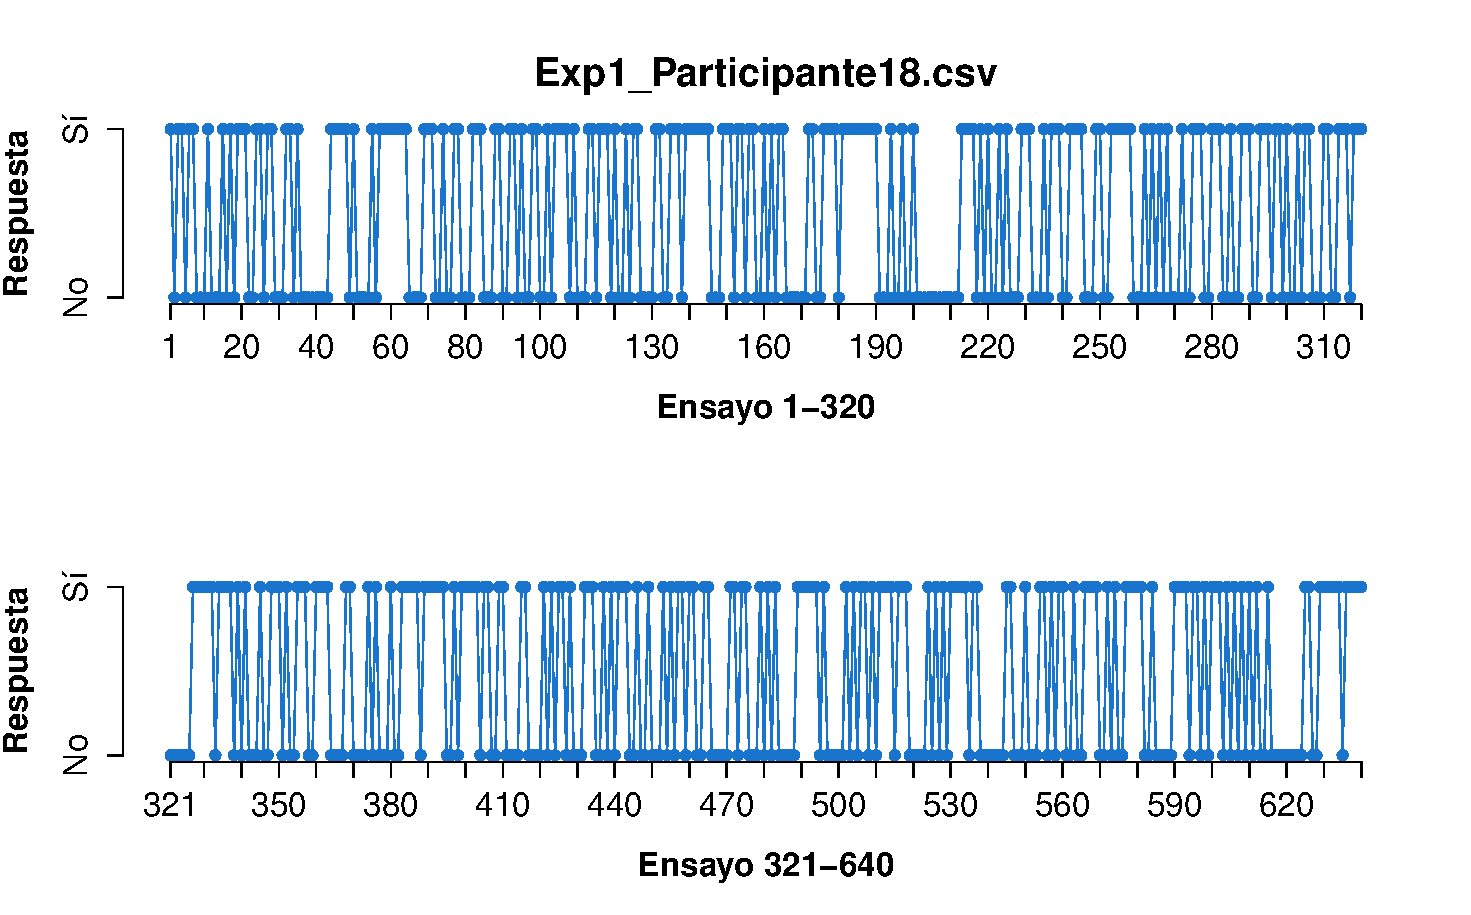
\includegraphics[width=0.30\textwidth]{Figures/Response_Exp1_P18}
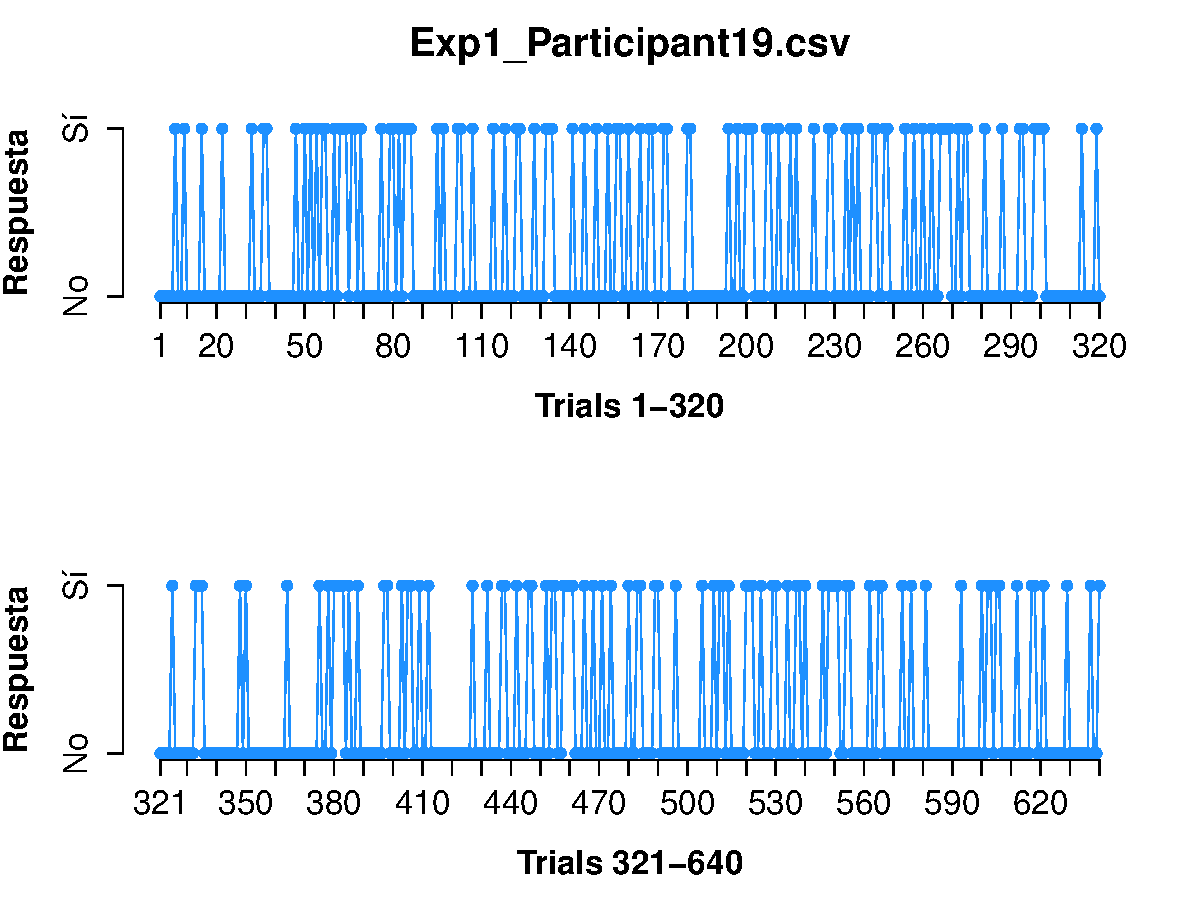
\includegraphics[width=0.30\textwidth]{Figures/Response_Exp1_P19} 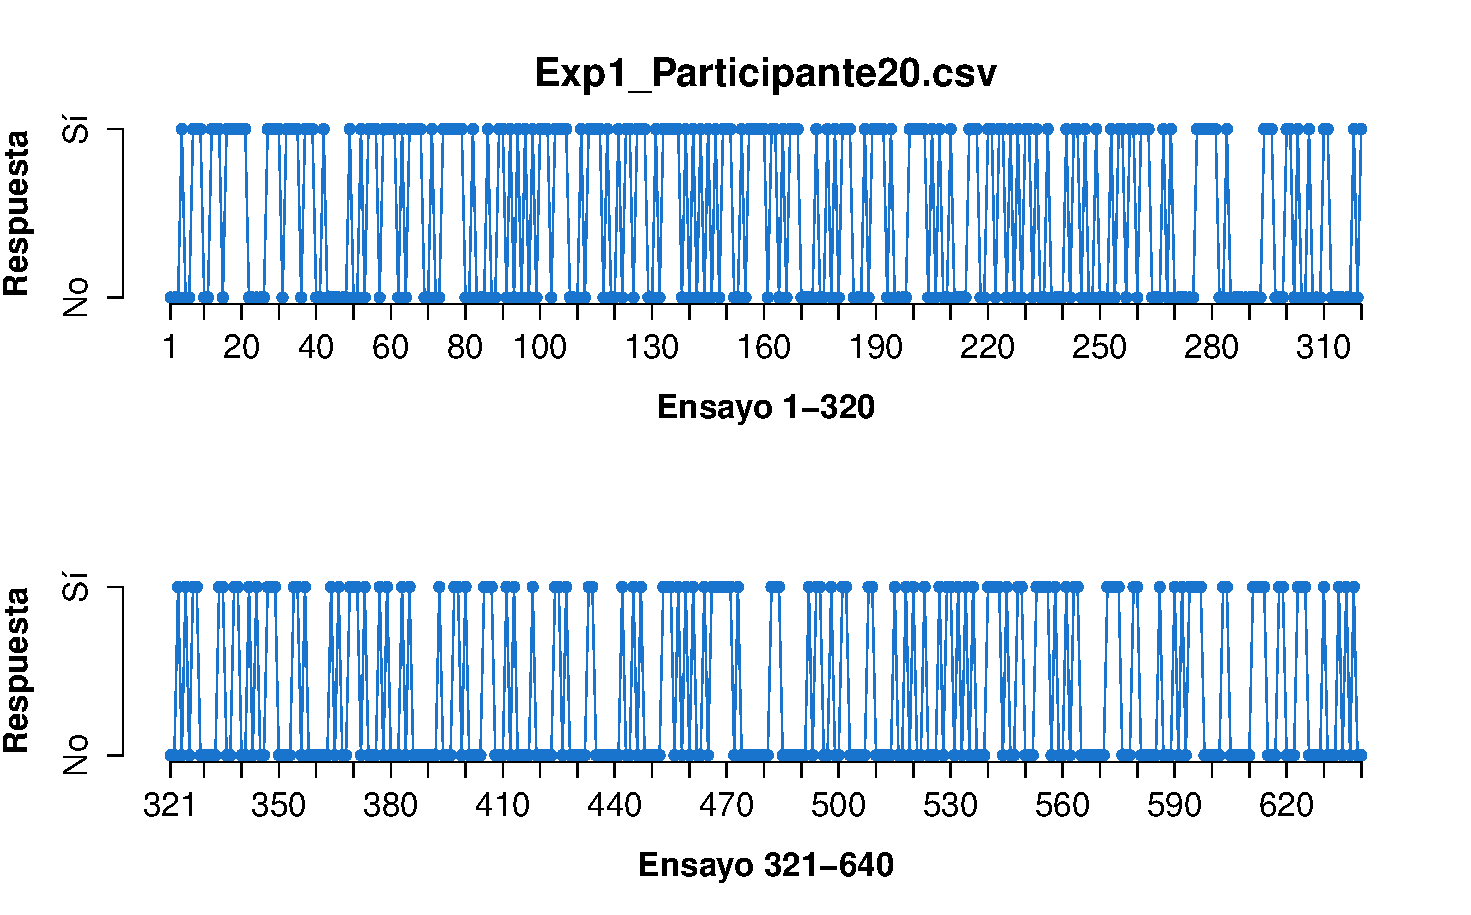
\includegraphics[width=0.30\textwidth]{Figures/Response_Exp1_P20} 
%\decoRule
\caption[Respuesta binaria registrada ensayo a ensayo; Experimento 1]{Respuestas registradas en cada ensayo por los veinte participantes del Experimento 1, para la tarea de detección binaria. Por cada participante se incluyen dos gráficas que presentan las respuestas emitidas en la primera y la segunda mitad del experimento, (panel superior e inferior, respectivamente).}
\label{fig:Response_E1}
\end{figure}

\begin{figure}[th]
\centering
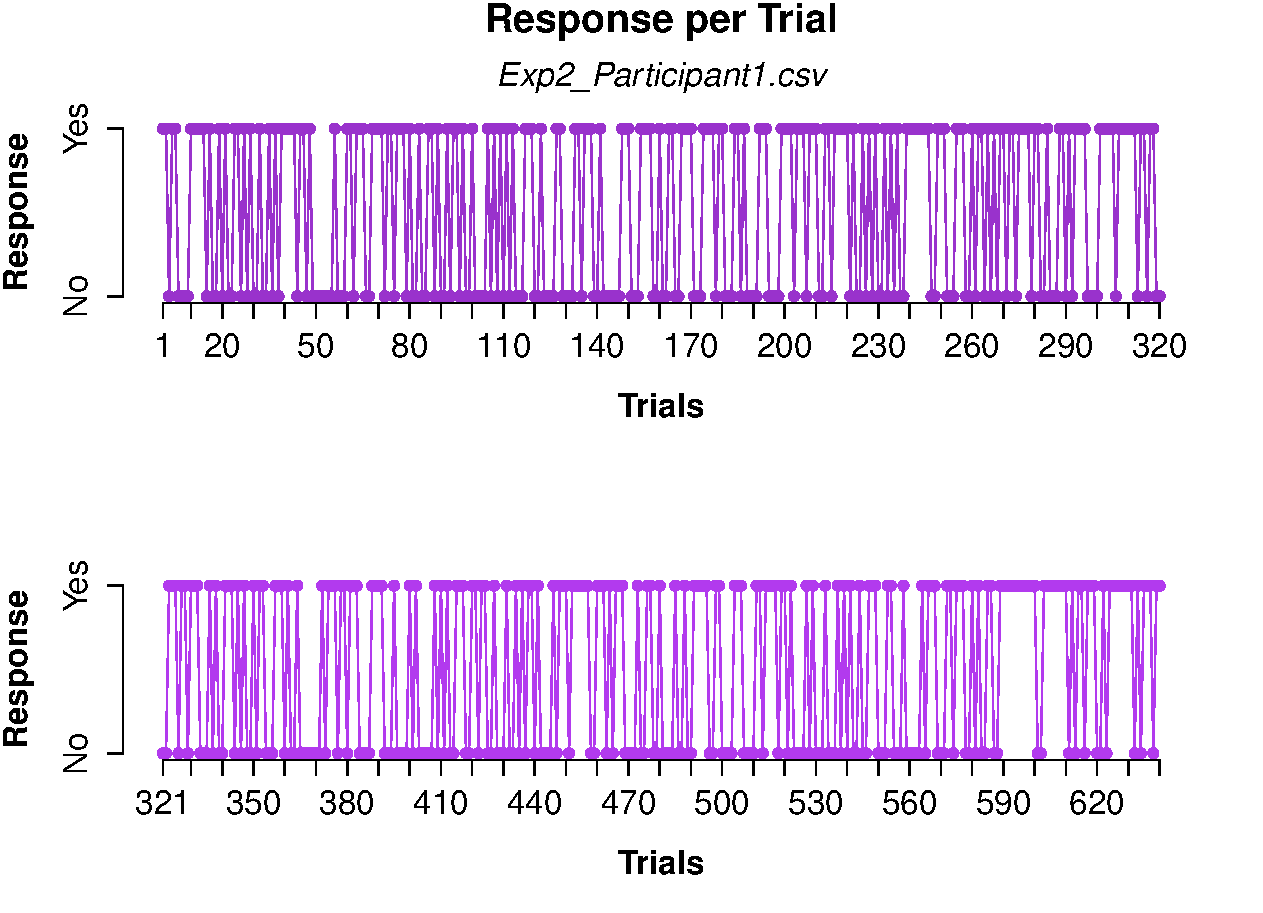
\includegraphics[width=0.30\textwidth]{Figures/Response_Exp2_P1} \includegraphics[width=0.30\textwidth]{Figures/Response_Exp2_P2} \includegraphics[width=0.30\textwidth]{Figures/Response_Exp2_P3}
\includegraphics[width=0.30\textwidth]{Figures/Response_Exp2_P4} \includegraphics[width=0.30\textwidth]{Figures/Response_Exp2_P5} \includegraphics[width=0.30\textwidth]{Figures/Response_Exp2_P6}
\includegraphics[width=0.30\textwidth]{Figures/Response_Exp2_P7} \includegraphics[width=0.30\textwidth]{Figures/Response_Exp2_P8} \includegraphics[width=0.30\textwidth]{Figures/Response_Exp2_P9}
\includegraphics[width=0.30\textwidth]{Figures/Response_Exp2_P10} \includegraphics[width=0.30\textwidth]{Figures/Response_Exp2_P11} \includegraphics[width=0.30\textwidth]{Figures/Response_Exp2_P12}
\includegraphics[width=0.30\textwidth]{Figures/Response_Exp2_P13} \includegraphics[width=0.30\textwidth]{Figures/Response_Exp2_P14} \includegraphics[width=0.30\textwidth]{Figures/Response_Exp2_P15}
\includegraphics[width=0.30\textwidth]{Figures/Response_Exp2_P16} \includegraphics[width=0.30\textwidth]{Figures/Response_Exp2_P17} \includegraphics[width=0.30\textwidth]{Figures/Response_Exp2_P18}
\includegraphics[width=0.30\textwidth]{Figures/Response_Exp2_P19} \includegraphics[width=0.30\textwidth]{Figures/Response_Exp2_P20} \includegraphics[width=0.30\textwidth]{Figures/Response_Exp2_P21} 
%\decoRule
\caption[Respuesta binaria registrada ensayo a ensayo; Experimento 2]{Respuestas registradas por ensayo en la tarea de detección binaria por cada uno de los veintiun participantes del Experimento 2. Las elecciones por participante se muestran en dos páneles que corresponden a los primeros y los últimos 320 ensayos del experimento (panel superior e inferior, respectivamente).}
\label{fig:Response_E2}
\end{figure}

\begin{figure}[th]
\centering
\includegraphics[width=0.30\textwidth]{Figures/BiasResp_Exp1_P1} \includegraphics[width=0.30\textwidth]{Figures/BiasResp_Exp1_P2} \includegraphics[width=0.30\textwidth]{Figures/BiasResp_Exp1_P3}
\includegraphics[width=0.30\textwidth]{Figures/BiasResp_Exp1_P4} \includegraphics[width=0.30\textwidth]{Figures/BiasResp_Exp1_P5} \includegraphics[width=0.30\textwidth]{Figures/BiasResp_Exp1_P6}
\includegraphics[width=0.30\textwidth]{Figures/BiasResp_Exp1_P7} \includegraphics[width=0.30\textwidth]{Figures/BiasResp_Exp1_P8} \includegraphics[width=0.30\textwidth]{Figures/BiasResp_Exp1_P9}
\includegraphics[width=0.30\textwidth]{Figures/BiasResp_Exp1_P10} \includegraphics[width=0.30\textwidth]{Figures/BiasResp_Exp1_P11} \includegraphics[width=0.30\textwidth]{Figures/BiasResp_Exp1_P12}
\includegraphics[width=0.30\textwidth]{Figures/BiasResp_Exp1_P13} \includegraphics[width=0.30\textwidth]{Figures/BiasResp_Exp1_P14} \includegraphics[width=0.30\textwidth]{Figures/BiasResp_Exp1_P15}
\includegraphics[width=0.30\textwidth]{Figures/BiasResp_Exp1_P16} \includegraphics[width=0.30\textwidth]{Figures/BiasResp_Exp1_P17} \includegraphics[width=0.30\textwidth]{Figures/BiasResp_Exp1_P18}
\includegraphics[width=0.30\textwidth]{Figures/BiasResp_Exp1_P19} \includegraphics[width=0.30\textwidth]{Figures/BiasResp_Exp1_P20} 
%\decoRule
\caption[Respuesta binaria registrada ensayo a ensayo en relación con el tipo de estímulo a evaluar; Experimento 1]{Respuesta registrada en cada ensayo para la tarea de detección binaria, por los veinte participantes del Experimento 1. Por cada participante se muestran dos gráficas que señalan con colores diferentes el tipo de estímulo presente en cada ensayo: En la parte superior, se señala si los estímulos eran de la condición fácil o difícil (con colores azul y violeta, respectivamente) y en la parte inferior, se distinguen los ensayos con señal y ruido presentándolos en color verde y rojo, respectivamente.}
\label{fig:BiasResp_E1}
\end{figure}

\begin{figure}[th]
\centering
\includegraphics[width=0.30\textwidth]{Figures/BiasResp_Exp2_P1} \includegraphics[width=0.30\textwidth]{Figures/BiasResp_Exp2_P2} \includegraphics[width=0.30\textwidth]{Figures/BiasResp_Exp2_P3}
\includegraphics[width=0.30\textwidth]{Figures/BiasResp_Exp2_P4} \includegraphics[width=0.30\textwidth]{Figures/BiasResp_Exp2_P5} \includegraphics[width=0.30\textwidth]{Figures/BiasResp_Exp2_P6}
\includegraphics[width=0.30\textwidth]{Figures/BiasResp_Exp2_P7} \includegraphics[width=0.30\textwidth]{Figures/BiasResp_Exp2_P8} \includegraphics[width=0.30\textwidth]{Figures/BiasResp_Exp2_P9}
\includegraphics[width=0.30\textwidth]{Figures/BiasResp_Exp2_P10} \includegraphics[width=0.30\textwidth]{Figures/BiasResp_Exp2_P11} \includegraphics[width=0.30\textwidth]{Figures/BiasResp_Exp2_P12}
\includegraphics[width=0.30\textwidth]{Figures/BiasResp_Exp2_P13} \includegraphics[width=0.30\textwidth]{Figures/BiasResp_Exp2_P14} \includegraphics[width=0.30\textwidth]{Figures/BiasResp_Exp2_P15}
\includegraphics[width=0.30\textwidth]{Figures/BiasResp_Exp2_P16} \includegraphics[width=0.30\textwidth]{Figures/BiasResp_Exp2_P17} \includegraphics[width=0.30\textwidth]{Figures/BiasResp_Exp2_P18}
\includegraphics[width=0.30\textwidth]{Figures/BiasResp_Exp2_P19} \includegraphics[width=0.30\textwidth]{Figures/BiasResp_Exp2_P20} \includegraphics[width=0.30\textwidth]{Figures/BiasResp_Exp2_P21}
%\decoRule
\caption[Respuesta binaria registrada ensayo a ensayo en relación con el tipo de estímulo a evaluar; Experimento 2]{Respuesta registrada por ensayo en la tarea de detección binaria por los veintiun participantes del Experimento 2. Por cada participante se muestran dos gráficas que señalan con colores diferentes el tipo de estímulo evaluado en cada ensayo: En la parte superior, se señala la condición de dificultad (azul para fácil y violeta para difícil) y en la parte inferior, el tipo de ensayo (las señales en verde y en rojo los ensayos con ruido).}
\label{fig:BiasResp_E2}
\end{figure}

\begin{figure}[th]
\centering
\includegraphics[width=0.30\textwidth]{Figures/Rating_Exp1_P1} \includegraphics[width=0.30\textwidth]{Figures/Rating_Exp1_P2} \includegraphics[width=0.30\textwidth]{Figures/Rating_Exp1_P3}
\includegraphics[width=0.30\textwidth]{Figures/Rating_Exp1_P4} \includegraphics[width=0.30\textwidth]{Figures/Rating_Exp1_P5} \includegraphics[width=0.30\textwidth]{Figures/Rating_Exp1_P6}
\includegraphics[width=0.30\textwidth]{Figures/Rating_Exp1_P7} \includegraphics[width=0.30\textwidth]{Figures/Rating_Exp1_P8} \includegraphics[width=0.30\textwidth]{Figures/Rating_Exp1_P9}
\includegraphics[width=0.30\textwidth]{Figures/Rating_Exp1_P10} \includegraphics[width=0.30\textwidth]{Figures/Rating_Exp1_P11} \includegraphics[width=0.30\textwidth]{Figures/Rating_Exp1_P12}
\includegraphics[width=0.30\textwidth]{Figures/Rating_Exp1_P13} \includegraphics[width=0.30\textwidth]{Figures/Rating_Exp1_P14} \includegraphics[width=0.30\textwidth]{Figures/Rating_Exp1_P15}
\includegraphics[width=0.30\textwidth]{Figures/Rating_Exp1_P16} \includegraphics[width=0.30\textwidth]{Figures/Rating_Exp1_P17} \includegraphics[width=0.30\textwidth]{Figures/Rating_Exp1_P18}
\includegraphics[width=0.30\textwidth]{Figures/Rating_Exp1_P19} \includegraphics[width=0.30\textwidth]{Figures/Rating_Exp1_P20} 
%\decoRule
\caption[Puntajes de Confianza asignados ensayo a ensayo; Experimento 1]{Puntaje de confianza asignado a las respuestas binarias emitidas ensayo a ensayo por cada participante del Experimento 1. Se despliegan las elecciones de cada participante un panel superior e inferior, que presentan los primeros y los últimos 320 ensayos del experimento, respectivamente.}
\label{fig:Rating_E1}
\end{figure}

\begin{figure}[th]
\centering
\includegraphics[width=0.30\textwidth]{Figures/Rating_Exp2_P1} \includegraphics[width=0.30\textwidth]{Figures/Rating_Exp2_P2} \includegraphics[width=0.30\textwidth]{Figures/Rating_Exp2_P3}
\includegraphics[width=0.30\textwidth]{Figures/Rating_Exp2_P4} \includegraphics[width=0.30\textwidth]{Figures/Rating_Exp2_P5} \includegraphics[width=0.30\textwidth]{Figures/Rating_Exp2_P6}
\includegraphics[width=0.30\textwidth]{Figures/Rating_Exp2_P7} \includegraphics[width=0.30\textwidth]{Figures/Rating_Exp2_P8} \includegraphics[width=0.30\textwidth]{Figures/Rating_Exp2_P9}
\includegraphics[width=0.30\textwidth]{Figures/Rating_Exp2_P10} \includegraphics[width=0.30\textwidth]{Figures/Rating_Exp2_P11} \includegraphics[width=0.30\textwidth]{Figures/Rating_Exp2_P12}
\includegraphics[width=0.30\textwidth]{Figures/Rating_Exp2_P13} \includegraphics[width=0.30\textwidth]{Figures/Rating_Exp2_P14} \includegraphics[width=0.30\textwidth]{Figures/Rating_Exp2_P15}
\includegraphics[width=0.30\textwidth]{Figures/Rating_Exp2_P16} \includegraphics[width=0.30\textwidth]{Figures/Rating_Exp2_P17} \includegraphics[width=0.30\textwidth]{Figures/Rating_Exp2_P18}
\includegraphics[width=0.30\textwidth]{Figures/Rating_Exp2_P19} \includegraphics[width=0.30\textwidth]{Figures/Rating_Exp2_P20} \includegraphics[width=0.30\textwidth]{Figures/Rating_Exp2_P21}
%\decoRule
\caption[Puntajes de Confianza asignados ensayo a ensayo; Experimento 2]{Puntaje de confianza asignado a las respuestas binarias emitidas ensayo a ensayo por cada participante del Experimento 1. Se despliegan las elecciones de cada participante un panel superior e inferior, que presentan los primeros y los últimos 320 ensayos del experimento, respectivamente.}
\label{fig:Rating_E2}
\end{figure}











\begin{figure}[th]
\centering
\includegraphics[width=0.30\textwidth]{Figures/Success_Exp1_P1} \includegraphics[width=0.30\textwidth]{Figures/Success_Exp1_P2} \includegraphics[width=0.30\textwidth]{Figures/Success_Exp1_P3}
\includegraphics[width=0.30\textwidth]{Figures/Success_Exp1_P4} \includegraphics[width=0.30\textwidth]{Figures/Success_Exp1_P5} \includegraphics[width=0.30\textwidth]{Figures/Success_Exp1_P6}
\includegraphics[width=0.30\textwidth]{Figures/Success_Exp1_P7} \includegraphics[width=0.30\textwidth]{Figures/Success_Exp1_P8} \includegraphics[width=0.30\textwidth]{Figures/Success_Exp1_P9}
\includegraphics[width=0.30\textwidth]{Figures/Success_Exp1_P10} \includegraphics[width=0.30\textwidth]{Figures/Success_Exp1_P11} \includegraphics[width=0.30\textwidth]{Figures/Success_Exp1_P12}
\includegraphics[width=0.30\textwidth]{Figures/Success_Exp1_P13} \includegraphics[width=0.30\textwidth]{Figures/Success_Exp1_P14} \includegraphics[width=0.30\textwidth]{Figures/Success_Exp1_P15}
\includegraphics[width=0.30\textwidth]{Figures/Success_Exp1_P16} \includegraphics[width=0.30\textwidth]{Figures/Success_Exp1_P17} \includegraphics[width=0.30\textwidth]{Figures/Success_Exp1_P18}
\includegraphics[width=0.30\textwidth]{Figures/Success_Exp1_P19} \includegraphics[width=0.30\textwidth]{Figures/Success_Exp1_P20} 
%\decoRule
\caption[Aciertos y Errores a lo largo del tiempo; Experimento 1]{Aciertos y errores cometidos por los veinte participantes del Experimento 1. Por cada participante se muestra el registro acumulativo de los aciertos y errores registrados a lo largo del tiempo (panel superior) y los aciertos o errores cometidos en cada ensayo durante la primera y segunda mitad del experimento (paneles intermedio e inferior, respectivamente).}
\label{fig:Success_E1}
\end{figure}

\begin{figure}[th]
\centering
\includegraphics[width=0.30\textwidth]{Figures/Success_Exp2_P1} \includegraphics[width=0.30\textwidth]{Figures/Success_Exp2_P2} \includegraphics[width=0.30\textwidth]{Figures/Success_Exp2_P3}
\includegraphics[width=0.30\textwidth]{Figures/Success_Exp2_P4} \includegraphics[width=0.30\textwidth]{Figures/Success_Exp2_P5} \includegraphics[width=0.30\textwidth]{Figures/Success_Exp2_P6}
\includegraphics[width=0.30\textwidth]{Figures/Success_Exp2_P7} \includegraphics[width=0.30\textwidth]{Figures/Success_Exp2_P8} \includegraphics[width=0.30\textwidth]{Figures/Success_Exp2_P9}
\includegraphics[width=0.30\textwidth]{Figures/Success_Exp2_P10} \includegraphics[width=0.30\textwidth]{Figures/Success_Exp2_P11} \includegraphics[width=0.30\textwidth]{Figures/Success_Exp2_P12}
\includegraphics[width=0.30\textwidth]{Figures/Success_Exp2_P13} \includegraphics[width=0.30\textwidth]{Figures/Success_Exp2_P14} \includegraphics[width=0.30\textwidth]{Figures/Success_Exp2_P15}
\includegraphics[width=0.30\textwidth]{Figures/Success_Exp2_P16} \includegraphics[width=0.30\textwidth]{Figures/Success_Exp2_P17} \includegraphics[width=0.30\textwidth]{Figures/Success_Exp2_P18}
\includegraphics[width=0.30\textwidth]{Figures/Success_Exp2_P19} \includegraphics[width=0.30\textwidth]{Figures/Success_Exp2_P20} \includegraphics[width=0.30\textwidth]{Figures/Success_Exp2_P21} 
%\decoRule
\caption[Aciertos y Errores a lo largo del tiempo; Experimento 2]{Aciertos y errores cometidos en el Experimento 2 por cada uno de sus veintiun participantes. Se muestran los registros acumulativos de los aciertos y errores a lo largo del tiempo (panel superior) y la identificación como acierto o error de las respuestas dadas en cada ensayo durante la primera y la segunda mitad de la tarea (paneles intermedio e inferior, respectivamente), por cada participante.}
\label{fig:Success_E2}
\end{figure}

\begin{figure}[th]
\centering
\includegraphics[width=0.30\textwidth]{Figures/Outcome_Exp1_P1} \includegraphics[width=0.30\textwidth]{Figures/Outcome_Exp1_P2} \includegraphics[width=0.30\textwidth]{Figures/Outcome_Exp1_P3}
\includegraphics[width=0.30\textwidth]{Figures/Outcome_Exp1_P4} \includegraphics[width=0.30\textwidth]{Figures/Outcome_Exp1_P5} \includegraphics[width=0.30\textwidth]{Figures/Outcome_Exp1_P6}
\includegraphics[width=0.30\textwidth]{Figures/Outcome_Exp1_P7} \includegraphics[width=0.30\textwidth]{Figures/Outcome_Exp1_P8} \includegraphics[width=0.30\textwidth]{Figures/Outcome_Exp1_P9}
\includegraphics[width=0.30\textwidth]{Figures/Outcome_Exp1_P10} \includegraphics[width=0.30\textwidth]{Figures/Outcome_Exp1_P11} \includegraphics[width=0.30\textwidth]{Figures/Outcome_Exp1_P12}
\includegraphics[width=0.30\textwidth]{Figures/Outcome_Exp1_P13} \includegraphics[width=0.30\textwidth]{Figures/Outcome_Exp1_P14} \includegraphics[width=0.30\textwidth]{Figures/Outcome_Exp1_P15}
\includegraphics[width=0.30\textwidth]{Figures/Outcome_Exp1_P16} \includegraphics[width=0.30\textwidth]{Figures/Outcome_Exp1_P17} \includegraphics[width=0.30\textwidth]{Figures/Outcome_Exp1_P18}
\includegraphics[width=0.30\textwidth]{Figures/Outcome_Exp1_P19} \includegraphics[width=0.30\textwidth]{Figures/Outcome_Exp1_P20} 
%\decoRule
\caption[Resultados obtenidos por ensayo; Experimento 1]{Clasificación de los aciertos y errores cometidos por cada participante en el Experimento 1 de acuerdo con la TDS (Hits y rechazos correctos; falsas alarmas y omisiones). Por cada participante se muestran los registros acumulativos de cada tipo de resultado a lo largo del experimento (panel superior) y la clasificación de la respuesta dada por los participantes en cada ensayo (panel inferior).}
\label{fig:Outcome_E1}
\end{figure}

\begin{figure}[th]
\centering
\includegraphics[width=0.30\textwidth]{Figures/Outcome_Exp2_P1} \includegraphics[width=0.30\textwidth]{Figures/Outcome_Exp2_P2} \includegraphics[width=0.30\textwidth]{Figures/Outcome_Exp2_P3}
\includegraphics[width=0.30\textwidth]{Figures/Outcome_Exp2_P4} \includegraphics[width=0.30\textwidth]{Figures/Outcome_Exp2_P5} \includegraphics[width=0.30\textwidth]{Figures/Outcome_Exp2_P6}
\includegraphics[width=0.30\textwidth]{Figures/Outcome_Exp2_P7} \includegraphics[width=0.30\textwidth]{Figures/Outcome_Exp2_P8} \includegraphics[width=0.30\textwidth]{Figures/Outcome_Exp2_P9}
\includegraphics[width=0.30\textwidth]{Figures/Outcome_Exp2_P10} \includegraphics[width=0.30\textwidth]{Figures/Outcome_Exp2_P11} \includegraphics[width=0.30\textwidth]{Figures/Outcome_Exp2_P12}
\includegraphics[width=0.30\textwidth]{Figures/Outcome_Exp2_P13} \includegraphics[width=0.30\textwidth]{Figures/Outcome_Exp2_P14} \includegraphics[width=0.30\textwidth]{Figures/Outcome_Exp2_P15}
\includegraphics[width=0.30\textwidth]{Figures/Outcome_Exp2_P16} \includegraphics[width=0.30\textwidth]{Figures/Outcome_Exp2_P17} \includegraphics[width=0.30\textwidth]{Figures/Outcome_Exp2_P18}
\includegraphics[width=0.30\textwidth]{Figures/Outcome_Exp2_P19} \includegraphics[width=0.30\textwidth]{Figures/Outcome_Exp2_P20} \includegraphics[width=0.30\textwidth]{Figures/Outcome_Exp2_P21} 
%\decoRule
\caption[Resultados obtenidos por ensayo; Experimento 2]{Clasificación de los aciertos y errores cometidos por los participantes del Experimento 2 de acuerdo con la teoría (Hits y rechazos correctos; falsas alarmas y omisiones). Se muestra el registro acumulativo de cada clasificación (panel superior) y el tipo de resultado obtenido en cada ensayo (panel inferior), por cada participante.}
\label{fig:Outcome_E2}
\end{figure}











\begin{figure}[th]
\centering
\includegraphics[width=0.30\textwidth]{Figures/Color_Exp1_P1} \includegraphics[width=0.30\textwidth]{Figures/Color_Exp1_P2} \includegraphics[width=0.30\textwidth]{Figures/Color_Exp1_P3}
\includegraphics[width=0.30\textwidth]{Figures/Color_Exp1_P4} \includegraphics[width=0.30\textwidth]{Figures/Color_Exp1_P5} \includegraphics[width=0.30\textwidth]{Figures/Color_Exp1_P6}
\includegraphics[width=0.30\textwidth]{Figures/Color_Exp1_P7} \includegraphics[width=0.30\textwidth]{Figures/Color_Exp1_P8} \includegraphics[width=0.30\textwidth]{Figures/Color_Exp1_P9}
\includegraphics[width=0.30\textwidth]{Figures/Color_Exp1_P10} \includegraphics[width=0.30\textwidth]{Figures/Color_Exp1_P11} \includegraphics[width=0.30\textwidth]{Figures/Color_Exp1_P12}
\includegraphics[width=0.30\textwidth]{Figures/Color_Exp1_P13} \includegraphics[width=0.30\textwidth]{Figures/Color_Exp1_P14} \includegraphics[width=0.30\textwidth]{Figures/Color_Exp1_P15}
\includegraphics[width=0.30\textwidth]{Figures/Color_Exp1_P16} \includegraphics[width=0.30\textwidth]{Figures/Color_Exp1_P17} \includegraphics[width=0.30\textwidth]{Figures/Color_Exp1_P18}
\includegraphics[width=0.30\textwidth]{Figures/Color_Exp1_P19} \includegraphics[width=0.30\textwidth]{Figures/Color_Exp1_P20} 
%\decoRule
\caption[Hits y Falsas Alarmas obtenidos por Color; Experimento 1]{Se muestra la relación entre la frecuencia absoluta de Hits y Falsas Alarmas cometidos por cada uno de los veite participantes del Experimento 1, y el color en que se presentaron los estímulos}
\label{fig:Color_E1}
\end{figure}

\begin{figure}[th]
\centering
\includegraphics[width=0.30\textwidth]{Figures/Color_Exp2_P1} \includegraphics[width=0.30\textwidth]{Figures/Color_Exp2_P2} \includegraphics[width=0.30\textwidth]{Figures/Color_Exp2_P3}
\includegraphics[width=0.30\textwidth]{Figures/Color_Exp2_P4} \includegraphics[width=0.30\textwidth]{Figures/Color_Exp2_P5} \includegraphics[width=0.30\textwidth]{Figures/Color_Exp2_P6}
\includegraphics[width=0.30\textwidth]{Figures/Color_Exp2_P7} \includegraphics[width=0.30\textwidth]{Figures/Color_Exp2_P8} \includegraphics[width=0.30\textwidth]{Figures/Color_Exp2_P9}
\includegraphics[width=0.30\textwidth]{Figures/Color_Exp2_P10} \includegraphics[width=0.30\textwidth]{Figures/Color_Exp2_P11} \includegraphics[width=0.30\textwidth]{Figures/Color_Exp2_P12}
\includegraphics[width=0.30\textwidth]{Figures/Color_Exp2_P13} \includegraphics[width=0.30\textwidth]{Figures/Color_Exp2_P14} \includegraphics[width=0.30\textwidth]{Figures/Color_Exp2_P15}
\includegraphics[width=0.30\textwidth]{Figures/Color_Exp2_P16} \includegraphics[width=0.30\textwidth]{Figures/Color_Exp2_P17} \includegraphics[width=0.30\textwidth]{Figures/Color_Exp2_P18}
\includegraphics[width=0.30\textwidth]{Figures/Color_Exp2_P19} \includegraphics[width=0.30\textwidth]{Figures/Color_Exp2_P20} \includegraphics[width=0.30\textwidth]{Figures/Color_Exp2_P21} 
%\decoRule
\caption[Hits y Falsas Alarmas obtenidos por Color; Experimento 2]{Por cada uno de los veintiun participantes del Experimento 2, se muestra el número total de Hits y Falsas Alarmas obtenidos en relación a los distintos colores utilizados en la construcción de los estímulos}
\label{fig:Color_E2}
\end{figure}

\begin{figure}[th]
\centering
\includegraphics[width=0.30\textwidth]{Figures/BiasColor_Exp1_P1} \includegraphics[width=0.30\textwidth]{Figures/BiasColor_Exp1_P2} \includegraphics[width=0.30\textwidth]{Figures/BiasColor_Exp1_P3}
\includegraphics[width=0.30\textwidth]{Figures/BiasColor_Exp1_P4} \includegraphics[width=0.30\textwidth]{Figures/BiasColor_Exp1_P5} \includegraphics[width=0.30\textwidth]{Figures/BiasColor_Exp1_P6}
\includegraphics[width=0.30\textwidth]{Figures/BiasColor_Exp1_P7} \includegraphics[width=0.30\textwidth]{Figures/BiasColor_Exp1_P8} \includegraphics[width=0.30\textwidth]{Figures/BiasColor_Exp1_P9}
\includegraphics[width=0.30\textwidth]{Figures/BiasColor_Exp1_P10} \includegraphics[width=0.30\textwidth]{Figures/BiasColor_Exp1_P11} \includegraphics[width=0.30\textwidth]{Figures/BiasColor_Exp1_P12}
\includegraphics[width=0.30\textwidth]{Figures/BiasColor_Exp1_P13} \includegraphics[width=0.30\textwidth]{Figures/BiasColor_Exp1_P14} \includegraphics[width=0.30\textwidth]{Figures/BiasColor_Exp1_P15}
\includegraphics[width=0.30\textwidth]{Figures/BiasColor_Exp1_P16} \includegraphics[width=0.30\textwidth]{Figures/BiasColor_Exp1_P17} \includegraphics[width=0.30\textwidth]{Figures/BiasColor_Exp1_P18}
\includegraphics[width=0.30\textwidth]{Figures/BiasColor_Exp1_P19} \includegraphics[width=0.30\textwidth]{Figures/BiasColor_Exp1_P20} 
%\decoRule
\caption[Proporción de Respuestas Sí/No por Color; Experimento 1]{Se muestra la proporción de Respuestas 'Sí'/'No' emitidas en la tarea de detección binaria por cada color en que aparecieron los estímulos, para los veinte participantes del Experimento 1.}
\label{fig:BiasCol_E1}
\end{figure}

\begin{figure}[th]
\centering
\includegraphics[width=0.30\textwidth]{Figures/BiasColor_Exp2_P1} \includegraphics[width=0.30\textwidth]{Figures/BiasColor_Exp2_P2} \includegraphics[width=0.30\textwidth]{Figures/BiasColor_Exp2_P3}
\includegraphics[width=0.30\textwidth]{Figures/BiasColor_Exp2_P4} \includegraphics[width=0.30\textwidth]{Figures/BiasColor_Exp2_P5} \includegraphics[width=0.30\textwidth]{Figures/BiasColor_Exp2_P6}
\includegraphics[width=0.30\textwidth]{Figures/BiasColor_Exp2_P7} \includegraphics[width=0.30\textwidth]{Figures/BiasColor_Exp2_P8} \includegraphics[width=0.30\textwidth]{Figures/BiasColor_Exp2_P9}
\includegraphics[width=0.30\textwidth]{Figures/BiasColor_Exp2_P10} \includegraphics[width=0.30\textwidth]{Figures/BiasColor_Exp2_P11} \includegraphics[width=0.30\textwidth]{Figures/BiasColor_Exp2_P12}
\includegraphics[width=0.30\textwidth]{Figures/BiasColor_Exp2_P13} \includegraphics[width=0.30\textwidth]{Figures/BiasColor_Exp2_P14} \includegraphics[width=0.30\textwidth]{Figures/BiasColor_Exp2_P15}
\includegraphics[width=0.30\textwidth]{Figures/BiasColor_Exp2_P16} \includegraphics[width=0.30\textwidth]{Figures/BiasColor_Exp2_P17} \includegraphics[width=0.30\textwidth]{Figures/BiasColor_Exp2_P18}
\includegraphics[width=0.30\textwidth]{Figures/BiasColor_Exp2_P19} \includegraphics[width=0.30\textwidth]{Figures/BiasColor_Exp2_P20} \includegraphics[width=0.30\textwidth]{Figures/BiasColor_Exp2_P21} 
%\decoRule
\caption[Proporción de Respuestas Sí/No por Color; Experimento 2]{Por cada uno de los veintiun participantes del Experimento 2, se muestra la proporción de Respuestas 'Sí'/'No' de acuerdo al color en que los estímulos fueron construidos, durante la tarea de detección binaria.}
\label{fig:BiasColor_E2}
\end{figure}







\begin{figure}[th]
\centering
\includegraphics[width=0.30\textwidth]{Figures/MirrorRate_Exp1_P1} \includegraphics[width=0.30\textwidth]{Figures/MirrorRate_Exp1_P2} \includegraphics[width=0.30\textwidth]{Figures/MirrorRate_Exp1_P3}
\includegraphics[width=0.30\textwidth]{Figures/MirrorRate_Exp1_P4} \includegraphics[width=0.30\textwidth]{Figures/MirrorRate_Exp1_P5} \includegraphics[width=0.30\textwidth]{Figures/MirrorRate_Exp1_P6}
\includegraphics[width=0.30\textwidth]{Figures/MirrorRate_Exp1_P7} \includegraphics[width=0.30\textwidth]{Figures/MirrorRate_Exp1_P8} \includegraphics[width=0.30\textwidth]{Figures/MirrorRate_Exp1_P9}
\includegraphics[width=0.30\textwidth]{Figures/MirrorRate_Exp1_P10} \includegraphics[width=0.30\textwidth]{Figures/MirrorRate_Exp1_P11} \includegraphics[width=0.30\textwidth]{Figures/MirrorRate_Exp1_P12}
\includegraphics[width=0.30\textwidth]{Figures/MirrorRate_Exp1_P13} \includegraphics[width=0.30\textwidth]{Figures/MirrorRate_Exp1_P14} \includegraphics[width=0.30\textwidth]{Figures/MirrorRate_Exp1_P15}
\includegraphics[width=0.30\textwidth]{Figures/MirrorRate_Exp1_P16} \includegraphics[width=0.30\textwidth]{Figures/MirrorRate_Exp1_P17} \includegraphics[width=0.30\textwidth]{Figures/MirrorRate_Exp1_P18}
\includegraphics[width=0.30\textwidth]{Figures/MirrorRate_Exp1_P19} \includegraphics[width=0.30\textwidth]{Figures/MirrorRate_Exp1_P20} 
%\decoRule
\caption[Hits y Falsas Alarmas entre condiciones; Experimento 1]{Evaluación preliminar de la presencia del Efecto Espejo en la tarea de detección binaria. Se muestra la frecuencia absoluta de Hits y Falsas Alarmas cometidas por cada participante del Experimento 1, a lo largo de las dos condiciones de dificultad.}
\label{fig:MRate_E1}
\end{figure}

\begin{figure}[th]
\centering
\includegraphics[width=0.30\textwidth]{Figures/MirrorRate_Exp2_P1} \includegraphics[width=0.30\textwidth]{Figures/MirrorRate_Exp2_P2} \includegraphics[width=0.30\textwidth]{Figures/MirrorRate_Exp2_P3}
\includegraphics[width=0.30\textwidth]{Figures/MirrorRate_Exp2_P4} \includegraphics[width=0.30\textwidth]{Figures/MirrorRate_Exp2_P5} \includegraphics[width=0.30\textwidth]{Figures/MirrorRate_Exp2_P6}
\includegraphics[width=0.30\textwidth]{Figures/MirrorRate_Exp2_P7} \includegraphics[width=0.30\textwidth]{Figures/MirrorRate_Exp2_P8} \includegraphics[width=0.30\textwidth]{Figures/MirrorRate_Exp2_P9}
\includegraphics[width=0.30\textwidth]{Figures/MirrorRate_Exp2_P10} \includegraphics[width=0.30\textwidth]{Figures/MirrorRate_Exp2_P11} \includegraphics[width=0.30\textwidth]{Figures/MirrorRate_Exp2_P12}
\includegraphics[width=0.30\textwidth]{Figures/MirrorRate_Exp2_P13} \includegraphics[width=0.30\textwidth]{Figures/MirrorRate_Exp2_P14} \includegraphics[width=0.30\textwidth]{Figures/MirrorRate_Exp2_P15}
\includegraphics[width=0.30\textwidth]{Figures/MirrorRate_Exp2_P16} \includegraphics[width=0.30\textwidth]{Figures/MirrorRate_Exp2_P17} \includegraphics[width=0.30\textwidth]{Figures/MirrorRate_Exp2_P18}
\includegraphics[width=0.30\textwidth]{Figures/MirrorRate_Exp2_P19} \includegraphics[width=0.30\textwidth]{Figures/MirrorRate_Exp2_P20} \includegraphics[width=0.30\textwidth]{Figures/MirrorRate_Exp2_P21} 
%\decoRule
\caption[Hits y Falsas Alarmas entre condiciones; Experimento 2]{Evaluación preliminar del Efecto Espejo en la tarea de detección binaria, entre los veintiun participantes del Experimento 1. Se presentan las frecuencias absolutas de Hits y Falsas Alarmas a través de las condiciones de dificultad propuestas.}
\label{fig:MRate_E2}
\end{figure}

\begin{figure}[th]
\centering
\includegraphics[width=0.30\textwidth]{Figures/MirrorRating_Exp1_P1} \includegraphics[width=0.30\textwidth]{Figures/MirrorRating_Exp1_P2} \includegraphics[width=0.30\textwidth]{Figures/MirrorRating_Exp1_P3}
\includegraphics[width=0.30\textwidth]{Figures/MirrorRating_Exp1_P4} \includegraphics[width=0.30\textwidth]{Figures/MirrorRating_Exp1_P5} \includegraphics[width=0.30\textwidth]{Figures/MirrorRating_Exp1_P6}
\includegraphics[width=0.30\textwidth]{Figures/MirrorRating_Exp1_P7} \includegraphics[width=0.30\textwidth]{Figures/MirrorRating_Exp1_P8} \includegraphics[width=0.30\textwidth]{Figures/MirrorRating_Exp1_P9}
\includegraphics[width=0.30\textwidth]{Figures/MirrorRating_Exp1_P10} \includegraphics[width=0.30\textwidth]{Figures/MirrorRating_Exp1_P11} \includegraphics[width=0.30\textwidth]{Figures/MirrorRating_Exp1_P12}
\includegraphics[width=0.30\textwidth]{Figures/MirrorRating_Exp1_P13} \includegraphics[width=0.30\textwidth]{Figures/MirrorRating_Exp1_P14} \includegraphics[width=0.30\textwidth]{Figures/MirrorRating_Exp1_P15}
\includegraphics[width=0.30\textwidth]{Figures/MirrorRating_Exp1_P16} \includegraphics[width=0.30\textwidth]{Figures/MirrorRating_Exp1_P17} \includegraphics[width=0.30\textwidth]{Figures/MirrorRating_Exp1_P18}
\includegraphics[width=0.30\textwidth]{Figures/MirrorRating_Exp1_P19} \includegraphics[width=0.30\textwidth]{Figures/MirrorRating_Exp1_P20} 
%\decoRule
\caption[Puntaje de confianza promedio por tipo de estímulo (A-B) y tipo de ensayo (S-N); Experimento 1]{Evaluación preliminar de la presencia del Efecto Espejo en la Escala de Confianza, de acuerdo con los datos obtenidos de los veinte participantes del Experimento 1. Se muestra la relación entre el tipo de estímulo (Fácil o Difícil) y el tipo de ensayo (Señal o Ruido) en la asignación de puntajes de confianza, (se presentan promedios)}
\label{fig:MERating_E1}
\end{figure}

\begin{figure}[th]
\centering
\includegraphics[width=0.30\textwidth]{Figures/MirrorRating_Exp2_P1} \includegraphics[width=0.30\textwidth]{Figures/MirrorRating_Exp2_P2} \includegraphics[width=0.30\textwidth]{Figures/MirrorRating_Exp2_P3}
\includegraphics[width=0.30\textwidth]{Figures/MirrorRating_Exp2_P4} \includegraphics[width=0.30\textwidth]{Figures/MirrorRating_Exp2_P5} \includegraphics[width=0.30\textwidth]{Figures/MirrorRating_Exp2_P6}
\includegraphics[width=0.30\textwidth]{Figures/MirrorRating_Exp2_P7} \includegraphics[width=0.30\textwidth]{Figures/MirrorRating_Exp2_P8} \includegraphics[width=0.30\textwidth]{Figures/MirrorRating_Exp2_P9}
\includegraphics[width=0.30\textwidth]{Figures/MirrorRating_Exp2_P10} \includegraphics[width=0.30\textwidth]{Figures/MirrorRating_Exp2_P11} \includegraphics[width=0.30\textwidth]{Figures/MirrorRating_Exp2_P12}
\includegraphics[width=0.30\textwidth]{Figures/MirrorRating_Exp2_P13} \includegraphics[width=0.30\textwidth]{Figures/MirrorRating_Exp2_P14} \includegraphics[width=0.30\textwidth]{Figures/MirrorRating_Exp2_P15}
\includegraphics[width=0.30\textwidth]{Figures/MirrorRating_Exp2_P16} \includegraphics[width=0.30\textwidth]{Figures/MirrorRating_Exp2_P17} \includegraphics[width=0.30\textwidth]{Figures/MirrorRating_Exp2_P18}
\includegraphics[width=0.30\textwidth]{Figures/MirrorRating_Exp2_P19} \includegraphics[width=0.30\textwidth]{Figures/MirrorRating_Exp2_P20} \includegraphics[width=0.30\textwidth]{Figures/MirrorRating_Exp2_P21} 
%\decoRule
\caption[Puntaje de confianza promedio por tipo de estímulo (A-B) y tipo de ensayo (S-N); Experimento 2]{Evaluación preliminar del Efecto Espejo en los datos obtenidos de los veintiun participantes del Experimento 2 ante la Escala de Confianza. Se muestra el promedio del puntaje asignado a los estímulos pertenecientes a cada condición (Fácil o Difícil), por cada tipo de ensayo (Señal o Ruido)}
\label{fig:MERating_E2}
\end{figure}




